\documentclass[a4paper, 11pt]{article}
\usepackage[utf8]{inputenc}
\usepackage[margin=2cm]{geometry}
\usepackage{titling}
\usepackage{caption}
\usepackage{subcaption}
\usepackage{hyperref}
\usepackage{graphicx}
\usepackage{siunitx}
\usepackage{wrapfig}
%\usepackage{biblatex}
\usepackage{tabularx}
\usepackage{enumitem}
\usepackage{minted}

\hypersetup{
  colorlinks, linkcolor=blue
}

\setlength{\droptitle}{-3cm}
\setlength\parskip{\bigskipamount}

\title{An Introduction to the Spacecraft Plasma Interaction Software (SPIS)}
\date{\today}
\author{M.K.G. Holmberg, D. van Winden, H. Adamski, N.M. Besch}

\begin{document}
\maketitle

\tableofcontents
\newpage

\section{Introduction to spacecraft plasma interaction}

\subsection{The Spacecraft Plasma Interaction Software (SPIS)}

SPIS is a software used to model the interaction between an object, typically a spacecraft, and its surrounding space environment. The interaction is primarily driven by absorption or emission of charged particles. However, simulating the dynamics and emission or absorption of each particle would require immense computational resources. To address this, SPIS employs the particle-in-cell (PIC) method, which provides an efficient approximation. Within PIC individual particles are tracked in continuous phase space, while the movements of the distribution, e.g., densities and currents, are computed simultaneously on Eulerian mesh points.\par
SPIS is a Java based software. Packages and updates have been added to the software during the last 20 years, which makes it difficult to get a good overview of what the code actually does. The user interface is good enough so that it's possible to use the software without knowledge of the code. This is, however, not advisable since the user most likely will come across problems when running the simulations or unrealistic results, that can only be explain by a good understanding of the code. This report will therefore include both a description of how to run the simulations and short code sections describing what is actually being executed (not yet included in v5 of the this guide). This will help the user to dig deeper into the code themselves and to retrieve the knowledge that is needed for their specific project.

\subsection{Download and install}

The first step in running SPIS simulations is to register as a member of the  Spacecraft Plasma Interactions Network in Europe (SPINE), the official community for all SPIS users. The registration is made on the SPINE registration page: \url{https://www.spis.org/register/}. Click the button labeled "SPINE Community login form" and on the following page, below the "Sign In" button, select the option to "Register".  Once the registration is approved, SPIS can be downloaded from \url{https://www.spis.org/get/software/spis/surface/latest/}. This link will open a page similar to the window shown in Figure 1, where the appropriate version of SPIS can be selected based on the operating system.

If choosing "Download" and entering a username and password, the site redirects to the page shown in Figure 2. By clicking "Download software", it will redirect again to the page shown in Figure 3. From there, selecting "spis/", "surface/", "latest/" will lead to the same page as shown in Figure 1.

\begin{figure}[!ht]
    \centering
    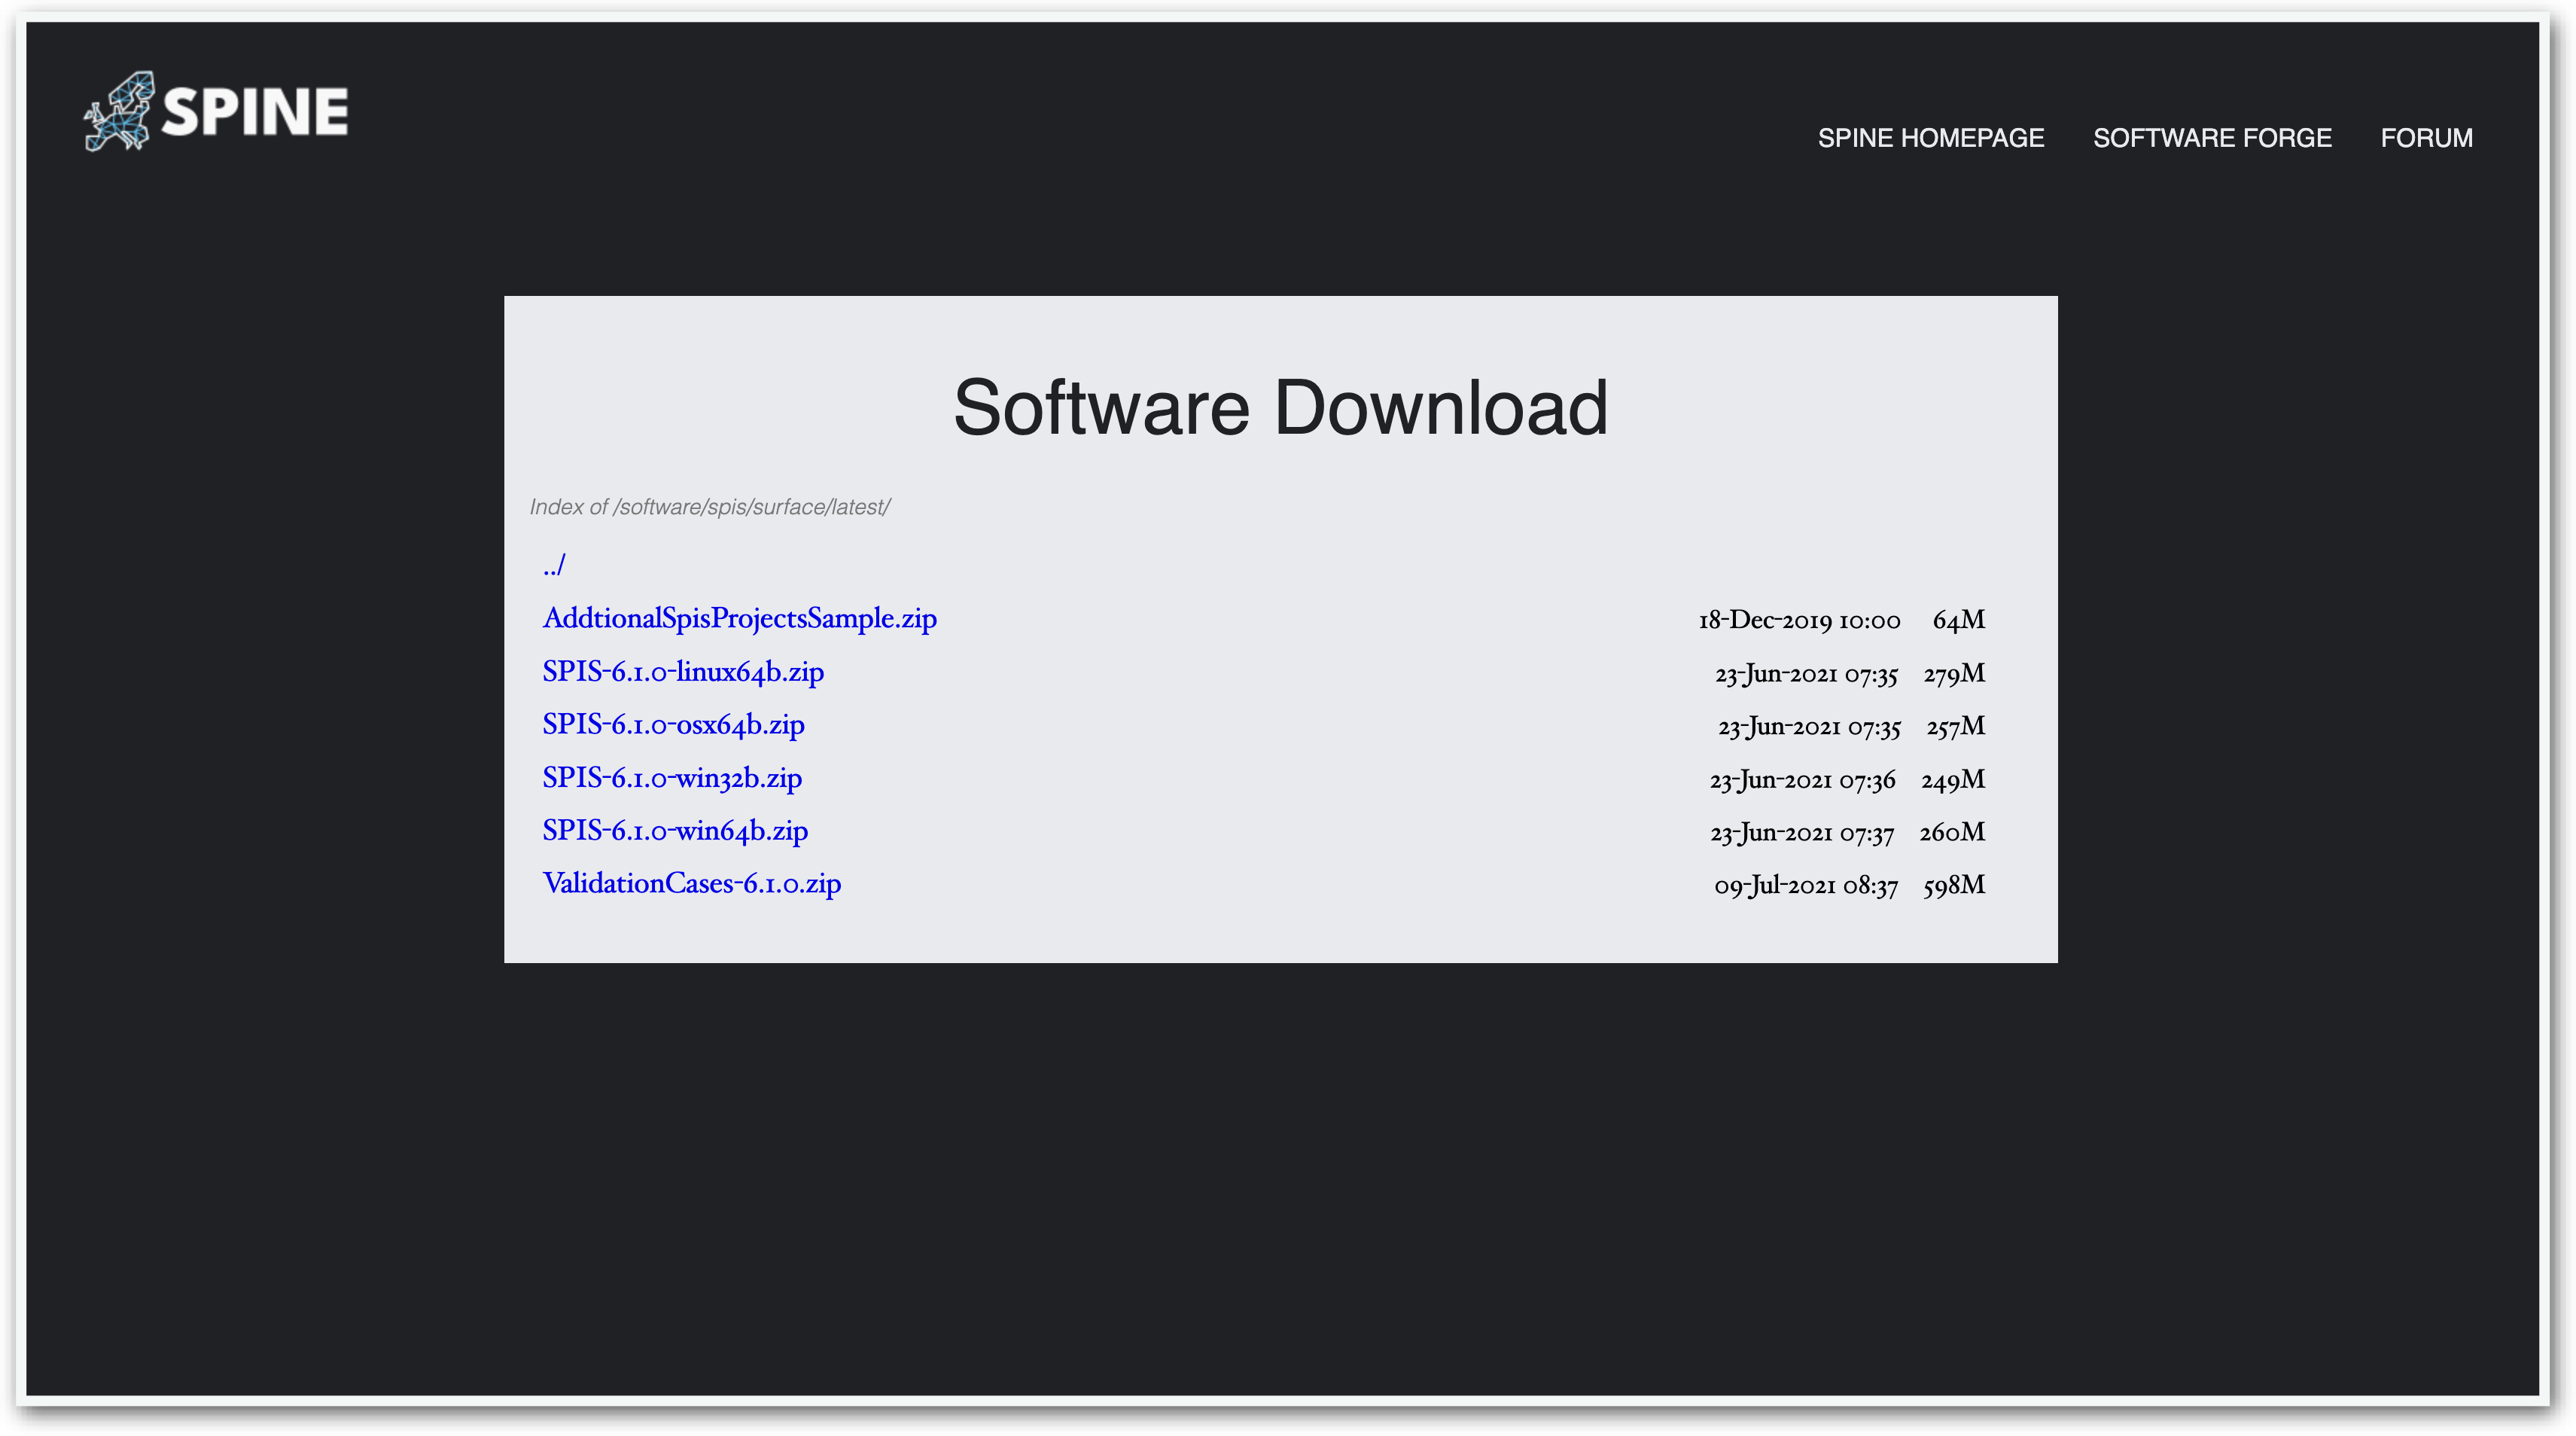
\includegraphics[width=0.45\textwidth]{fig1.jpg}
    \caption{The page where SPIS can be downloaded.}
\end{figure}

\begin{figure}[!ht]
    \centering
    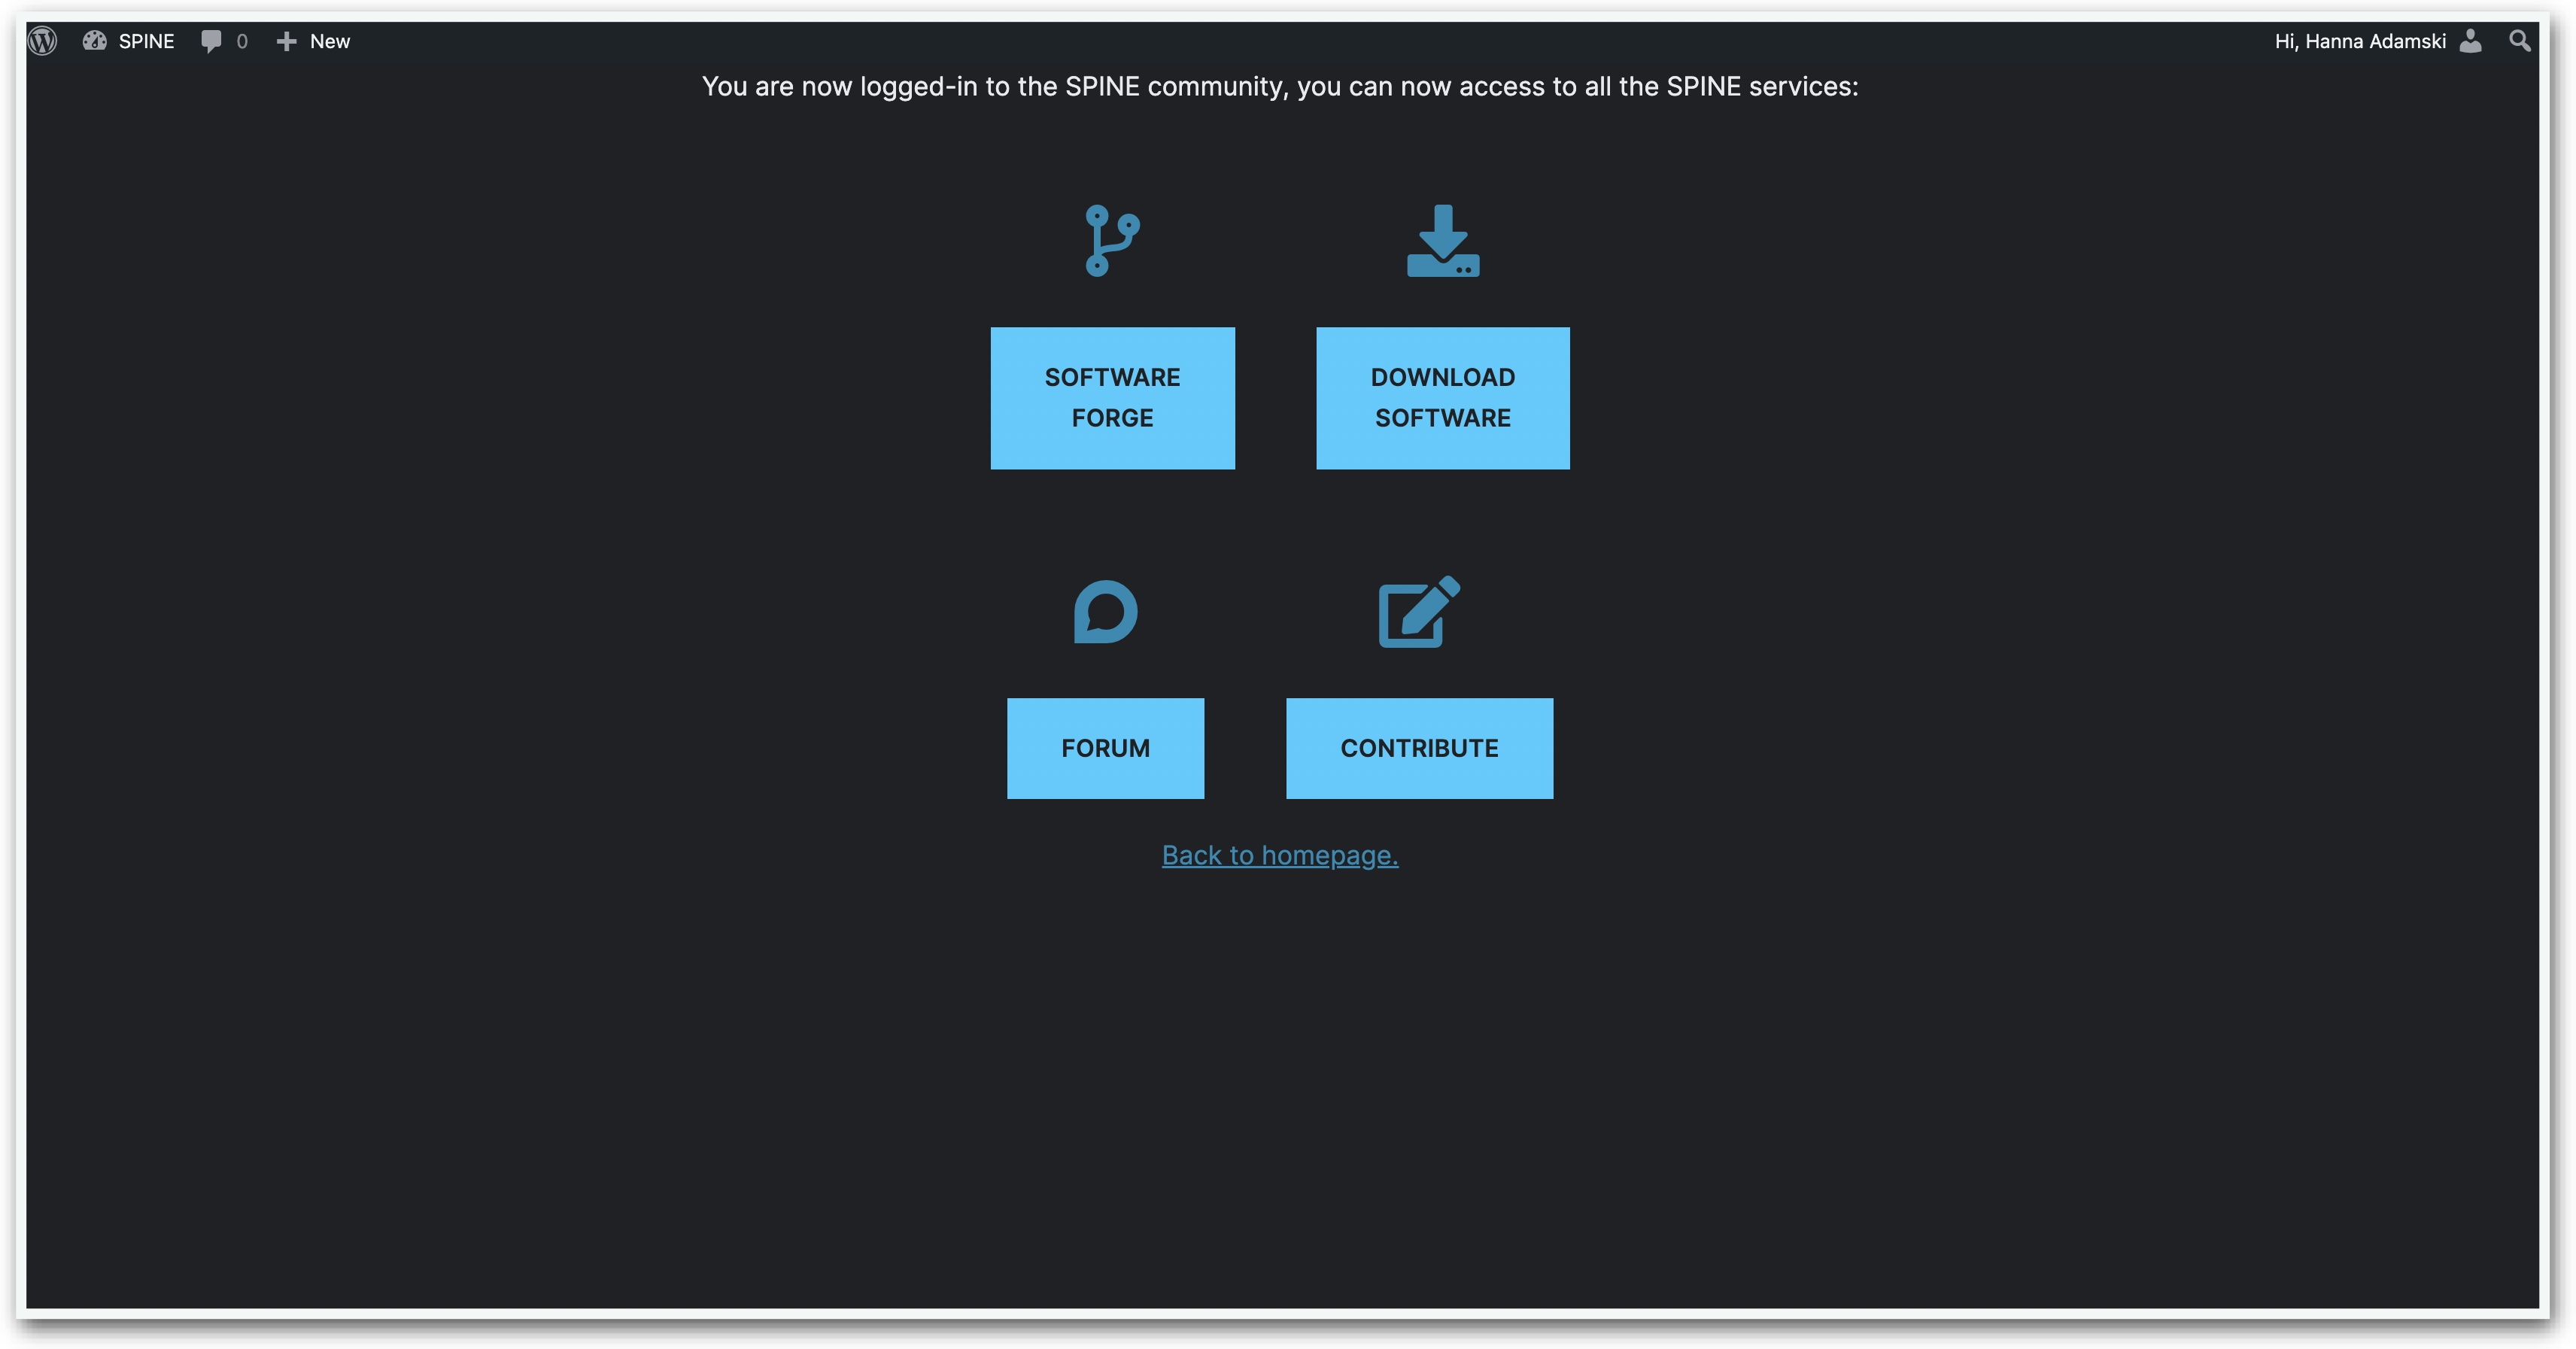
\includegraphics[width=0.45\textwidth]{fig2.jpg}
    \caption{The webpage where SPIS can be downloaded, following authentication via a registered user account.}
\end{figure}

\begin{figure}[!ht]
    \centering
    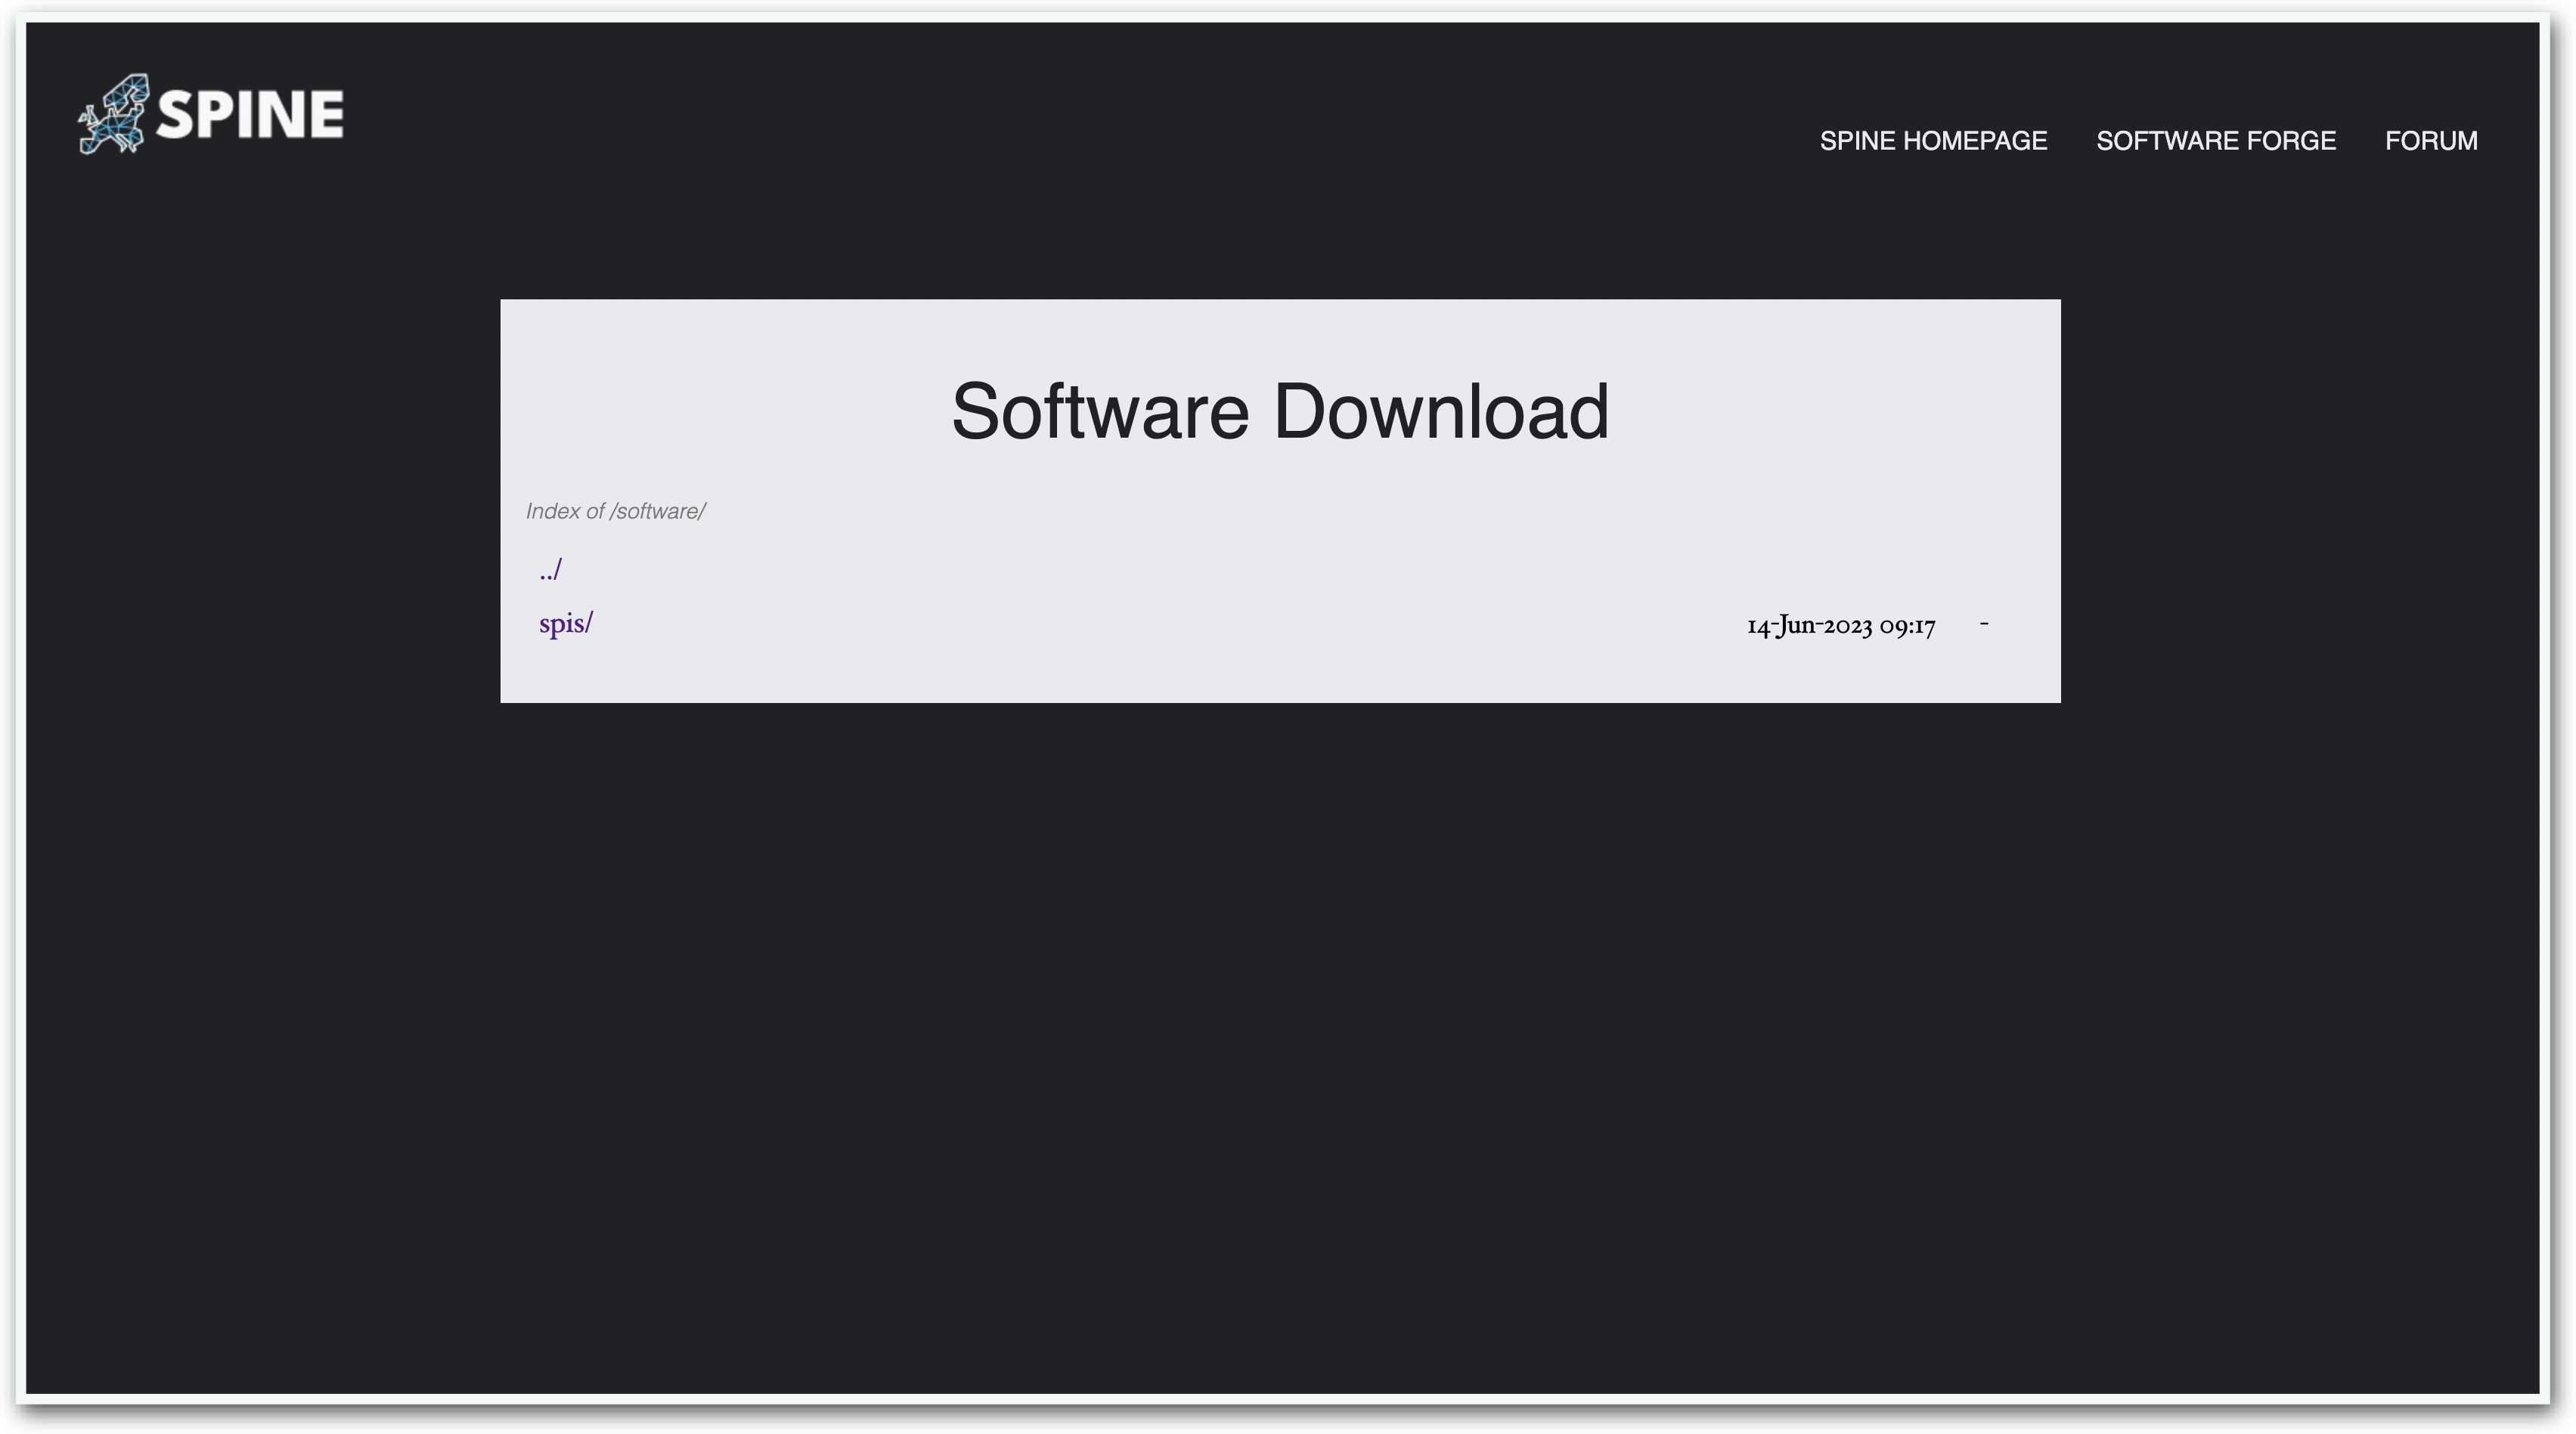
\includegraphics[width=0.45\textwidth]{fig3.jpg}
    \caption{The page that appears after selecting "Download software".}
\end{figure}

The minimum hardware requirements to properly run SPIS are typically met by any computer manufactured after 2005. However, if SPIS is installed on an external server \textbf{make sure that the server has a graphic card with more than 128 Mb of video memory.} If this is missing from the server, the graphical user interface of SPIS cannot be launched, making it impossible to visually track the simulation steps. This will significantly hinder the simulation process, in particular when starting new projects.\par
After downloading and extracting SPIS, move the "SPIS-6.1.0" folder from the Download folder to the preferred application folder.\par
To use SPIS, a mesh generator called Gmsh is required. Although Gmsh is a separate software, it is included in the SPIS download package. However, the version of Gmsh included may not be compatible with certain systems, particularly those using a Mac with an M-series chip. In such cases, the macOS (ARM) version of Gmsh should be downloaded directly from the Gmsh website: \url{https://gmsh.info}.

\subsection{Simulation set-up}

In order to run SPIS simulations, the following steps are required:
\begin{enumerate}
    \item Build a spacecraft geometry, covered by chapter 1.4
    \item Generate a computational mesh, covered by chapter 1.5
    \item Define the material library of the spacecraft, covered by chapter 1.7
    \item Define the circuitry of the spacecraft, covered by chapter 1.8
    \item Define the spacecraft environment, covered by chapter 1.9
\end{enumerate}
All these steps will be covered in order, using a simplified spacecraft geometry, a basic cube, to simulate the surface charging of a spacecraft in the ionosphere of Jupiter's moon Ganymede at an altitude of 400 km, as an example.

\subsection{Building the spacecraft 3D model}

All these steps will be covered in order, using a simplified spacecraft geometry, a basic cube, to simulate the surface charging of a spacecraft in the ionosphere of Jupiter's moon Ganymede at an altitude of 400 km, as an example.
\begin{enumerate}[label=\Alph*.]
    \item The model can be built in SPIS using the "Edit geometry file" option.
    \item The Gmsh user interface can be used to build the geometry file.
    \item For very simple geometries, the easiest option is often to create a txt file and load it into Gmsh.
\end{enumerate}
For our example we will use option C.\par
A common problem when running SPIS simulations is that the simulation mesh is not properly defined. It is therefore not recommended to build a complex spacecraft model before moving on to step 2 to 5 of setting up the simulation. Start instead with a very simple spacecraft model, preferably just a square or cylinder with the relevant proportions and run a first simulation using that geometry. This approach helps ensure that the rest of the simulation inputs are in order, before investing time in developing a more detailed spacecraft model. It supports the creation of a robust  simulation set up by isolating potential issues related to the simulation mesh from those associated with the other input parameters, defined in step 3 to 5 of the simulation set up process.\par
When building a geometry in Gmsh start by defining the coordinates of the points that is the foundation of the spacecraft geometry. An example is shown in Figure 4.\par
We will begin with building a simple cube that represents the spacecraft, as shown in Figure 4. The parameters (l and b) that are defined in the beginning of the file gives the resolution of the mesh at the surface of the spacecraft, here called l, and at the outer boundary of the mesh, here called b.\par
The Points give the coordinates for the points that define the geometry and also the mesh resolution at that specific point. For example, Point(100) = {-1, -1, -1, l}; states that a point with ID number 100 should be located at x = -1, y = -1, z = -1 and the mesh connected to this point should have mesh resolution l, which is given a length of 0.1 m in the lines above. Points 100 to 107 gives the corner points of the sphere. We also have to define the outer boundary of our computational volume, these are given by Points 108 to 114. Please be careful to use a large enough simulation geometry around the spacecraft, if the simulation volume is too small this will provide erroneous results. Large enough means that the computational volume should include any changes to the local environment caused by the presence of the spacecraft, this size will depend on the environment and spacecraft design. In this example we start with a volume with a diameter of 60 m for a cube shaped spacecraft with sides of 2 m.

\begin{figure}[!ht]
    \centering
    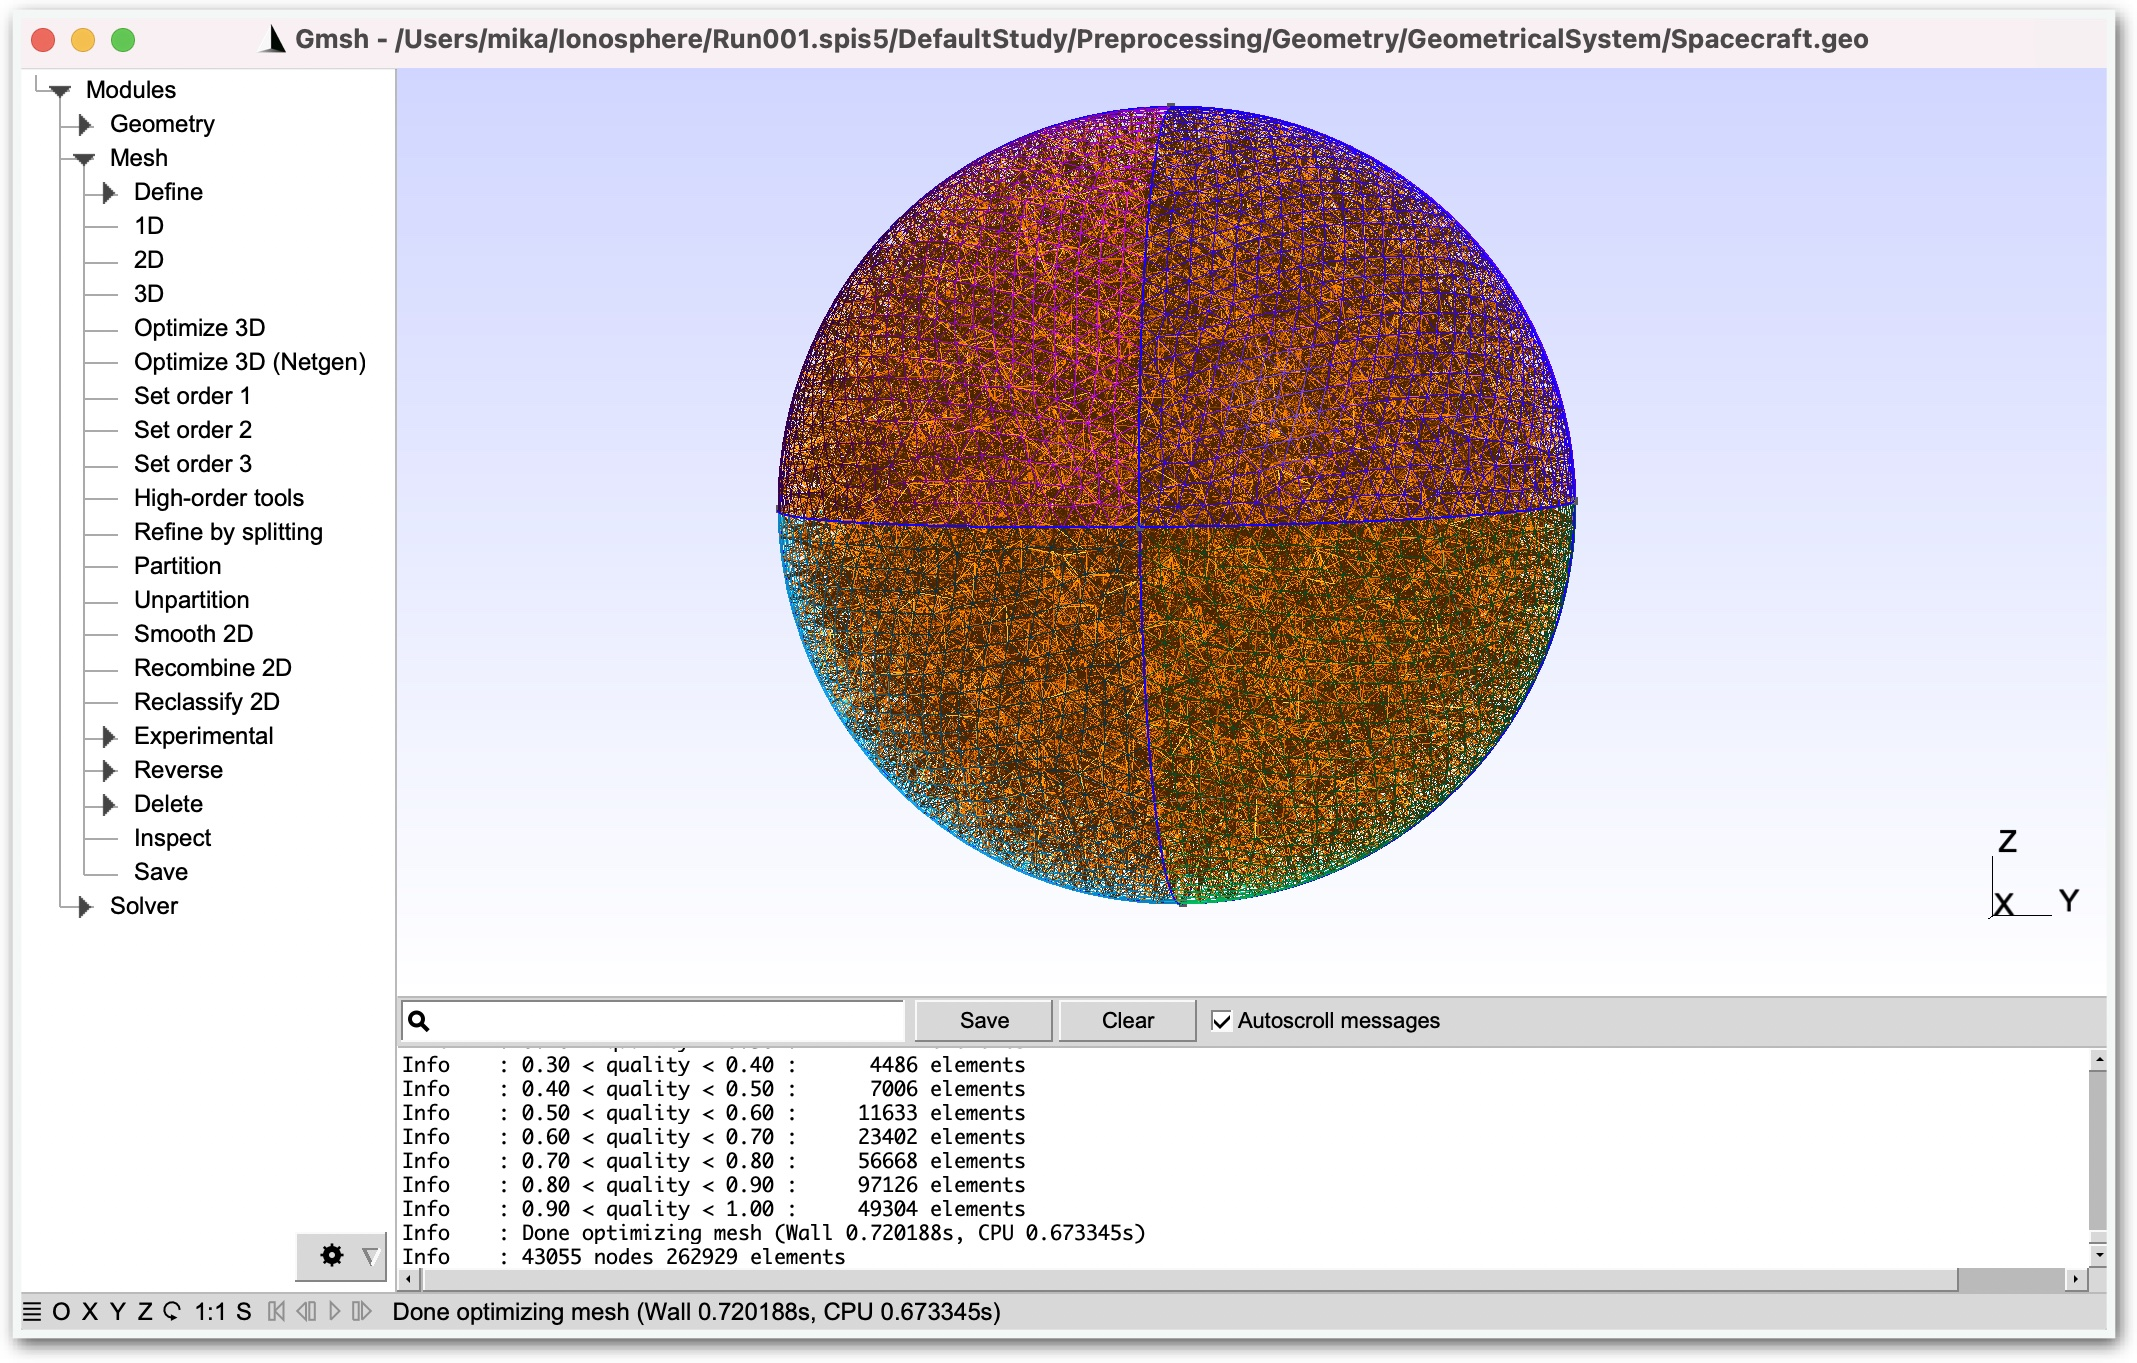
\includegraphics[width=0.45\textwidth]{fig4.jpg}
    \caption{The beginning of the file that defines the spacecraft geometry.}
\end{figure}

After defining the points, define lines that connect the points, as shown in Figure 5. Here the three most commonly used options are
\begin{enumerate}
    \item Line, which is only used for straight lines
    \item Circle, which is only used for sections of circles
    \item Ellipse, which is used for sections of ellipses
\end{enumerate}
For example, Line(200) = {100, 101}; states that a line with ID number 200 should be located between the points with ID numbers 100 and 101. The direction of the line does not matter in this instance, so Line(200) = {100, 101}; and Line(200) = {101, 100}; will give the same result.\par
In Gmsh, the circle sections must be smaller than 180 degrees to ensure that the software correctly identifies the corresponding arc. The first point defines the start of the arc, the second defines the center of the circle and the third defines the end of the arc. After defining the lines, each surface must be defined, as shown in Figure 6. It is important to distinguish between surfaces with different materials, since the second step of the simulation set up is to define the materials and their properties. At that stage, each surface material must be defined individually. To define a surface, begin by listing the lines that form the boundary of that surface. For instance, Line Loop(300) = {200, 201, 202, 203}; states that the lines with ID numbers 200, 201, 202, and 203 form a closed line loop with ID number 300. This closed line loop defines a plane surface so use Plane Surface (301) = {300}; to state that the surface with ID 301 is the surface within the Line Loop with ID 300.

\begin{figure}[!ht]
    \centering
    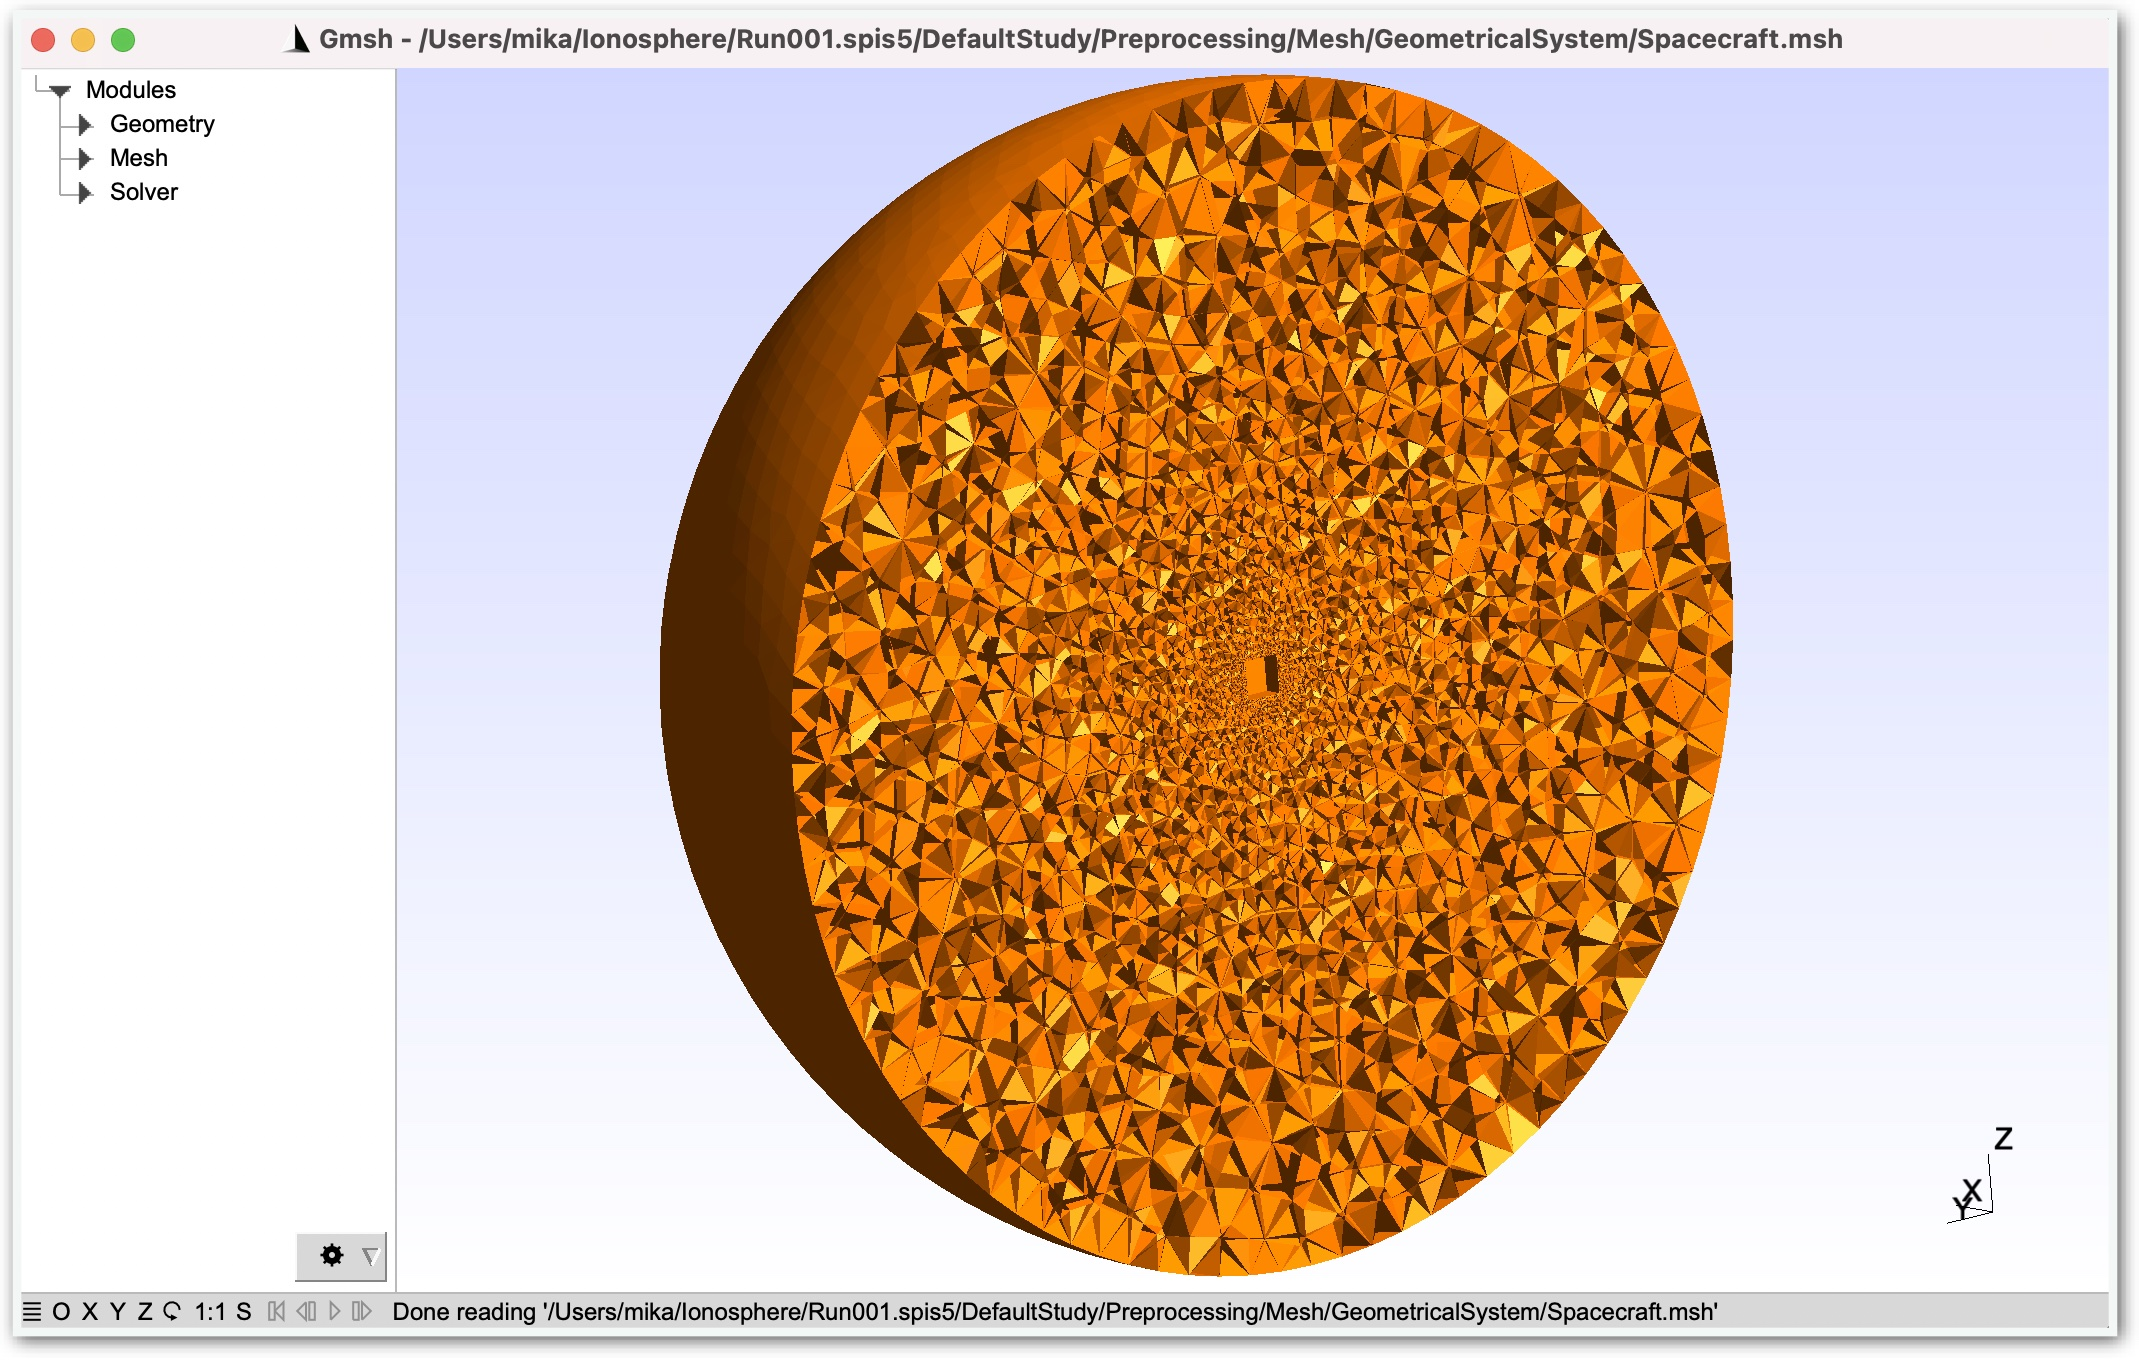
\includegraphics[width=0.45\textwidth]{fig5.jpg}
    \caption{The lines that connects the points of the spacecraft geometry.}
\end{figure}

\begin{figure}[!ht]
    \centering
    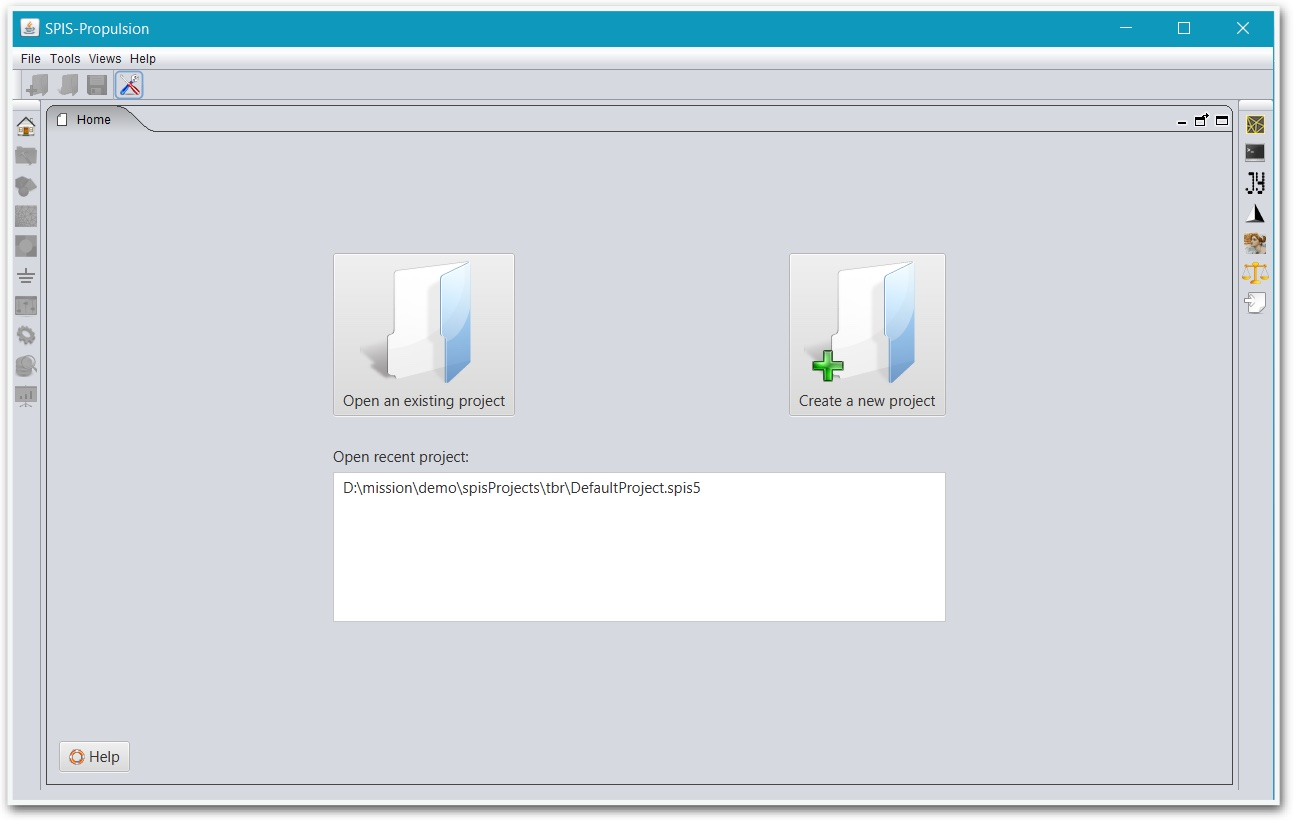
\includegraphics[width=0.45\textwidth]{fig6.jpg}
    \caption{How to define the surfaces of the spacecraft model.}
\end{figure}

The directions of the enclosed lines that make up a surface are crucial. For example, Line Loop 312 is made up of the line segments 212, 221 and 216, but the directions of the lines are not all the same. Line 212 is defined from Point 109 to 110, Line 221 is defined from Point 113 to 110, and Line 216 is defined from Point 109 to 113. Hence, by reversing the direction of lines 221 and 216 a closed loop is formed with all segments oriented in the same direction. The order of the points will then be 109, 110, 113 and back to 109. Alternatively, the line loop can be defined in the opposite direction as {-212, 221, 216}, which would achieve the same result. Since it is easy to make mistakes at this step, it is imperative to double check wether the line loops are correctly defined before moving on. This can be done by opening the geometry file in Gmsh. Click on the Gmsh icon in the Application folder and choose "File" and "Open" and choose the geometry file. For the simple geometry that we are using here, this opens a window like the one in Figure 7. If the Gmsh version included in the downloaded SPIS package is being used, Gmsh can be found within the SPIS folder in "dependencies/thirdparty".\par
The blue circle shown in Figure 7 is the outer boundary of the computational volume and the small square represents the spacecraft. If one of the line loops has been defined incorrectly, the window would look like in Figure 8. Please note the red error message displayed at the bottom of the window.

\begin{figure}[!ht]
    \centering
    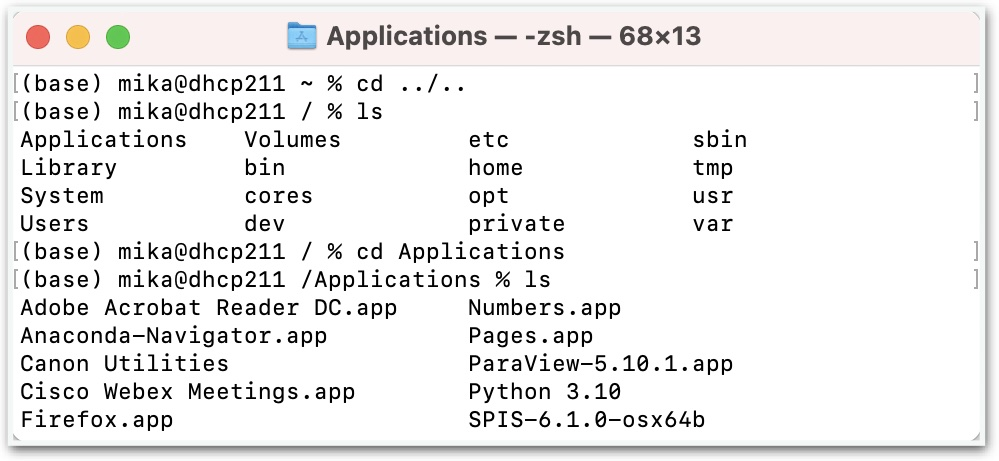
\includegraphics[width=0.45\textwidth]{fig7.jpg}
    \caption{The spacecraft geo file opened in Gmsh.}
\end{figure}

\begin{figure}[!ht]
    \centering
    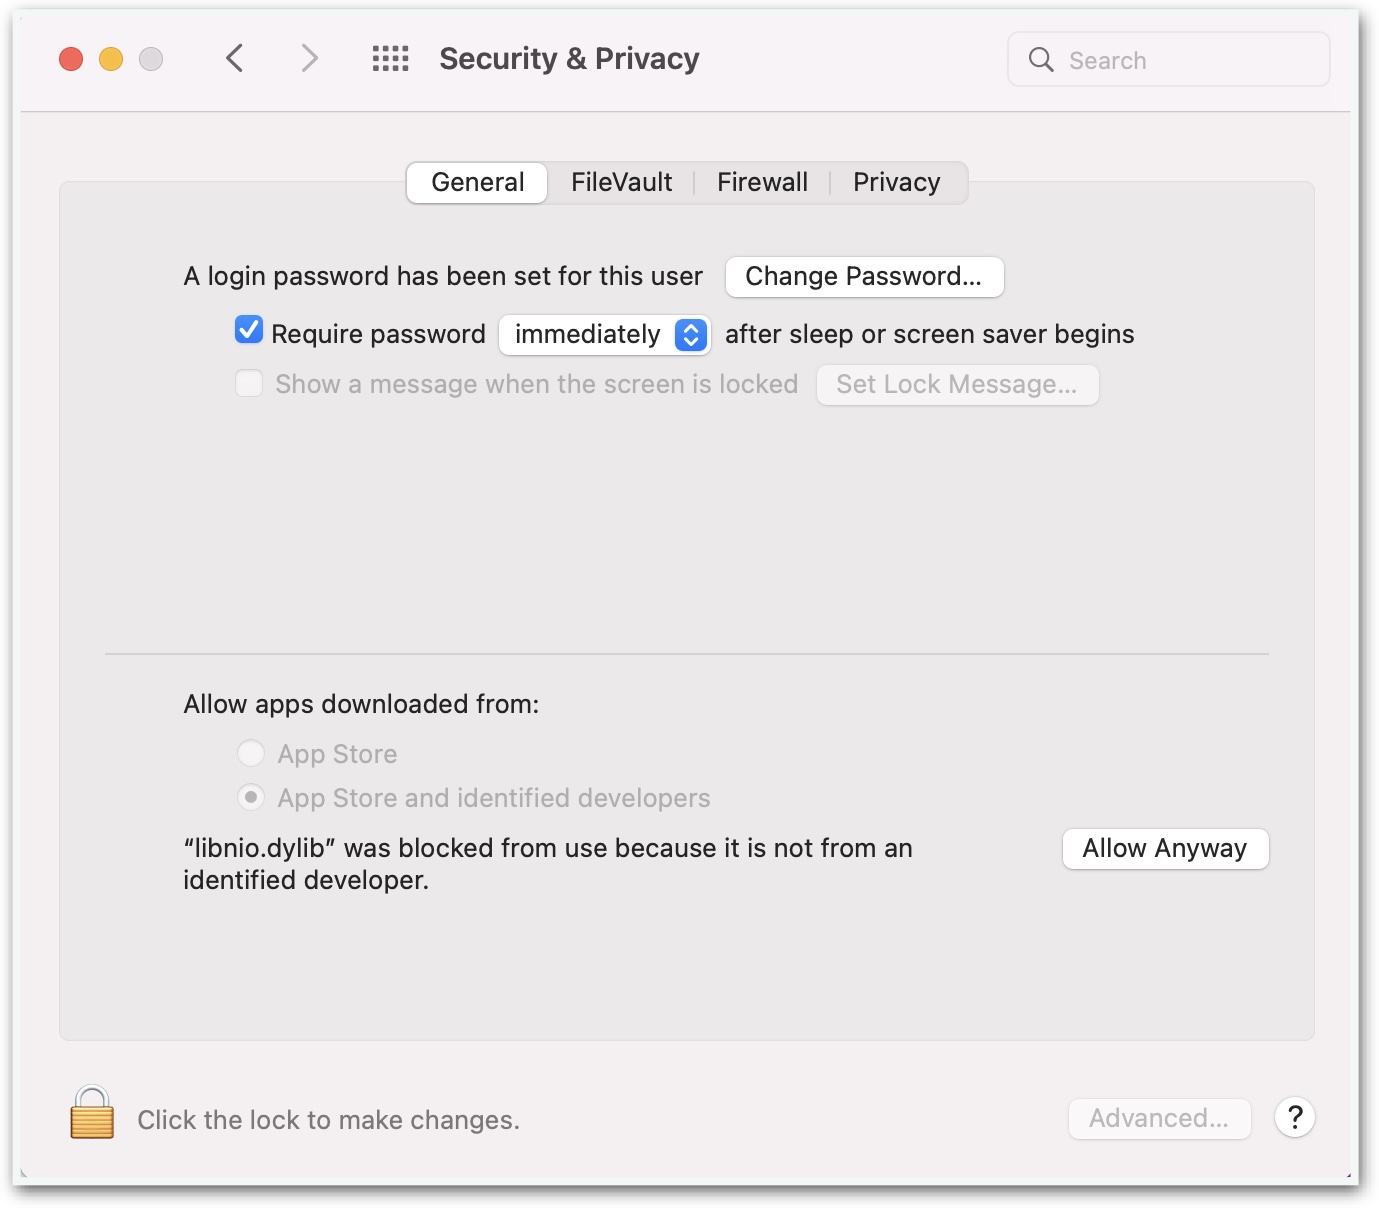
\includegraphics[width=0.45\textwidth]{fig8.jpg}
    \caption{The red text shows the error message of Gmsh.}
\end{figure}

The error message shows that something is defined incorrectly. Clicking on the red line reveals the full error message: Curve loop 312 is wrong, Wrong definition of surface 313: 1 borders instead of 3 or 4. Rotating the geometry and zooming in allows for visual inspection to ensure that all the points and lines are properly defined, as can be seen in Figure 9.\par
To verify that all the surfaces are correctly defined press "Tools", "Options", "Geometry" and mark "Surfaces". This will include grey dashed lines crossing all the defined surfaces, as shown in Figure 10. Enabling the "Volumes" option reveals a yellow sphere at the center of the computational volume. Defining the computational volume begins with creating a Surface Loop, as shown in Figure 11. For example, Surface Loop(400) = {301, 303, 305, 307, 309, 311}; states that a surfaces loop with ID number 400 contains all the plane surfaces of the sphere that represents the spacecraft. Surface Loop 401 contains all the surfaces of the outer boundary. To define the computational volume use Volume(500) = {401, 400}; where the inner surface loop 400 is subtracted from the outer surface loop 401, resulting in a volume between the spacecraft model and the outer boundary, which is the computational volume. It is important to make sure that all volumes are closed volumes and that no surfaces are missing.

\begin{figure}[!ht]
    \centering
    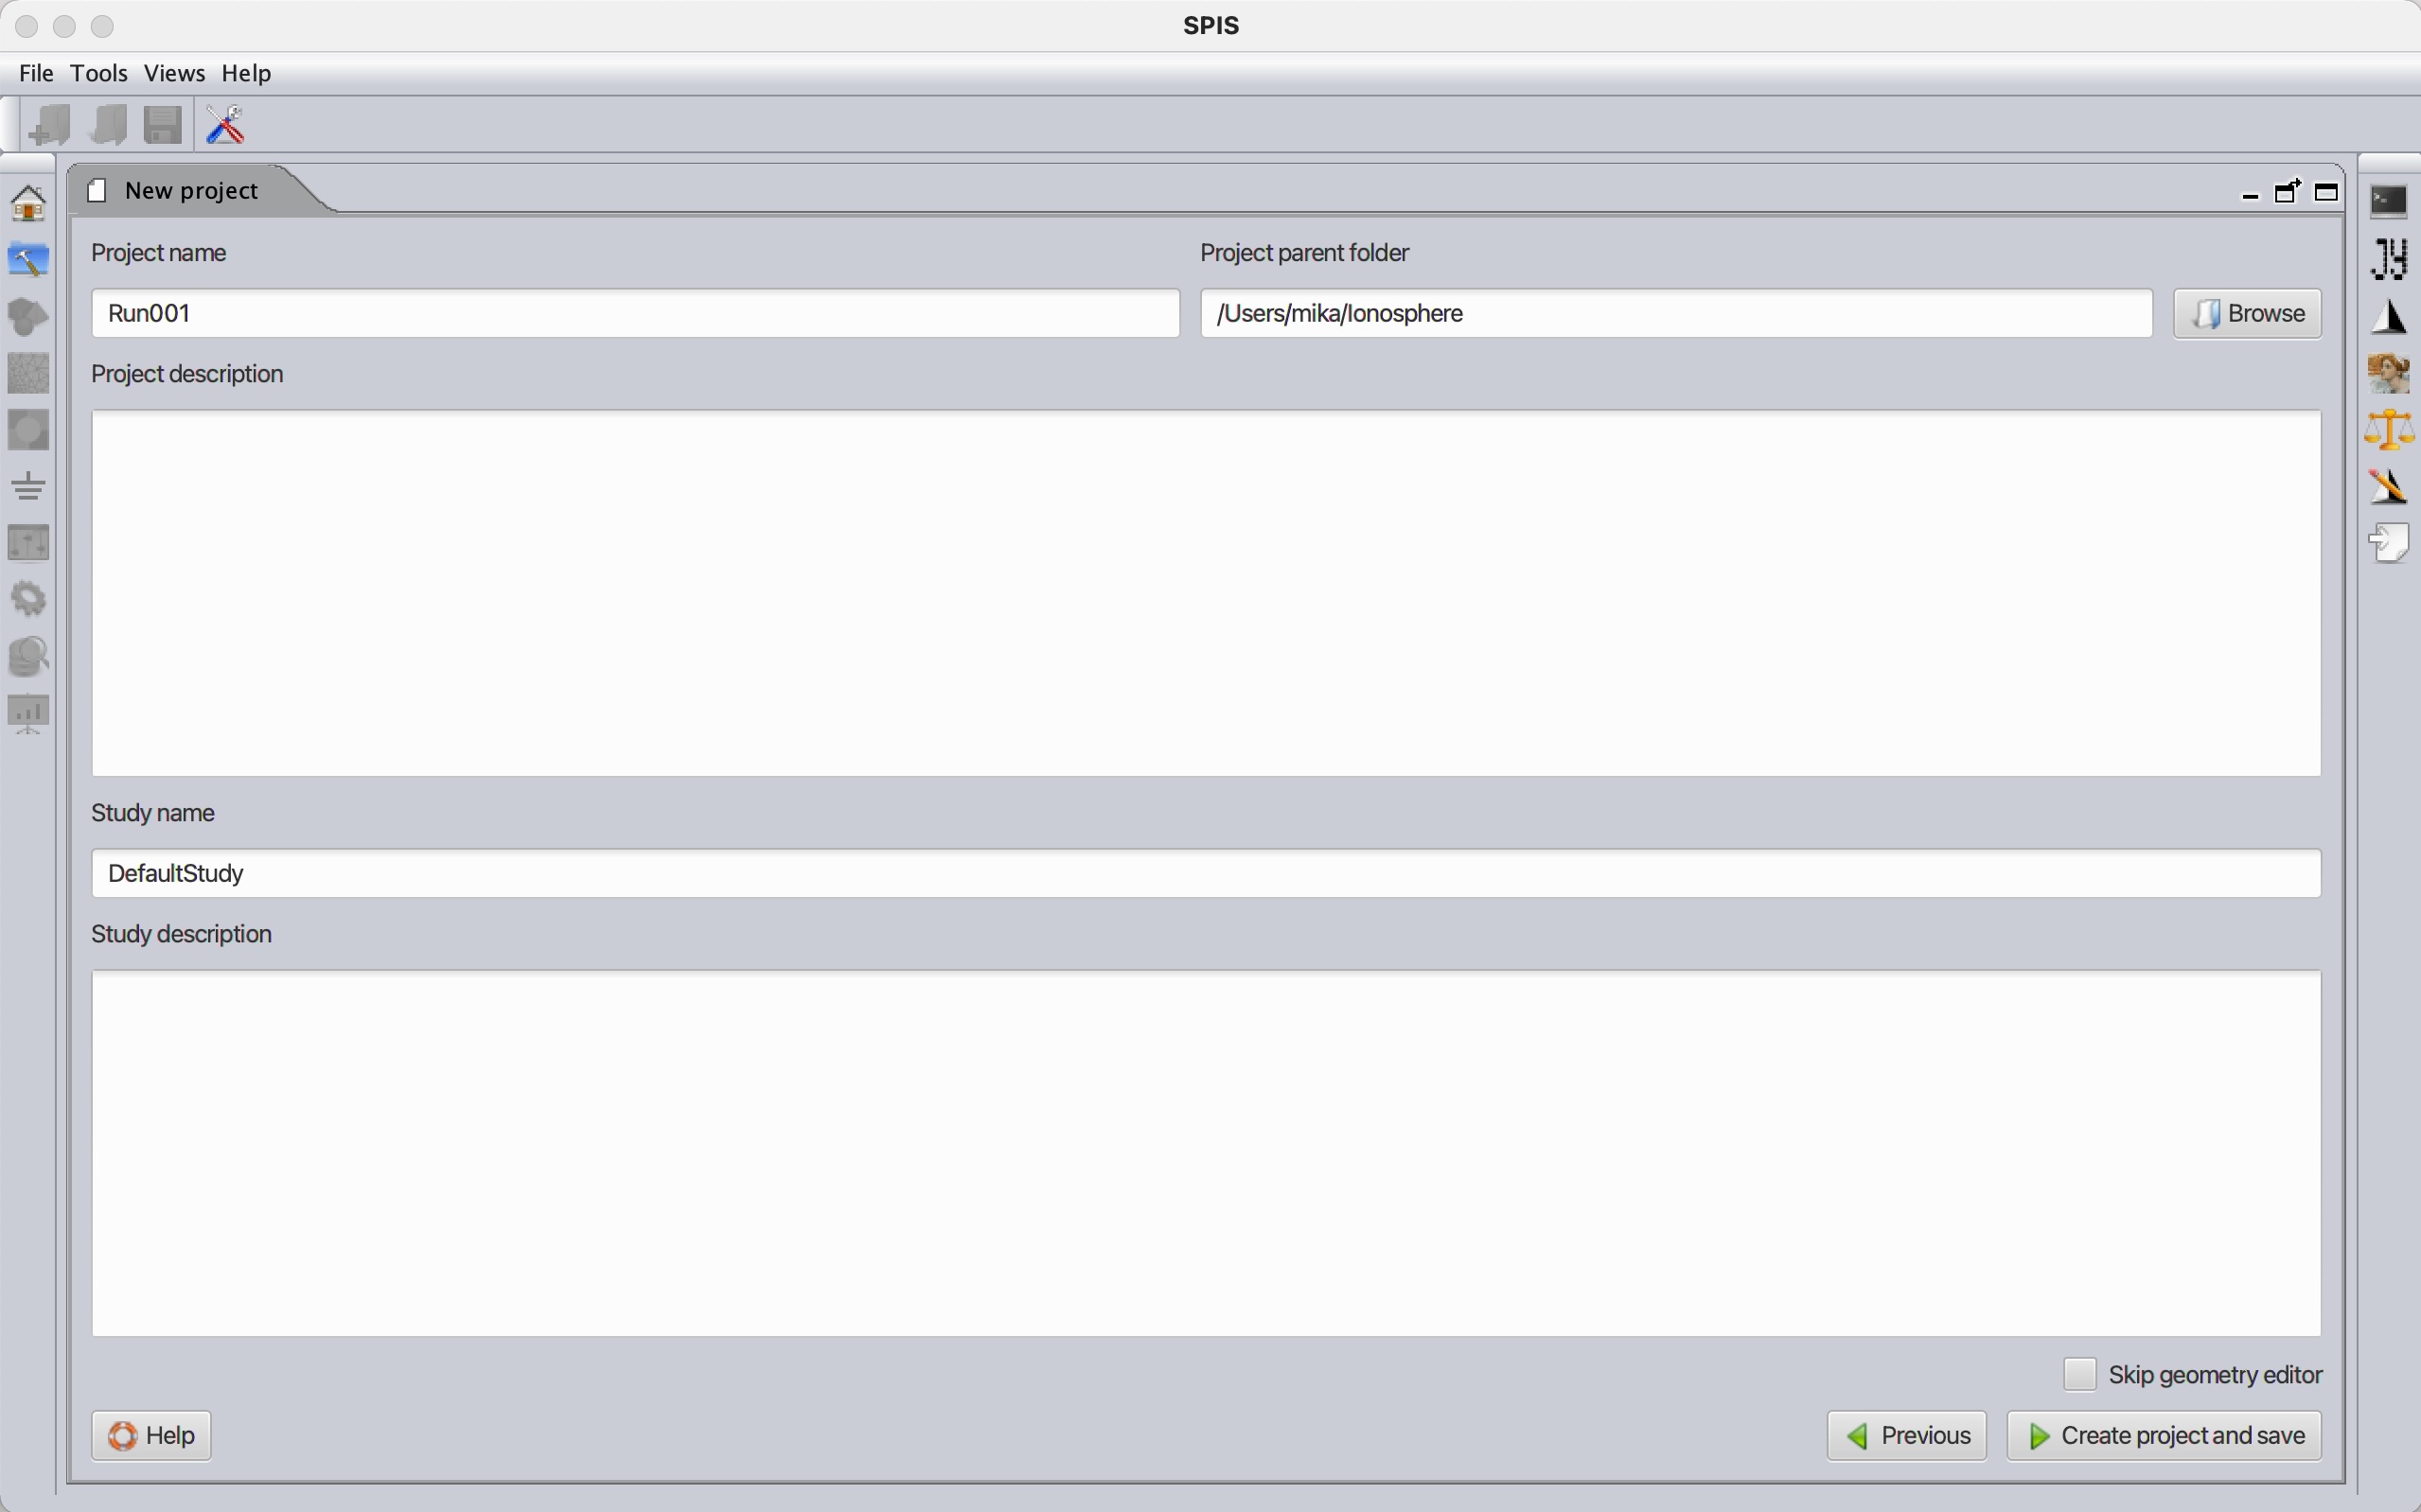
\includegraphics[width=0.45\textwidth]{fig9.jpg}
    \caption{The geometry can be rotated and enlarged.}
\end{figure}

\begin{figure}[!ht]
    \centering
    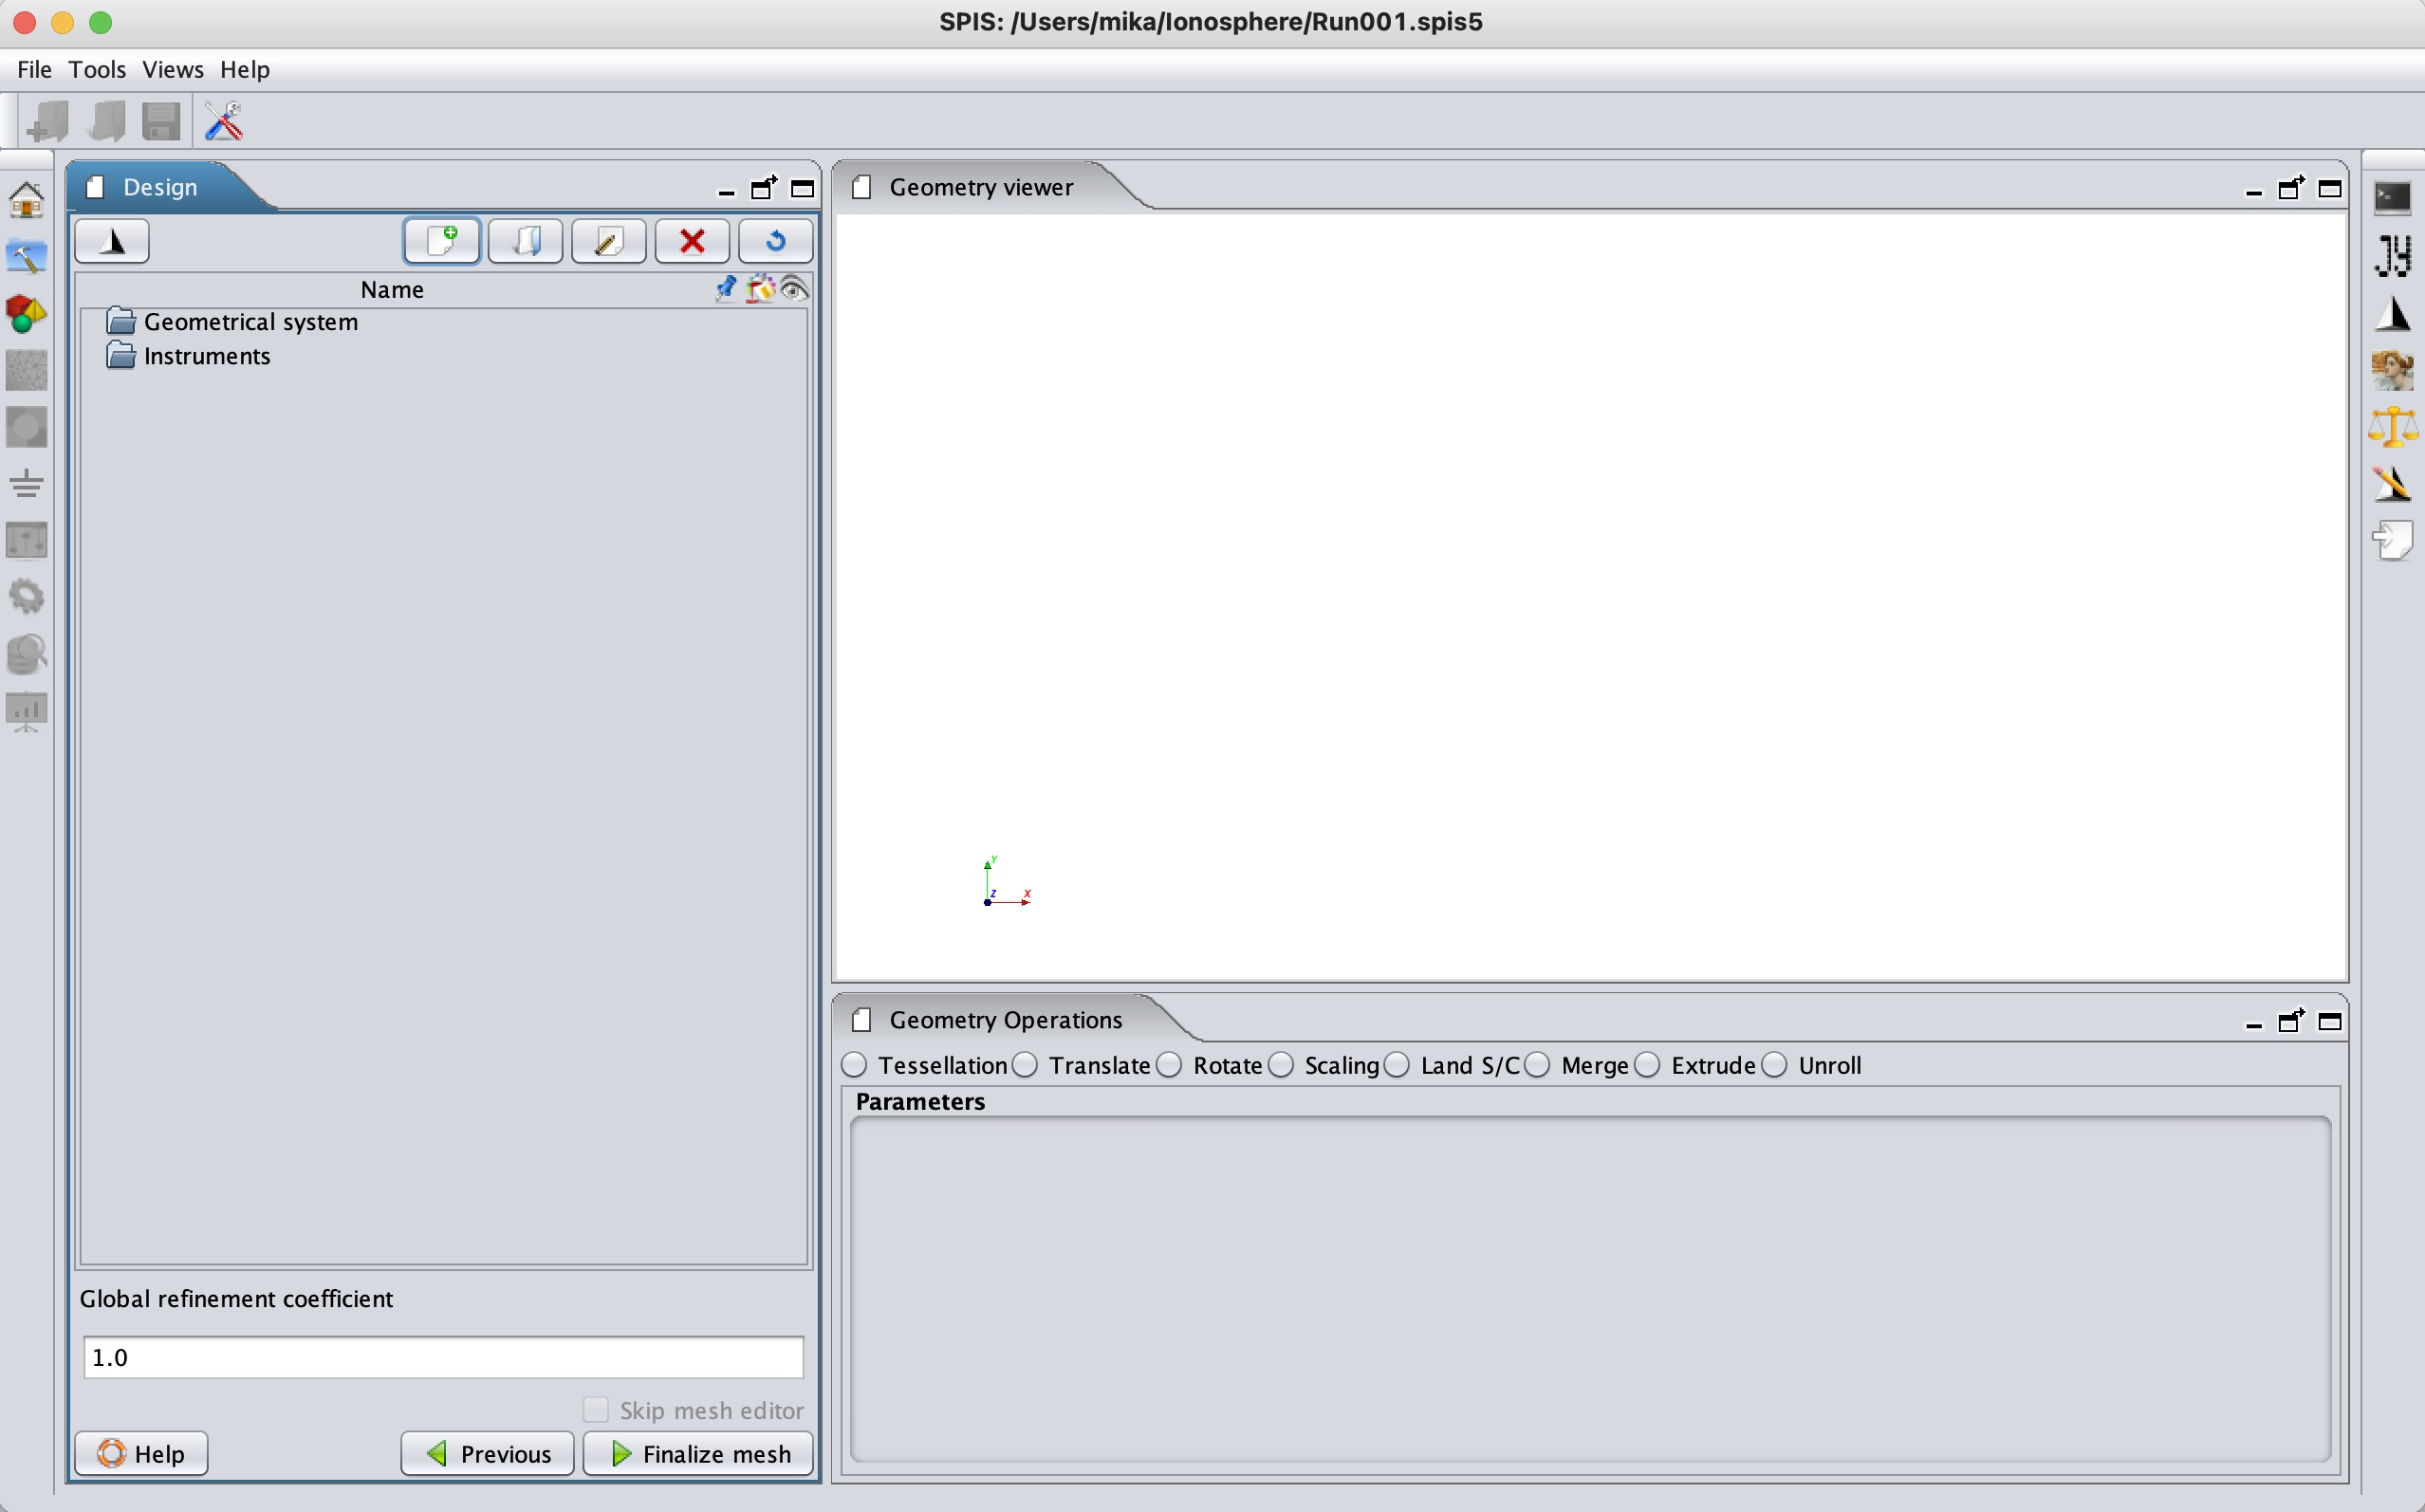
\includegraphics[width=0.45\textwidth]{fig10.jpg}
    \caption{The surfaces are crossed by grey dashed lines.}
\end{figure}

After defining all the points, lines, surfaces and volumes, these entities have to be grouped together into what in Gmsh is called physical surfaces and volumes. An example is shown in Figure 11. The Physical Volume should be the same computational volume as defined earlier.

\begin{figure}[!ht]
    \centering
    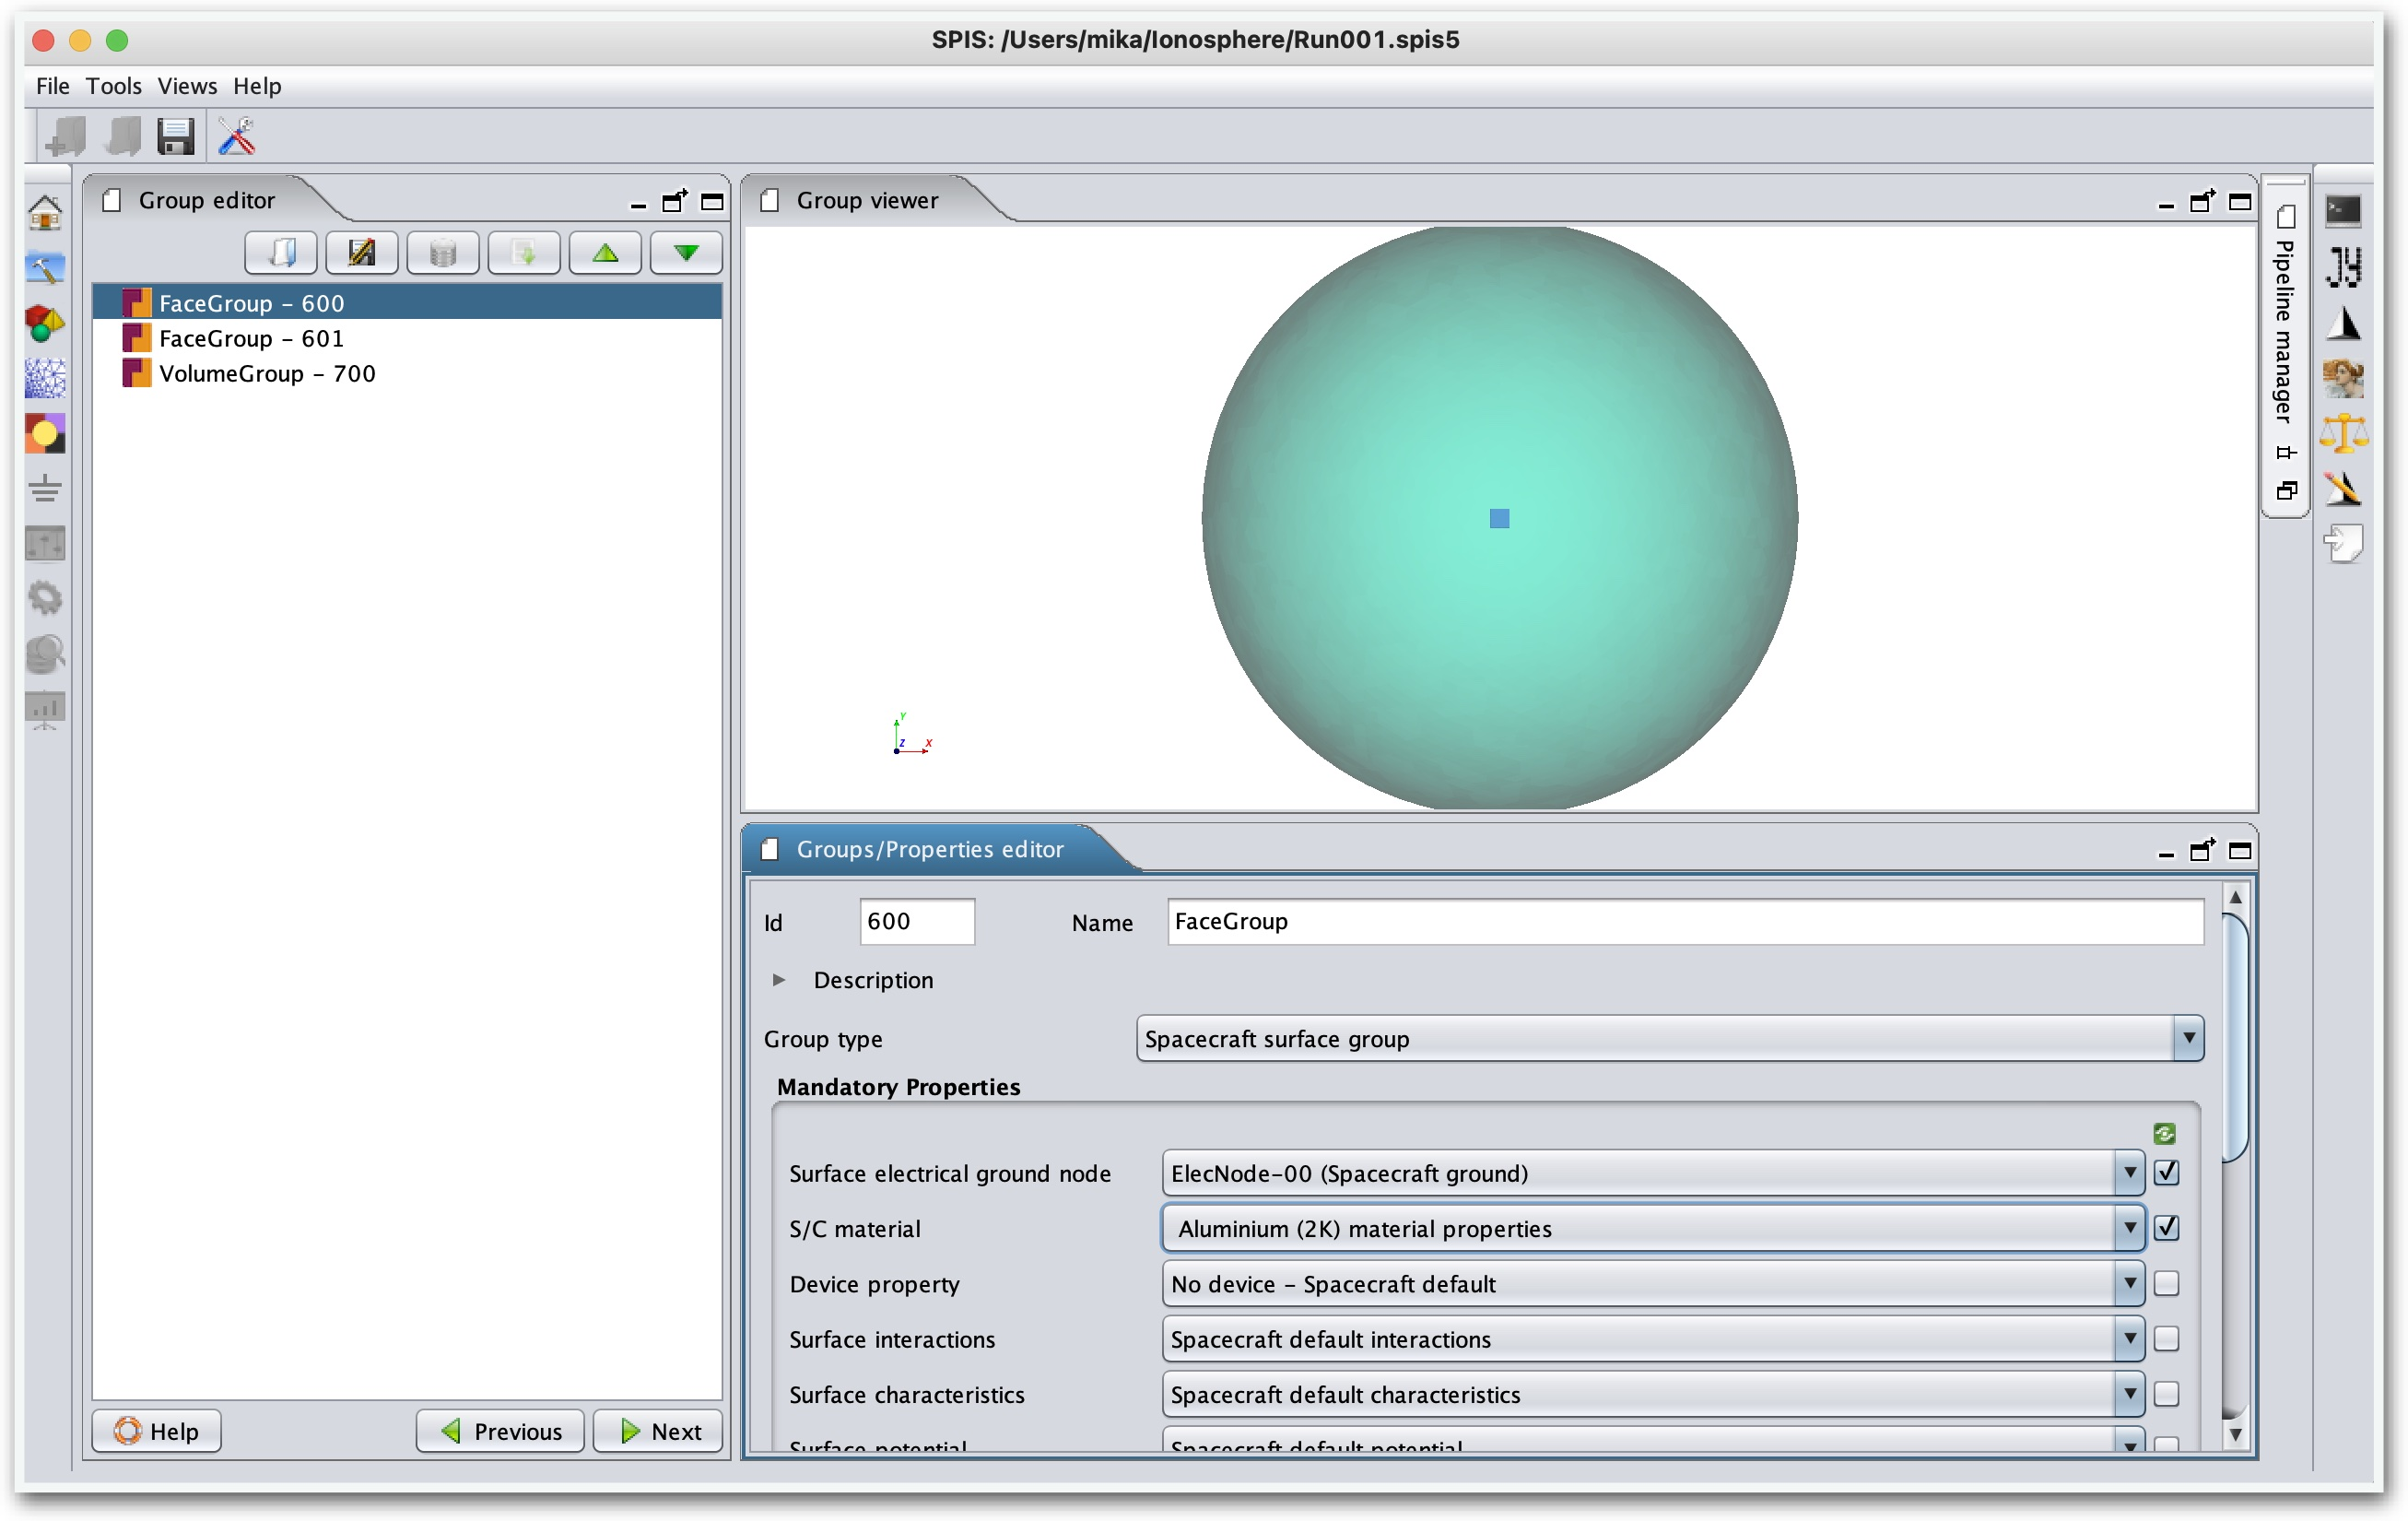
\includegraphics[width=0.45\textwidth]{fig11.jpg}
    \caption{Example of how to define the volumes and physical groups.}
\end{figure}

\subsection{The computational mesh}

The next step is to build the mesh of the computational volume. This can be done in both Gmsh and SPIS. In Gmsh, use the menu on the left hand side of the window, choose "Mesh" and then "3D". The mesh should then be visible in the computational volume, as shown in Figure 12.\par
Mesh generation includes an optimisation process that removes low-quality elements which could otherwise lead to computational issues. There are also methods to optimise the mesh even further, such as the "Optimize 3D" or "Optimize 3D (Netgen)", these methods also reduce the number of mesh elements. Based on experience, the best outcome is usually from using the "Optimize 3D (Netgen)". Mesh improvements can be monitored using the "Tools" and "Statistics" window. For example, when creating the mesh shown in Figure 12, the initial mesh contains 249,626 tetrahedral elements. After applying the "Optimize 3D (Netgen)" once, this number is reduced to 216,805.

\begin{figure}[!ht]
    \centering
    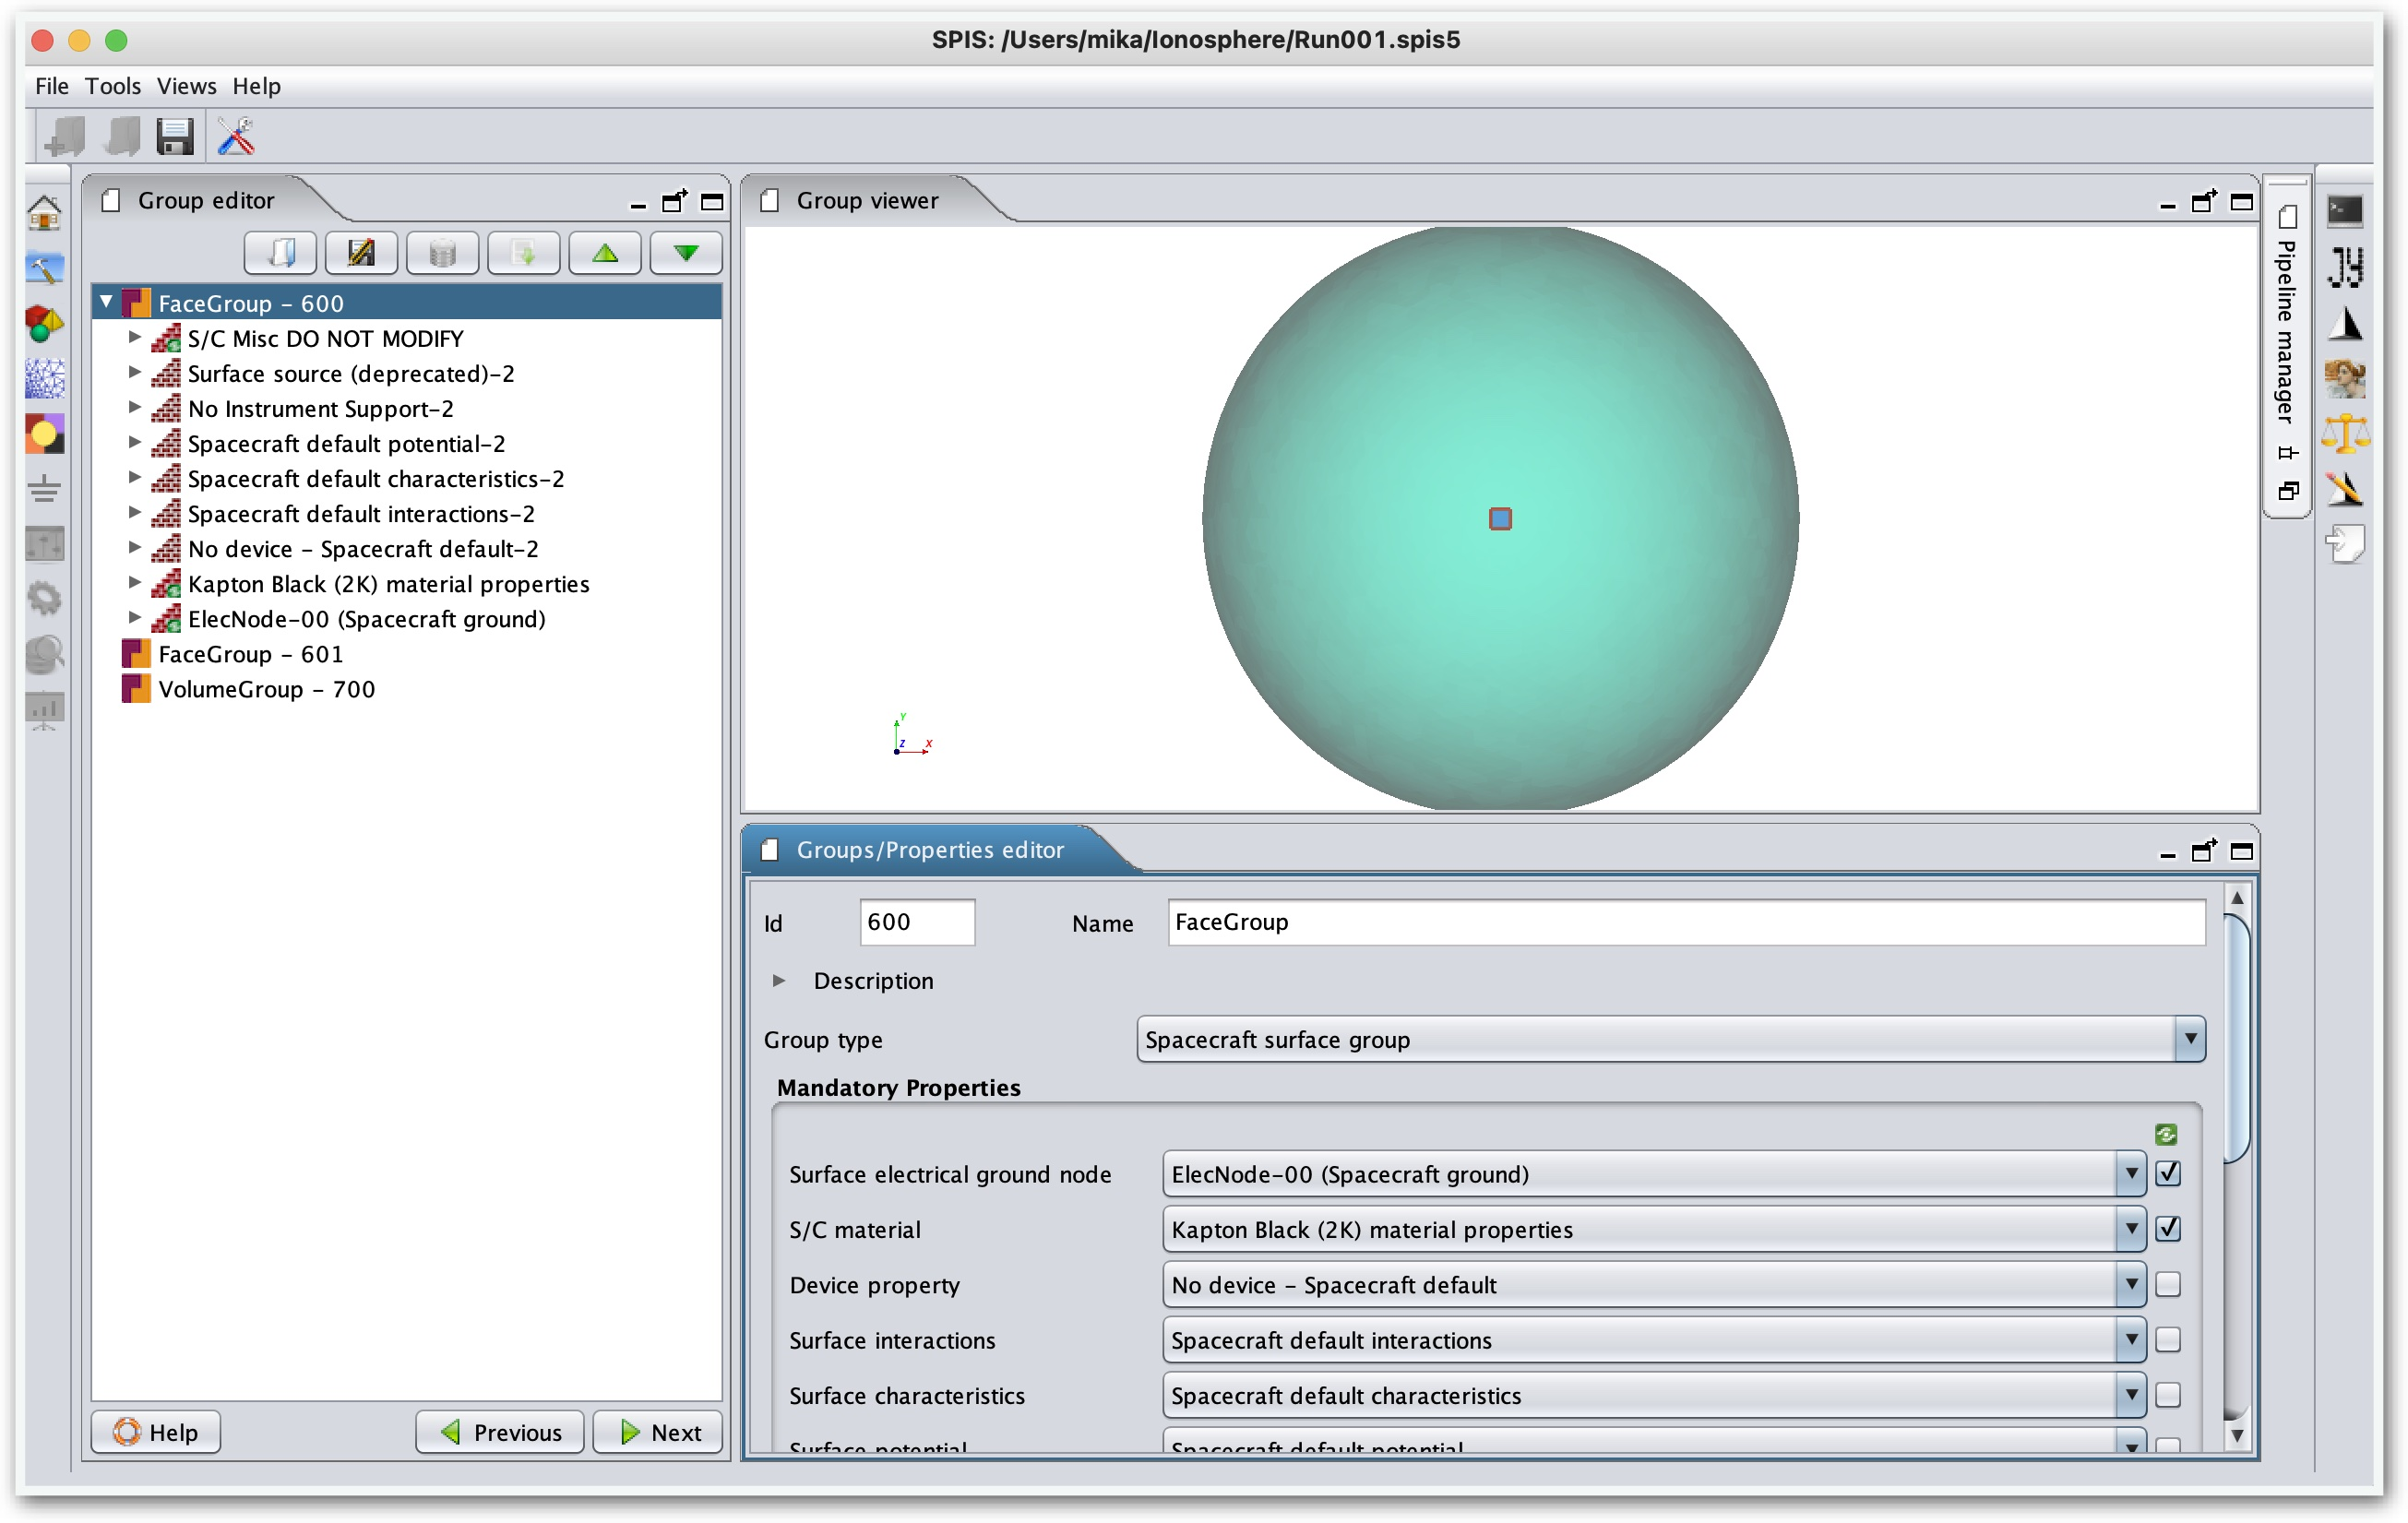
\includegraphics[width=0.45\textwidth]{fig12.jpg}
    \caption{The mesh of the computational volume.}
\end{figure}

A useful way to check that the volumes and the mesh is defined correctly is to look at the image of the 3D element faces, as shown in Figure 13. Open "Tools" and "Options", choose "Mesh" and remove the markers from "2D element edges" and "3D element edges" and make "3D element faces" visible. Then open "Tools" and "Clipping", choose "Mesh".  If using 1 for parameter A in Plane 0, the computational mesh will be cut in half, as shown in Figure 13. Move the object to see the cross-section of the mesh.

\begin{figure}[!ht]
    \centering
    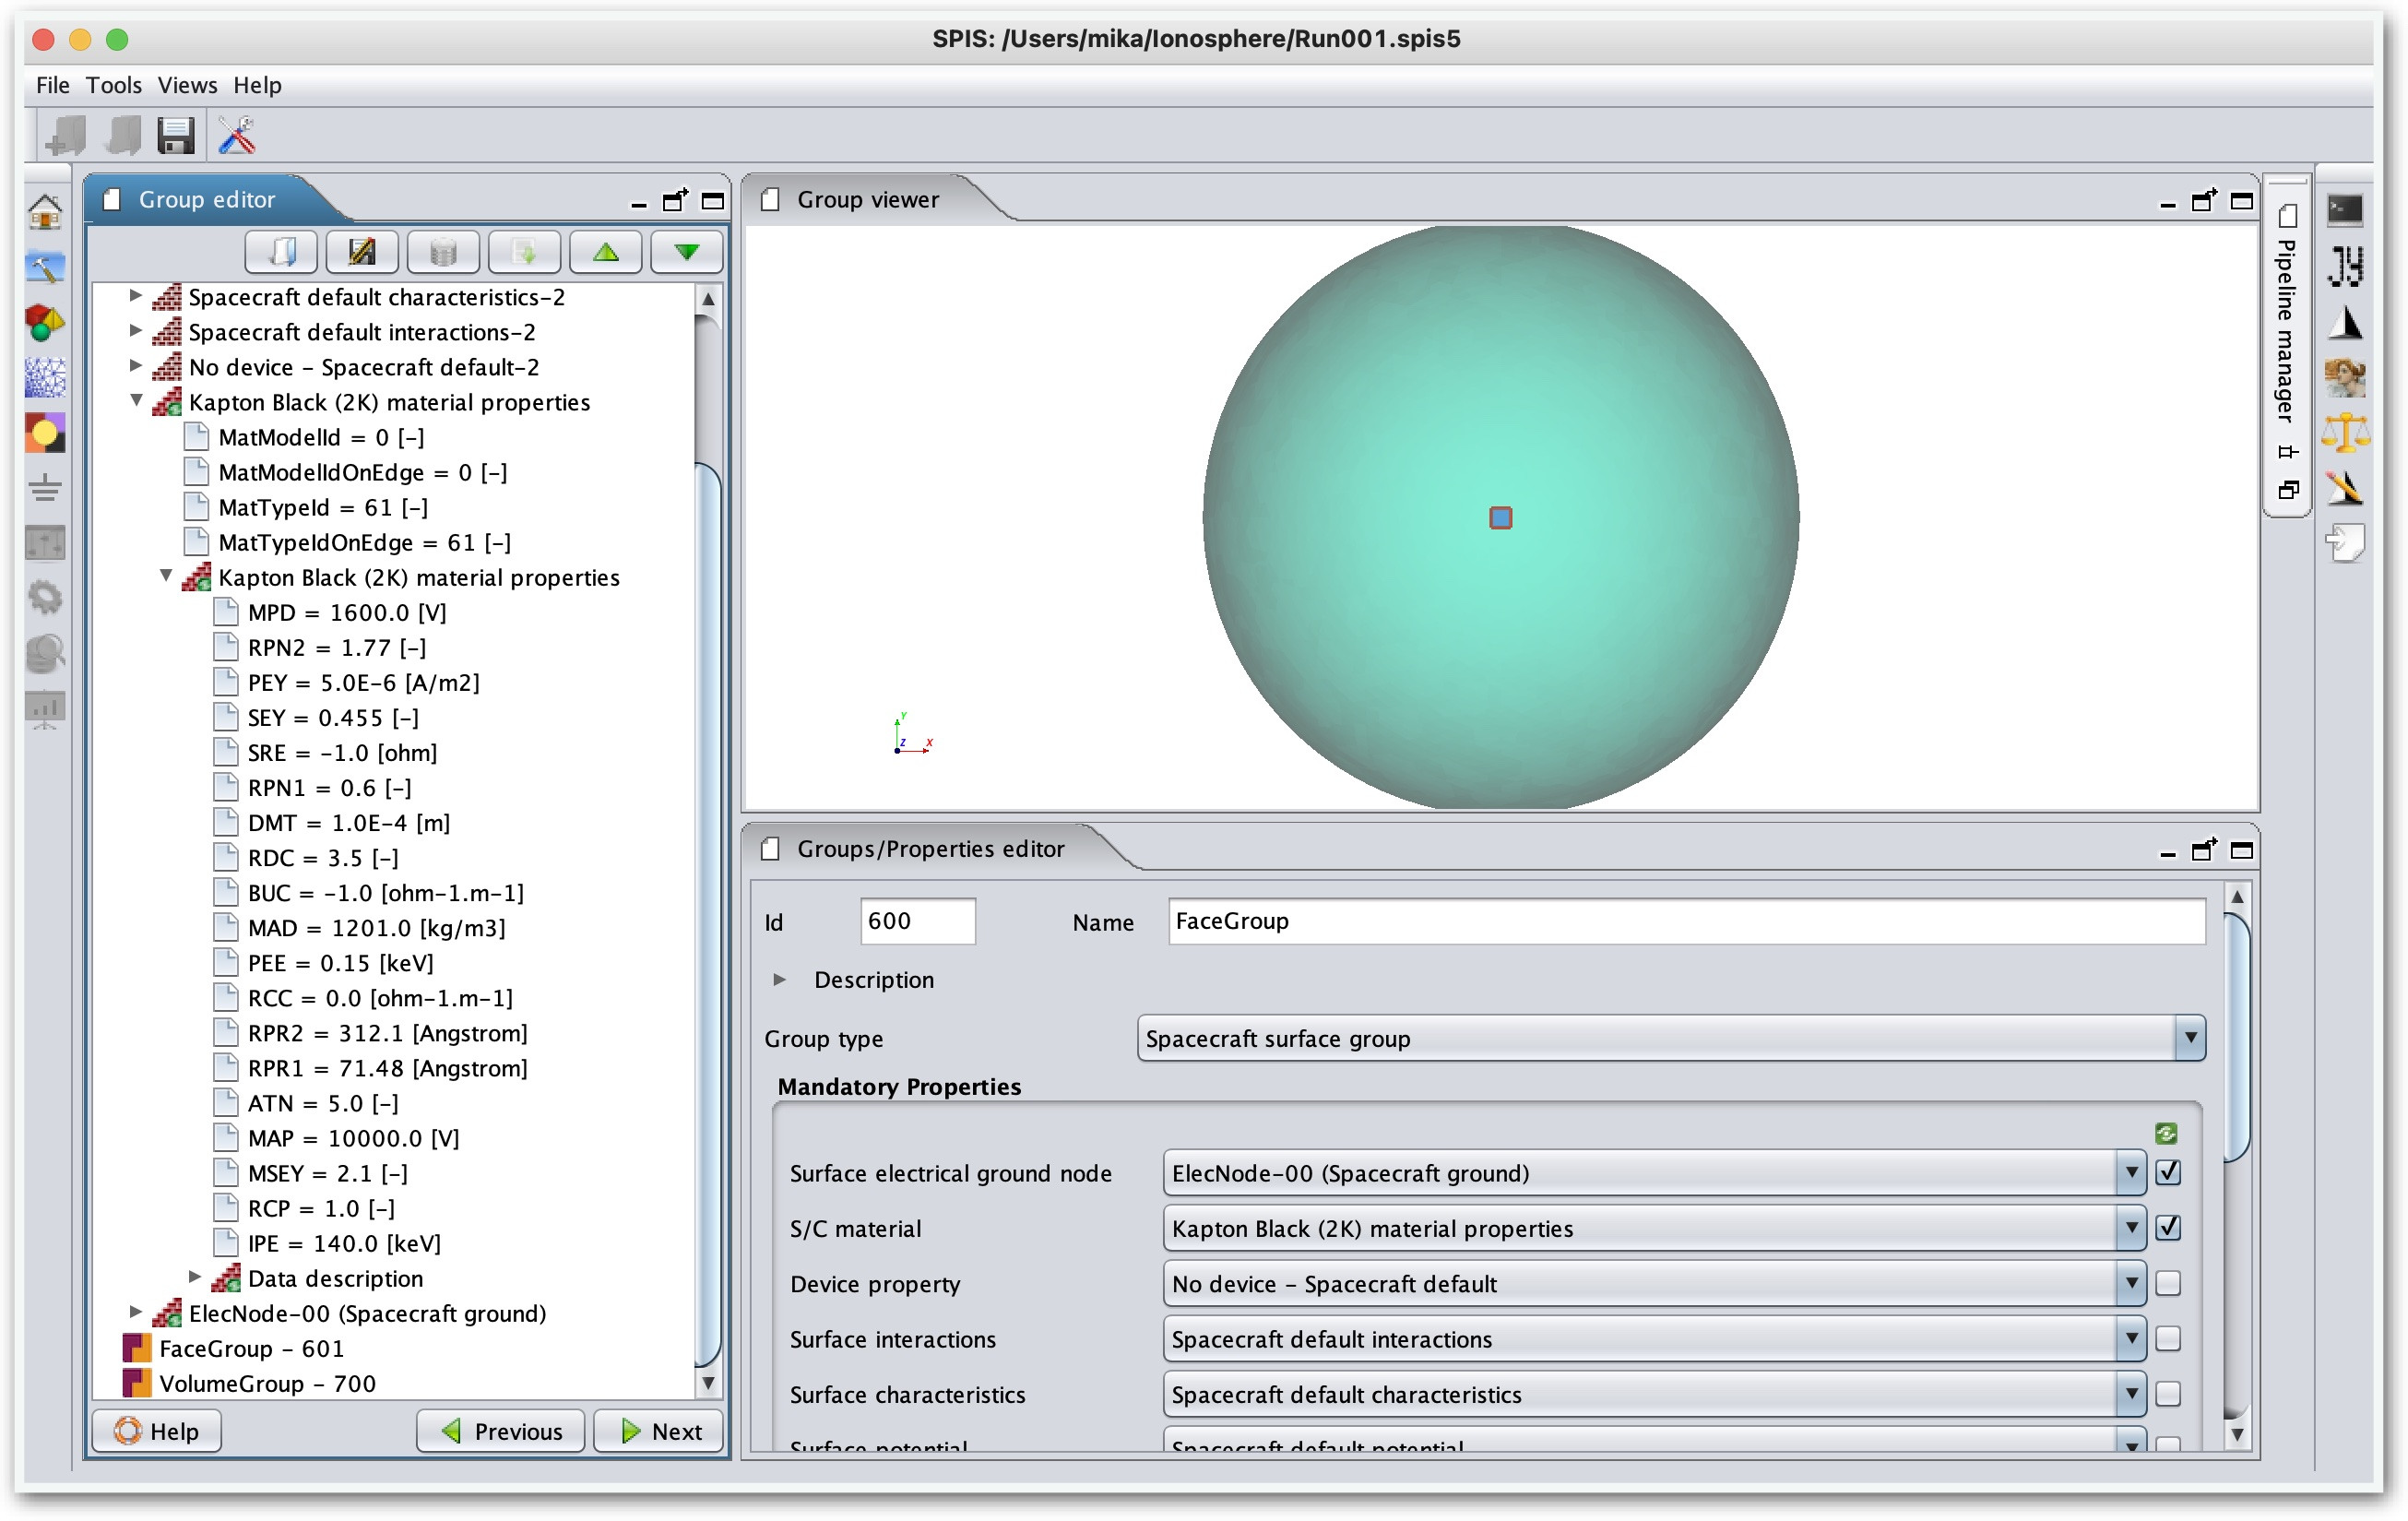
\includegraphics[width=0.45\textwidth]{fig13.jpg}
    \caption{The cross-section of the computational volume.}
\end{figure}

Figure 13 shows that no mesh elements are present inside the spacecraft, represented by the central square. If the spacecraft volume were not properly closed, mesh elements would also appear inside the spacecraft. Figure 13 also shows that the mesh elements are finer around the spacecraft, defined to be of the order of 0.1 m, and coarser at the outer boundary of the computational volume, where they are defined to be of the order of 2 m.\par
Once the mesh is finalised, it must be saved. Use "File", "Export", choose the file format "Mesh - Gmsh MSH (*.msh) and save the file in the preferred folder and with the preferred name, for example Spacecraft.msh. Click "Save", choose the "Version 2 ASCII" format and click "OK". The computational mesh is now ready to be used in SPIS simulations.

\subsection{Starting the SPIS simulation}

To start SPIS, open a terminal window, go to the SPIS folder and type "sh Spis.sh" or, in Windows, "Spis.bat". This should open a window like the one shown in Figure 14. To find the SPIS folder use the command "ls" to display the contents of the current directory and use the command "cd" to move to a different folder. For example, typing "ls" shows that the current location is the "mika" directory. The command "cd ../../" is then used to move two directories up to access the "Applications" folder and the SPIS folder named "SPIS-6.1.0-osx64b". The example is shown in Figure 15.

\begin{figure}[!ht]
    \centering
    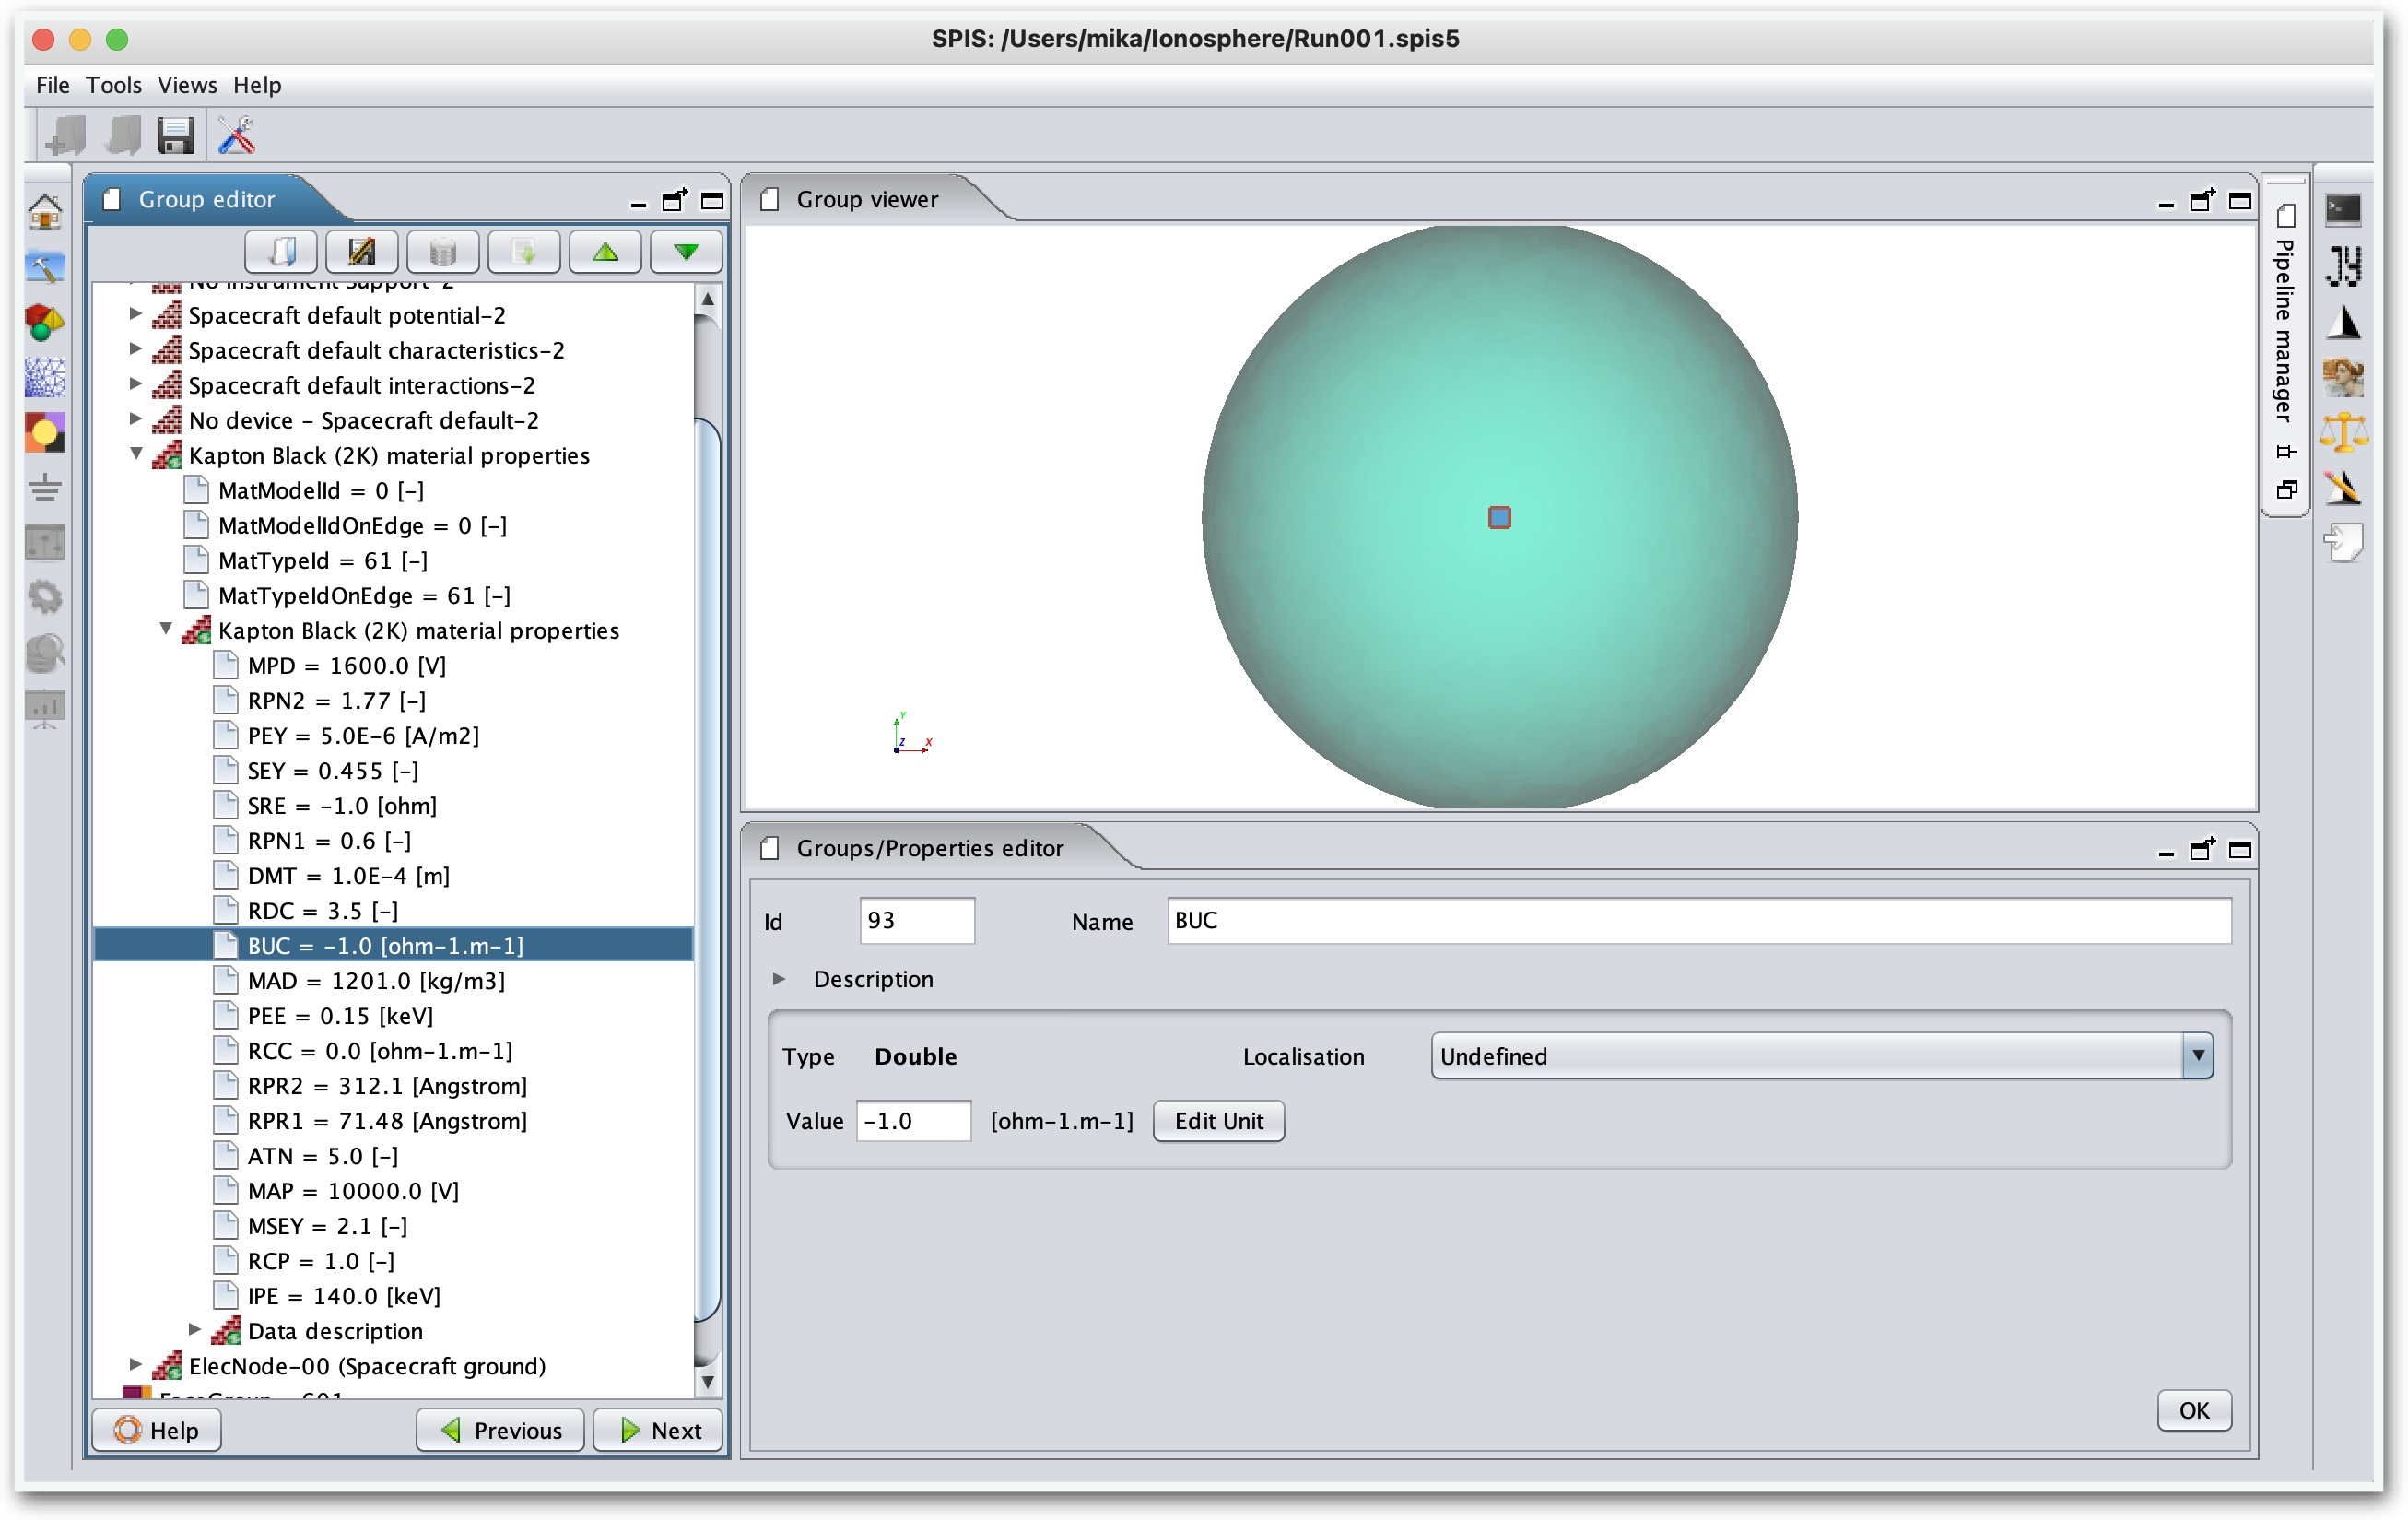
\includegraphics[width=0.45\textwidth]{fig14.jpg}
    \caption{The start of page SPIS.}
\end{figure}

\begin{figure}[!ht]
    \centering
    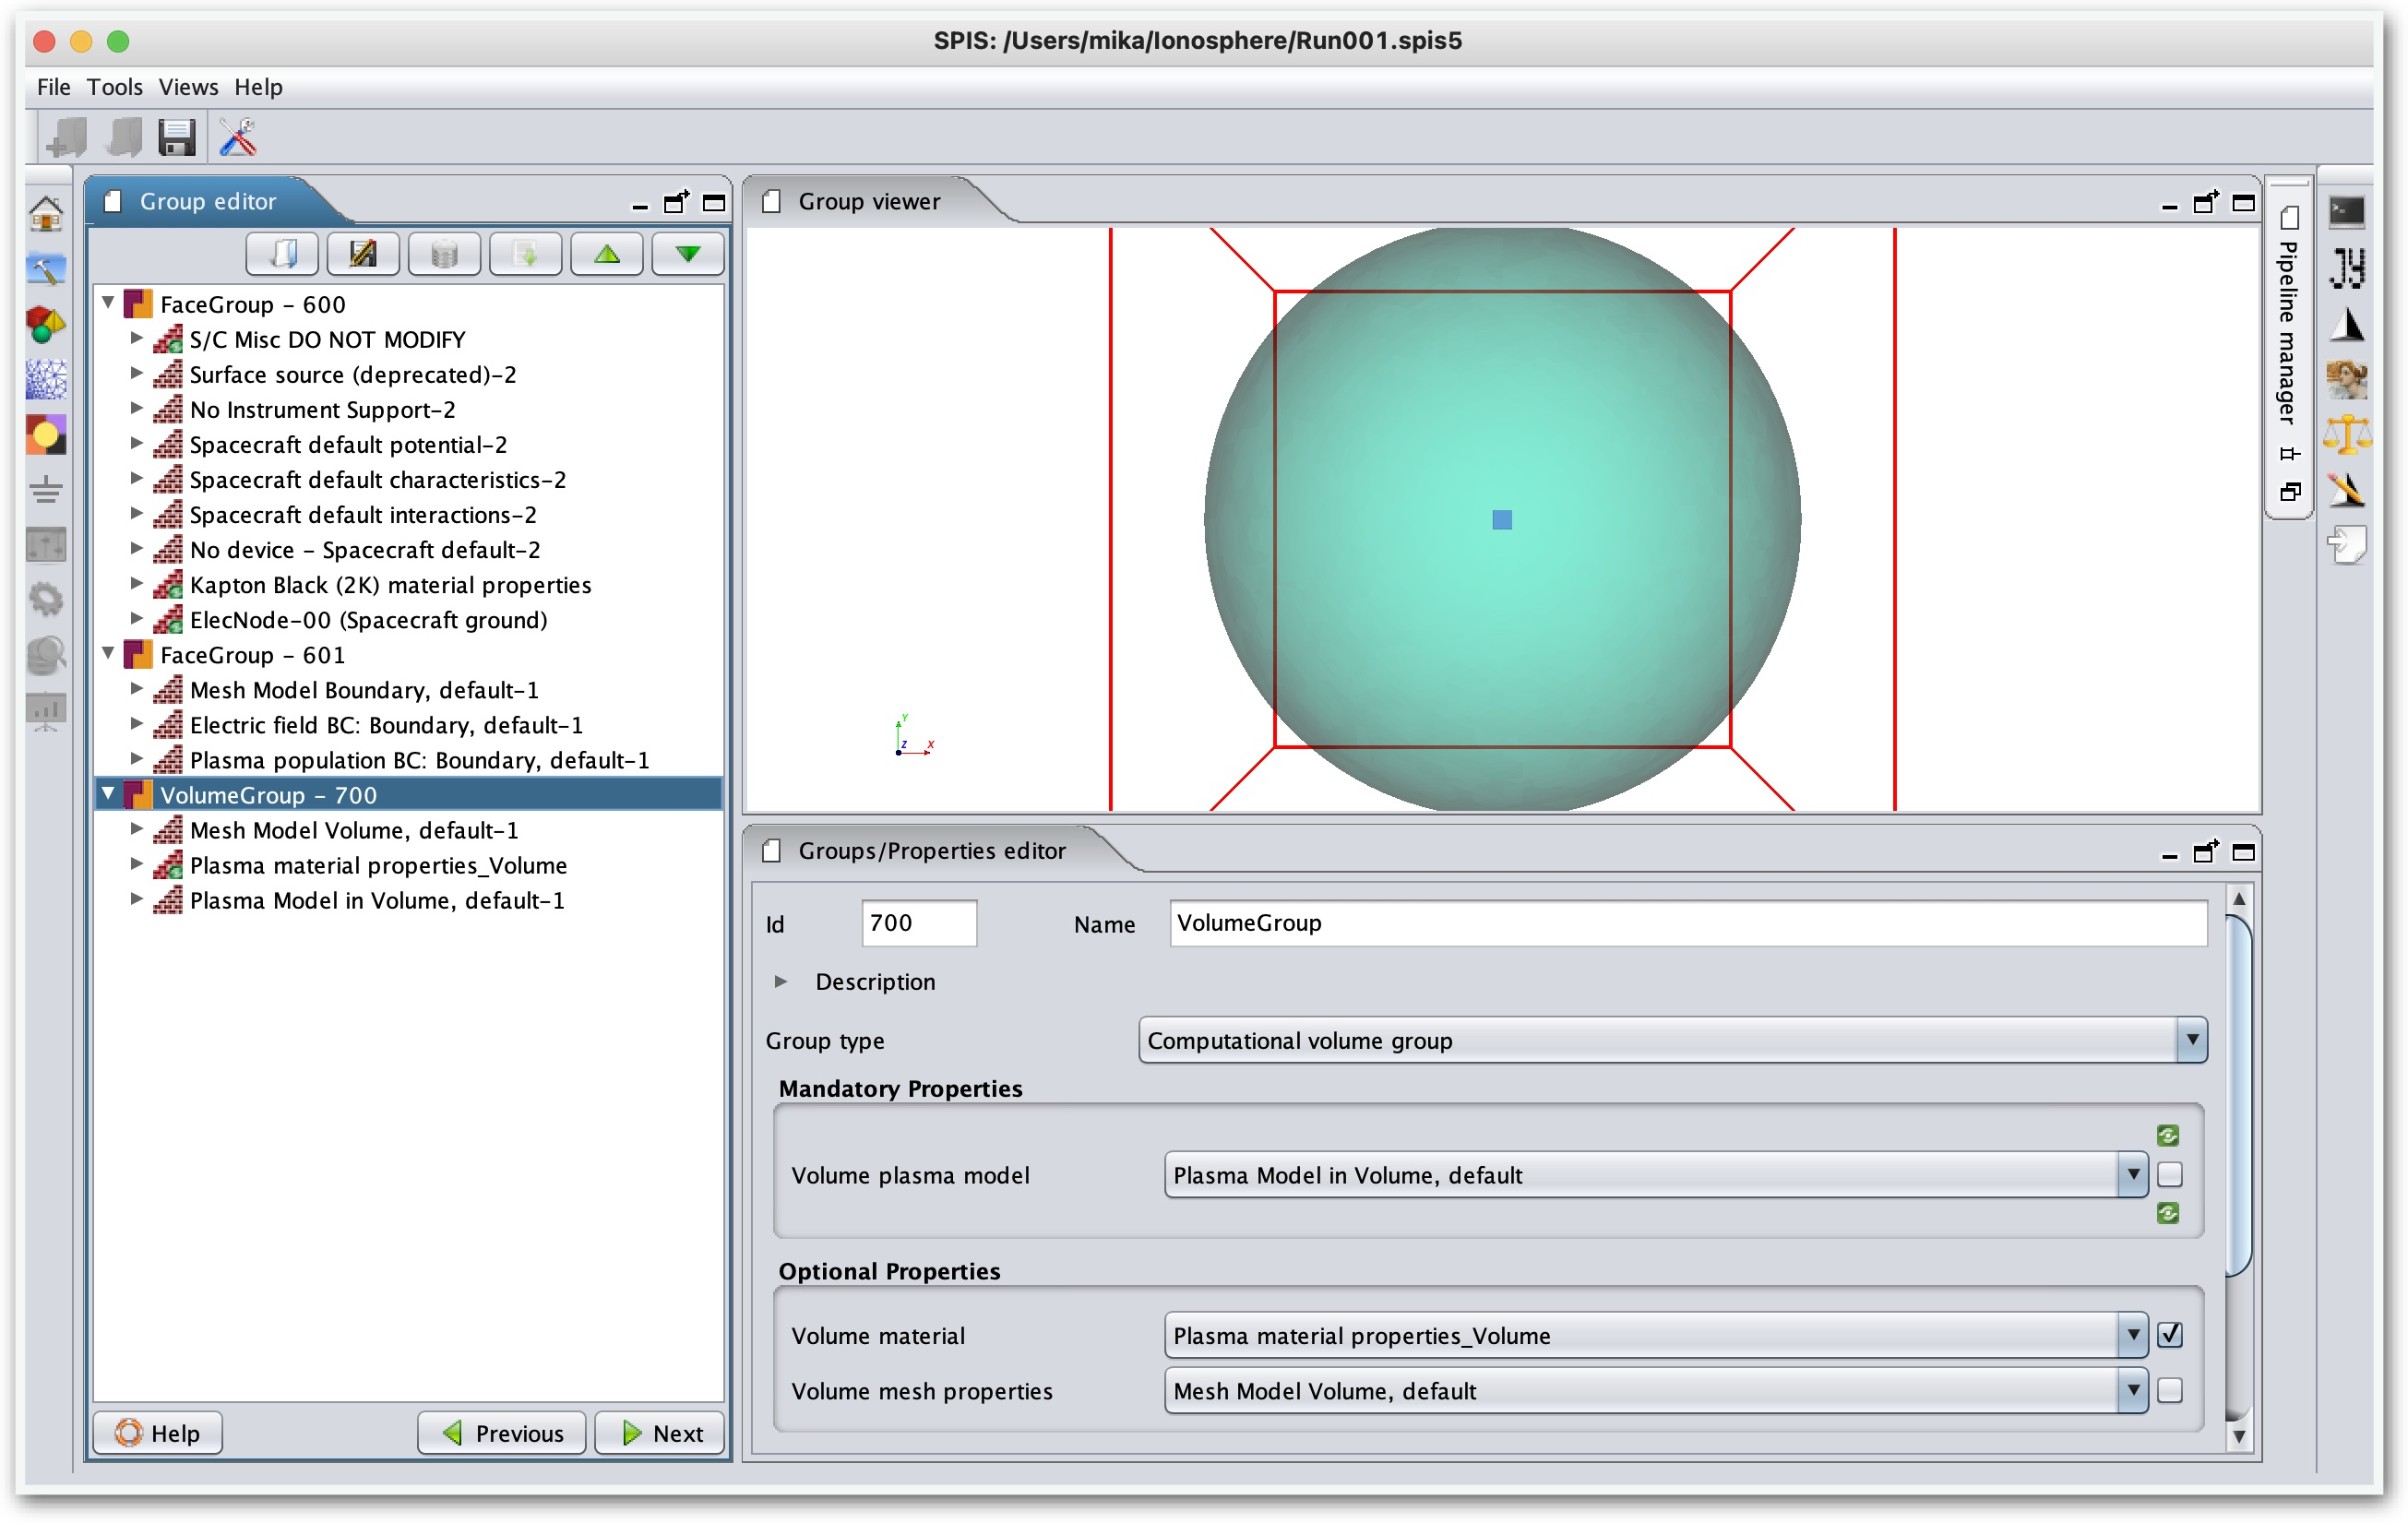
\includegraphics[width=0.45\textwidth]{fig15.jpg}
    \caption{How to navigate the SPIS folder.}
\end{figure}

For Mac users, the first attempt to open SPIS typically results in an error message. This is due to the default security settings of Mac, which only allows apps from App Store or from known developers to be opened. To change these settings go to "Security \& Privacy" setting in "System Preferences". This should open a window like the one shown in Figure 16. Make sure that "App Store and identified developers" is selected . Next to the blocked app, choose "Allow Anyway" and try to open SPIS again. This process will likely have to be repeated multiple times before the SPIS start window, like the one shown in Figure 14, will be opened. The main features from the SPIS start window are "Open an existing project", used to access previously started projects, and "Create a new project". Select "Create a new project" to begin.

\begin{figure}[!ht]
    \centering
    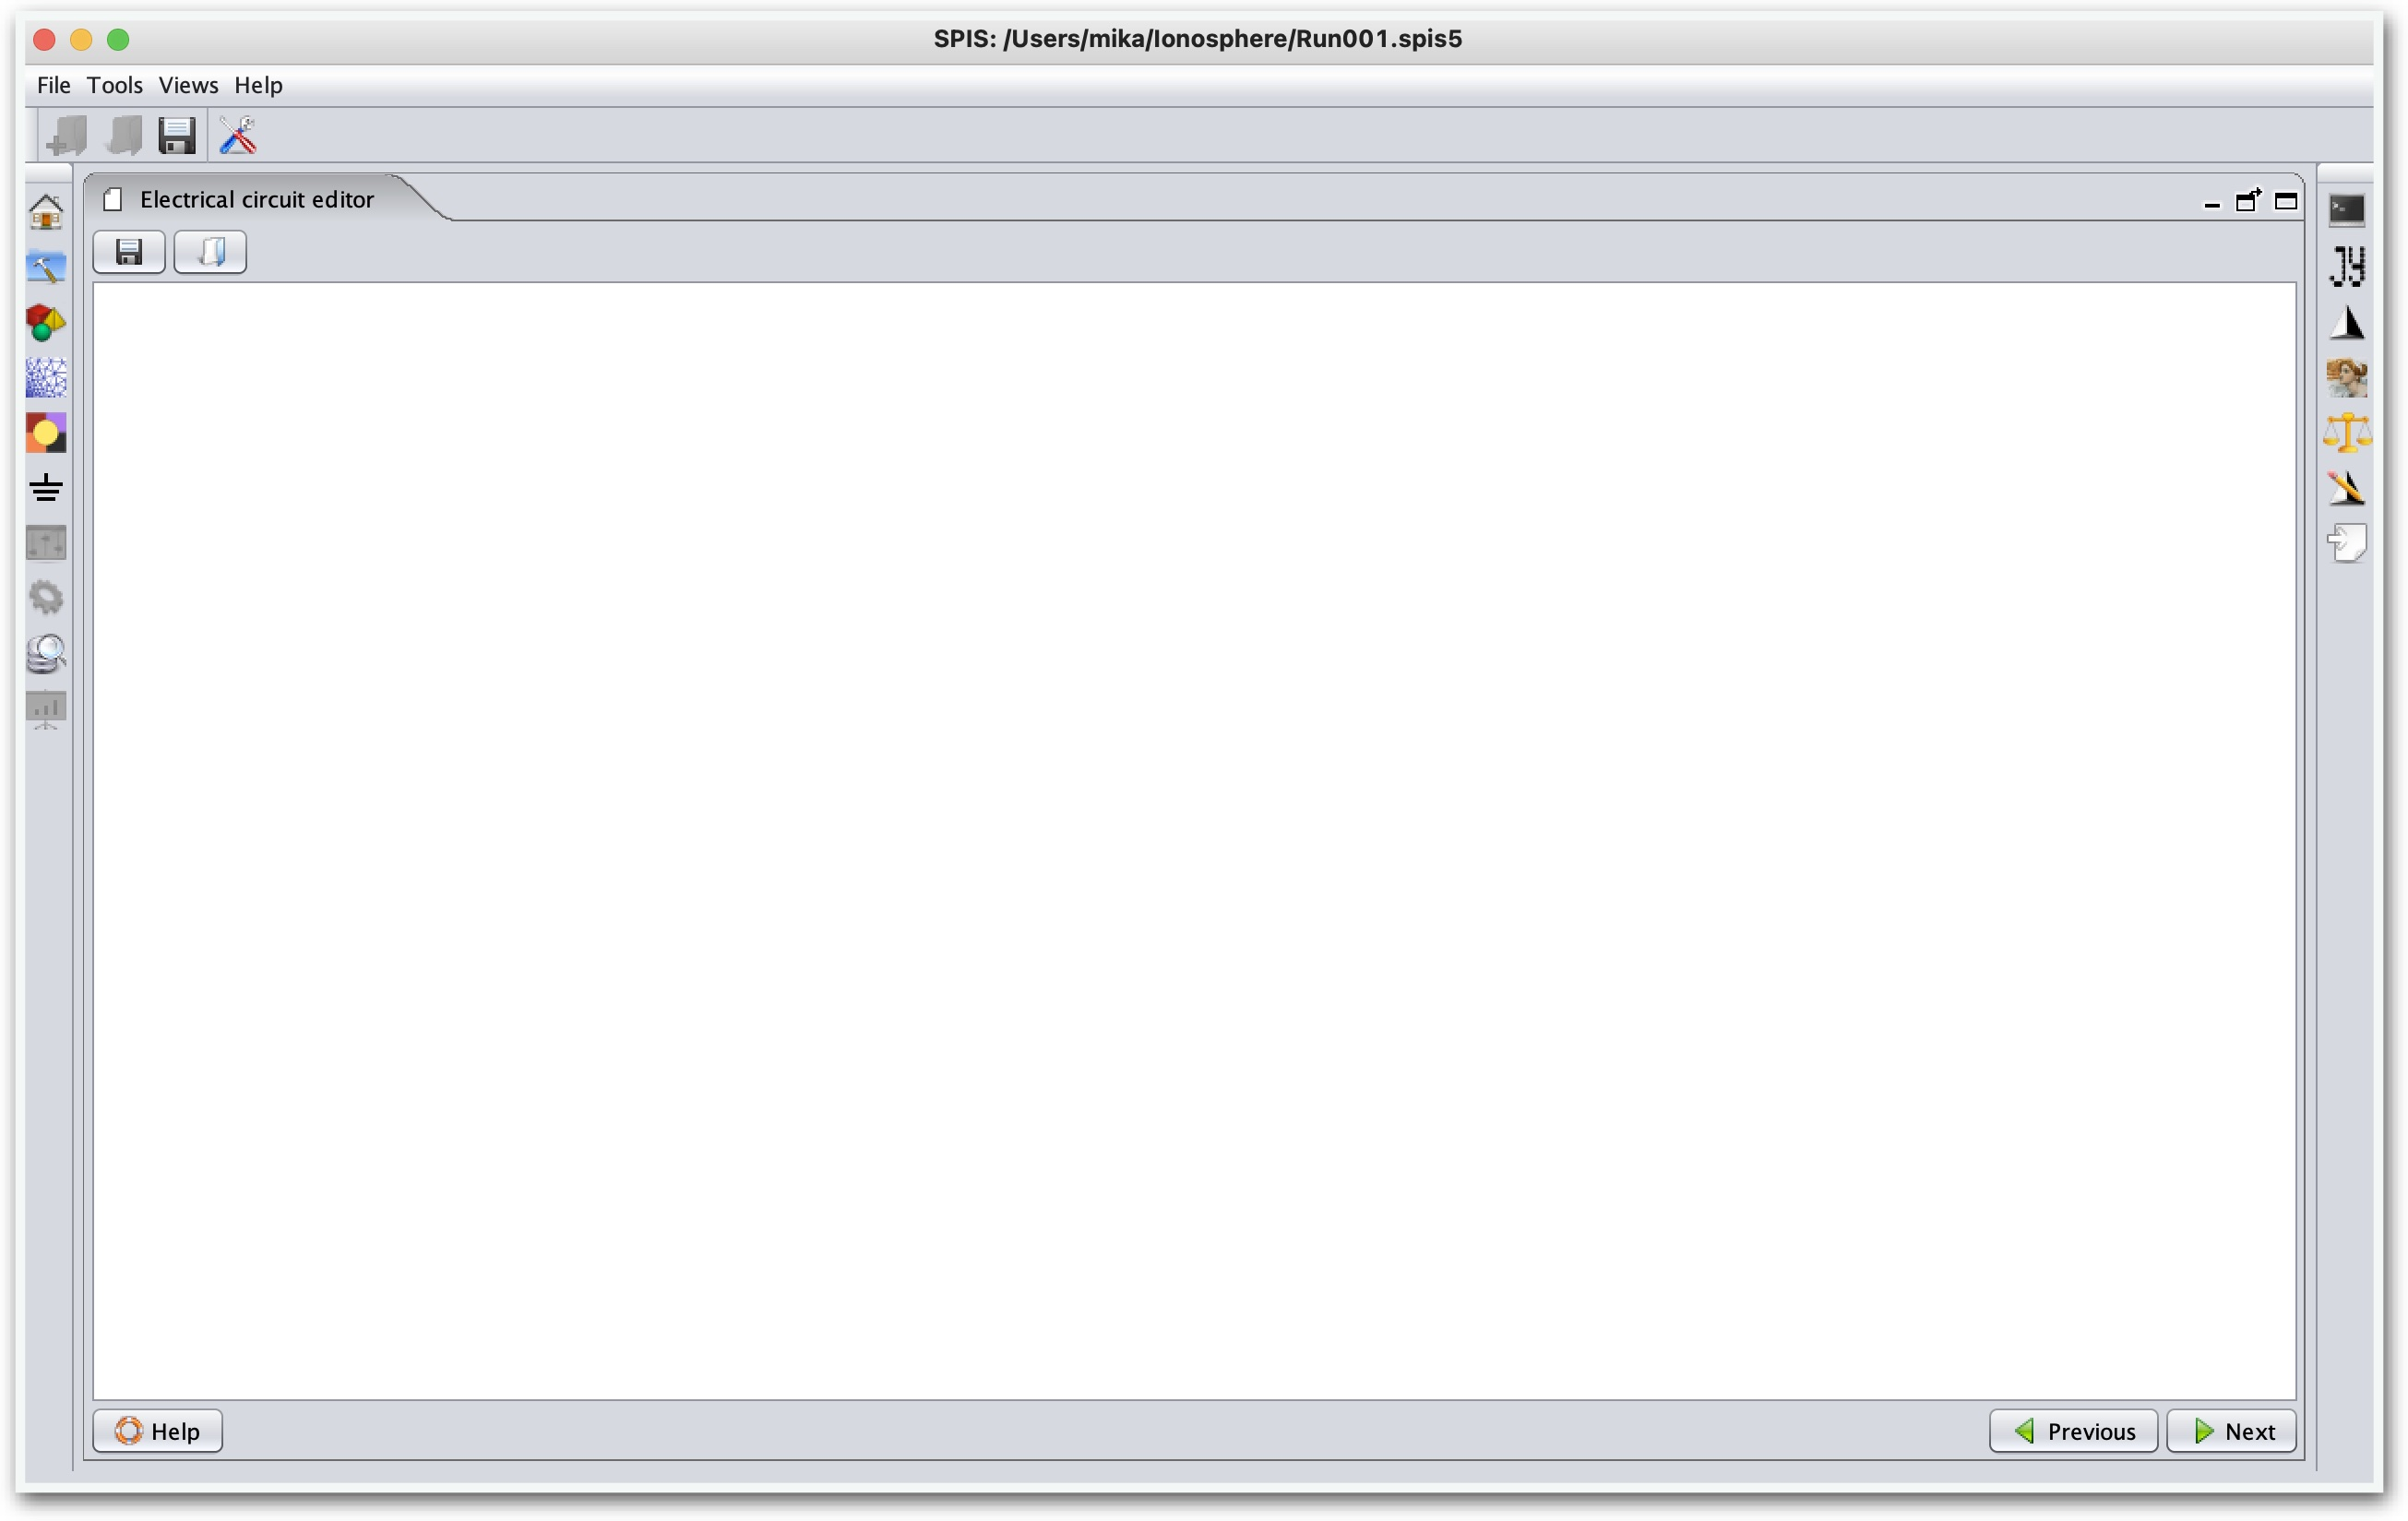
\includegraphics[width=0.45\textwidth]{fig16.jpg}
    \caption{Example of files included in the SPIS download that might have to be manually approved.}
\end{figure}

Clicking "Create a new project" opens the window shown in Figure 17, where a name for the new project must be specified. As multiple simulations with similar set-ups are likely to be executed, it is recommended to use a naming convention such as Run001. Including the 00 ensures that the projects are sorted in the correct order and not in, for example, the order Run1, Run100, Run2 etc. Select a "Project parent folder" that reflects the simulated environment or specific conditions, for example "Ionosphere". Since a large number of simulations are typically conducted during the course of a project, it is advisable to create a Readme document to log all the input parameters for each simulation. This will make it much easier to know what separates the different simulation runs. It is not advisable to try to list this in the name of the project, since this will lead to excessively long names that still fail to capture all the input parameters in the name.

\begin{figure}[!ht]
    \centering
    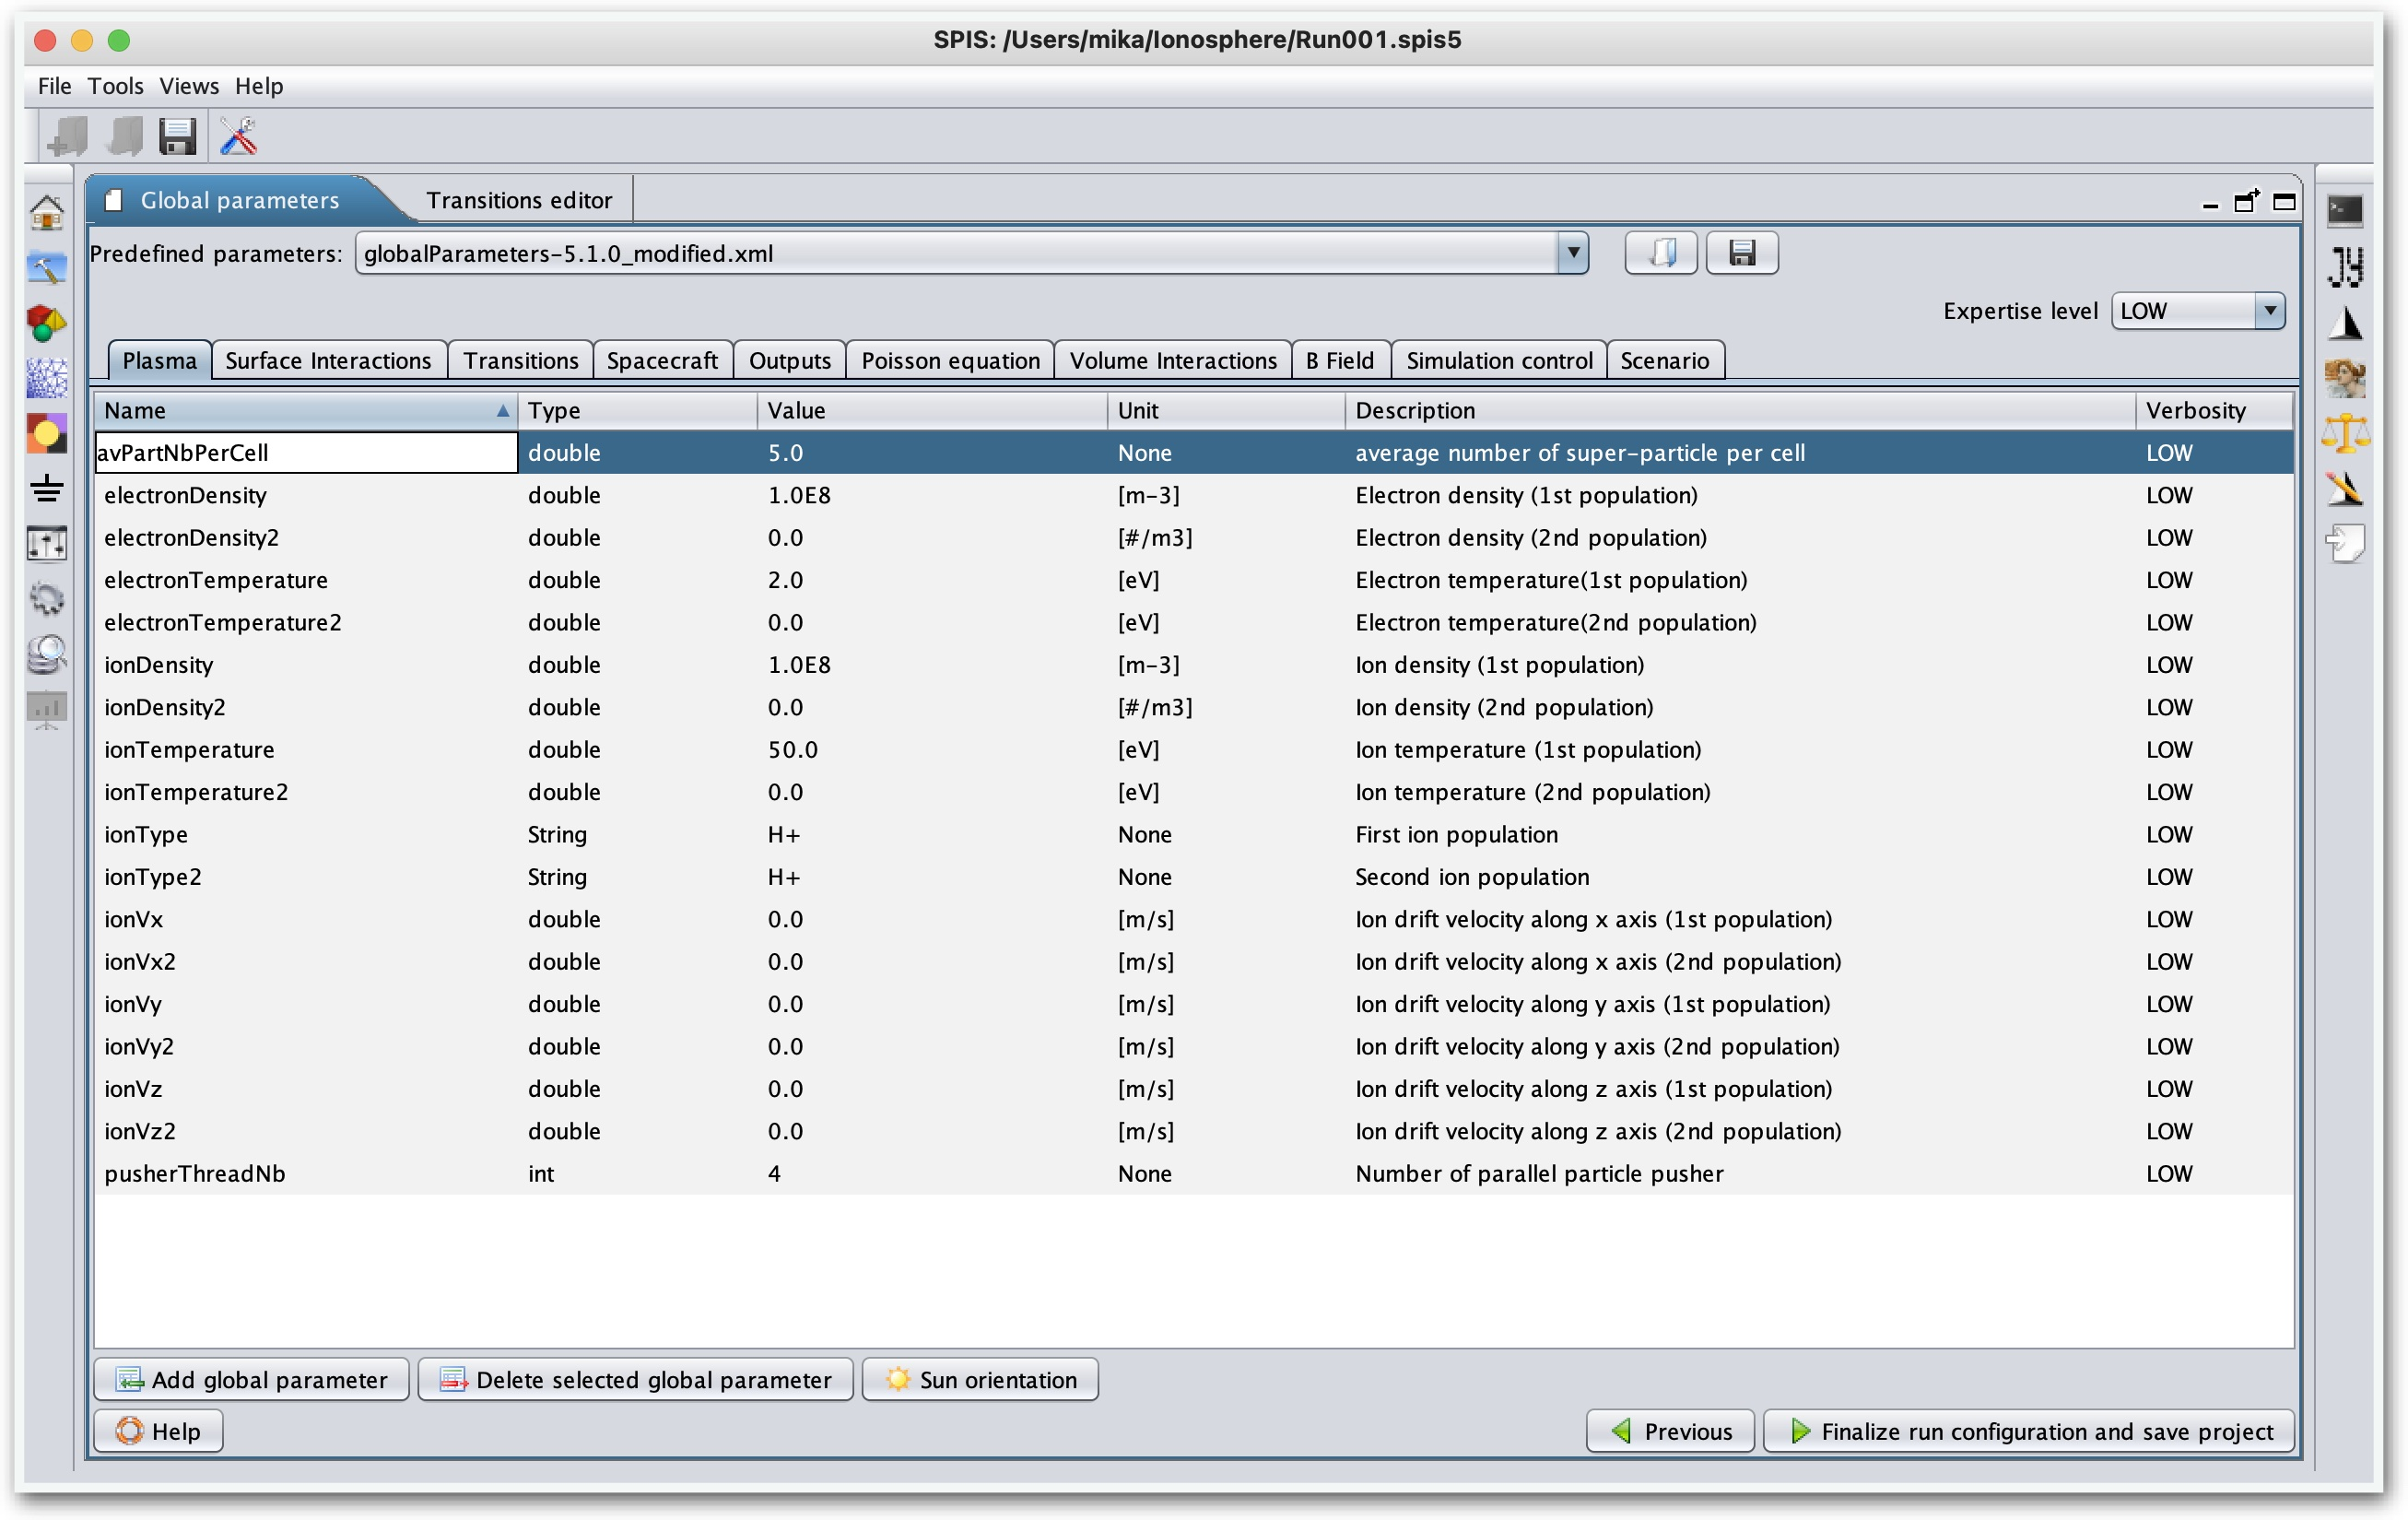
\includegraphics[width=0.45\textwidth]{fig17.jpg}
    \caption{Name your project and place it in the correct folder.}
\end{figure}

Since the mesh has already been created using Gmsh, this step can be skipped by selecting the "Skip geometry editor" option. Click "Create project and save" and you have now started your first SPIS project. Congratulations! The next window looks like the one in Figure 18 and this is the point at which the spacecraft model construction begins.

\begin{figure}[!ht]
    \centering
    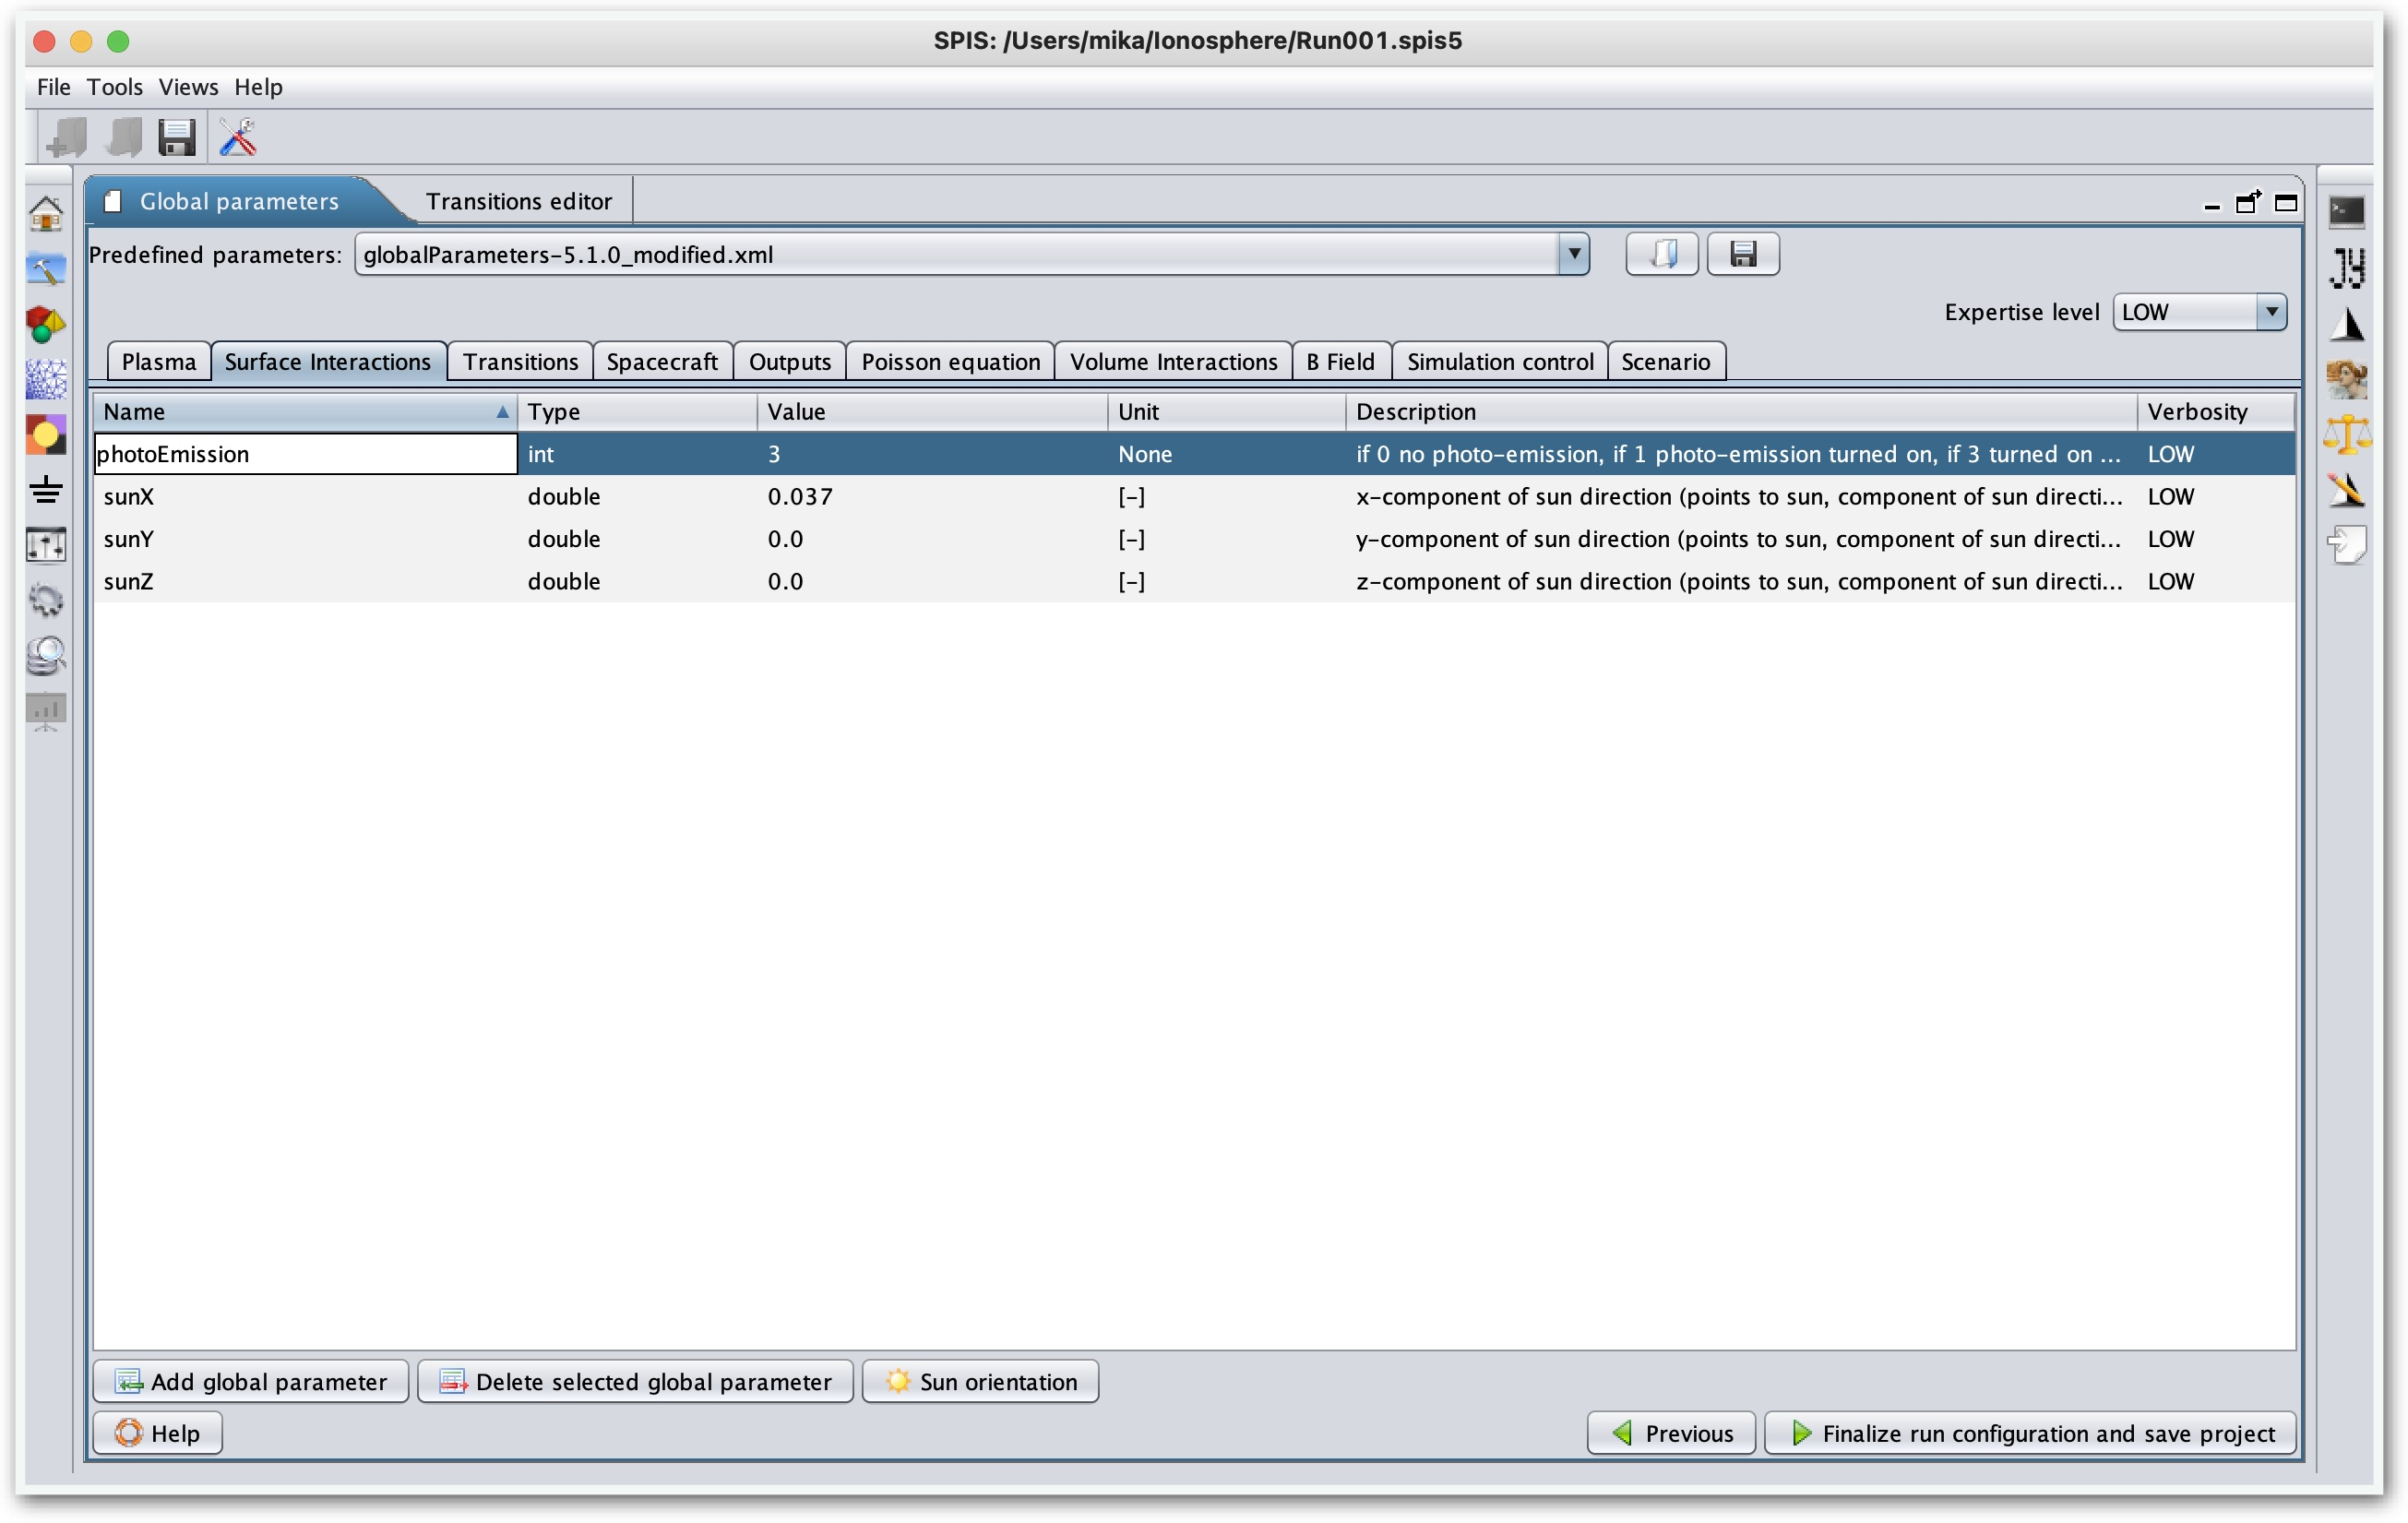
\includegraphics[width=0.45\textwidth]{fig18.jpg}
    \caption{The SPIS spacecraft geometry window.}
\end{figure}

\subsection{The material library} %unclear how to import mesh if already generated, and how to get to figure 20

The next step is to define the properties of the spacecraft materials using the group editor, as shown in Figure 19. In the left menu, all defined physical surfaces and volumes will appear. They are identified with the assigned ID numbers. The first physical surface is the spacecraft with ID number 600. Selecting this surface allows the "Group type" to be set, which should be "Spacecraft surface group". This group type includes a range of properties, most of them can be left at their default values, but the most important one is the "S/C material". SPIS already has a material library with many common spacecraft materials, for this example the "Kapton Black (2K) material properties" is selected, which is a common spacecraft surface material.

\begin{figure}[!ht]
    \centering
    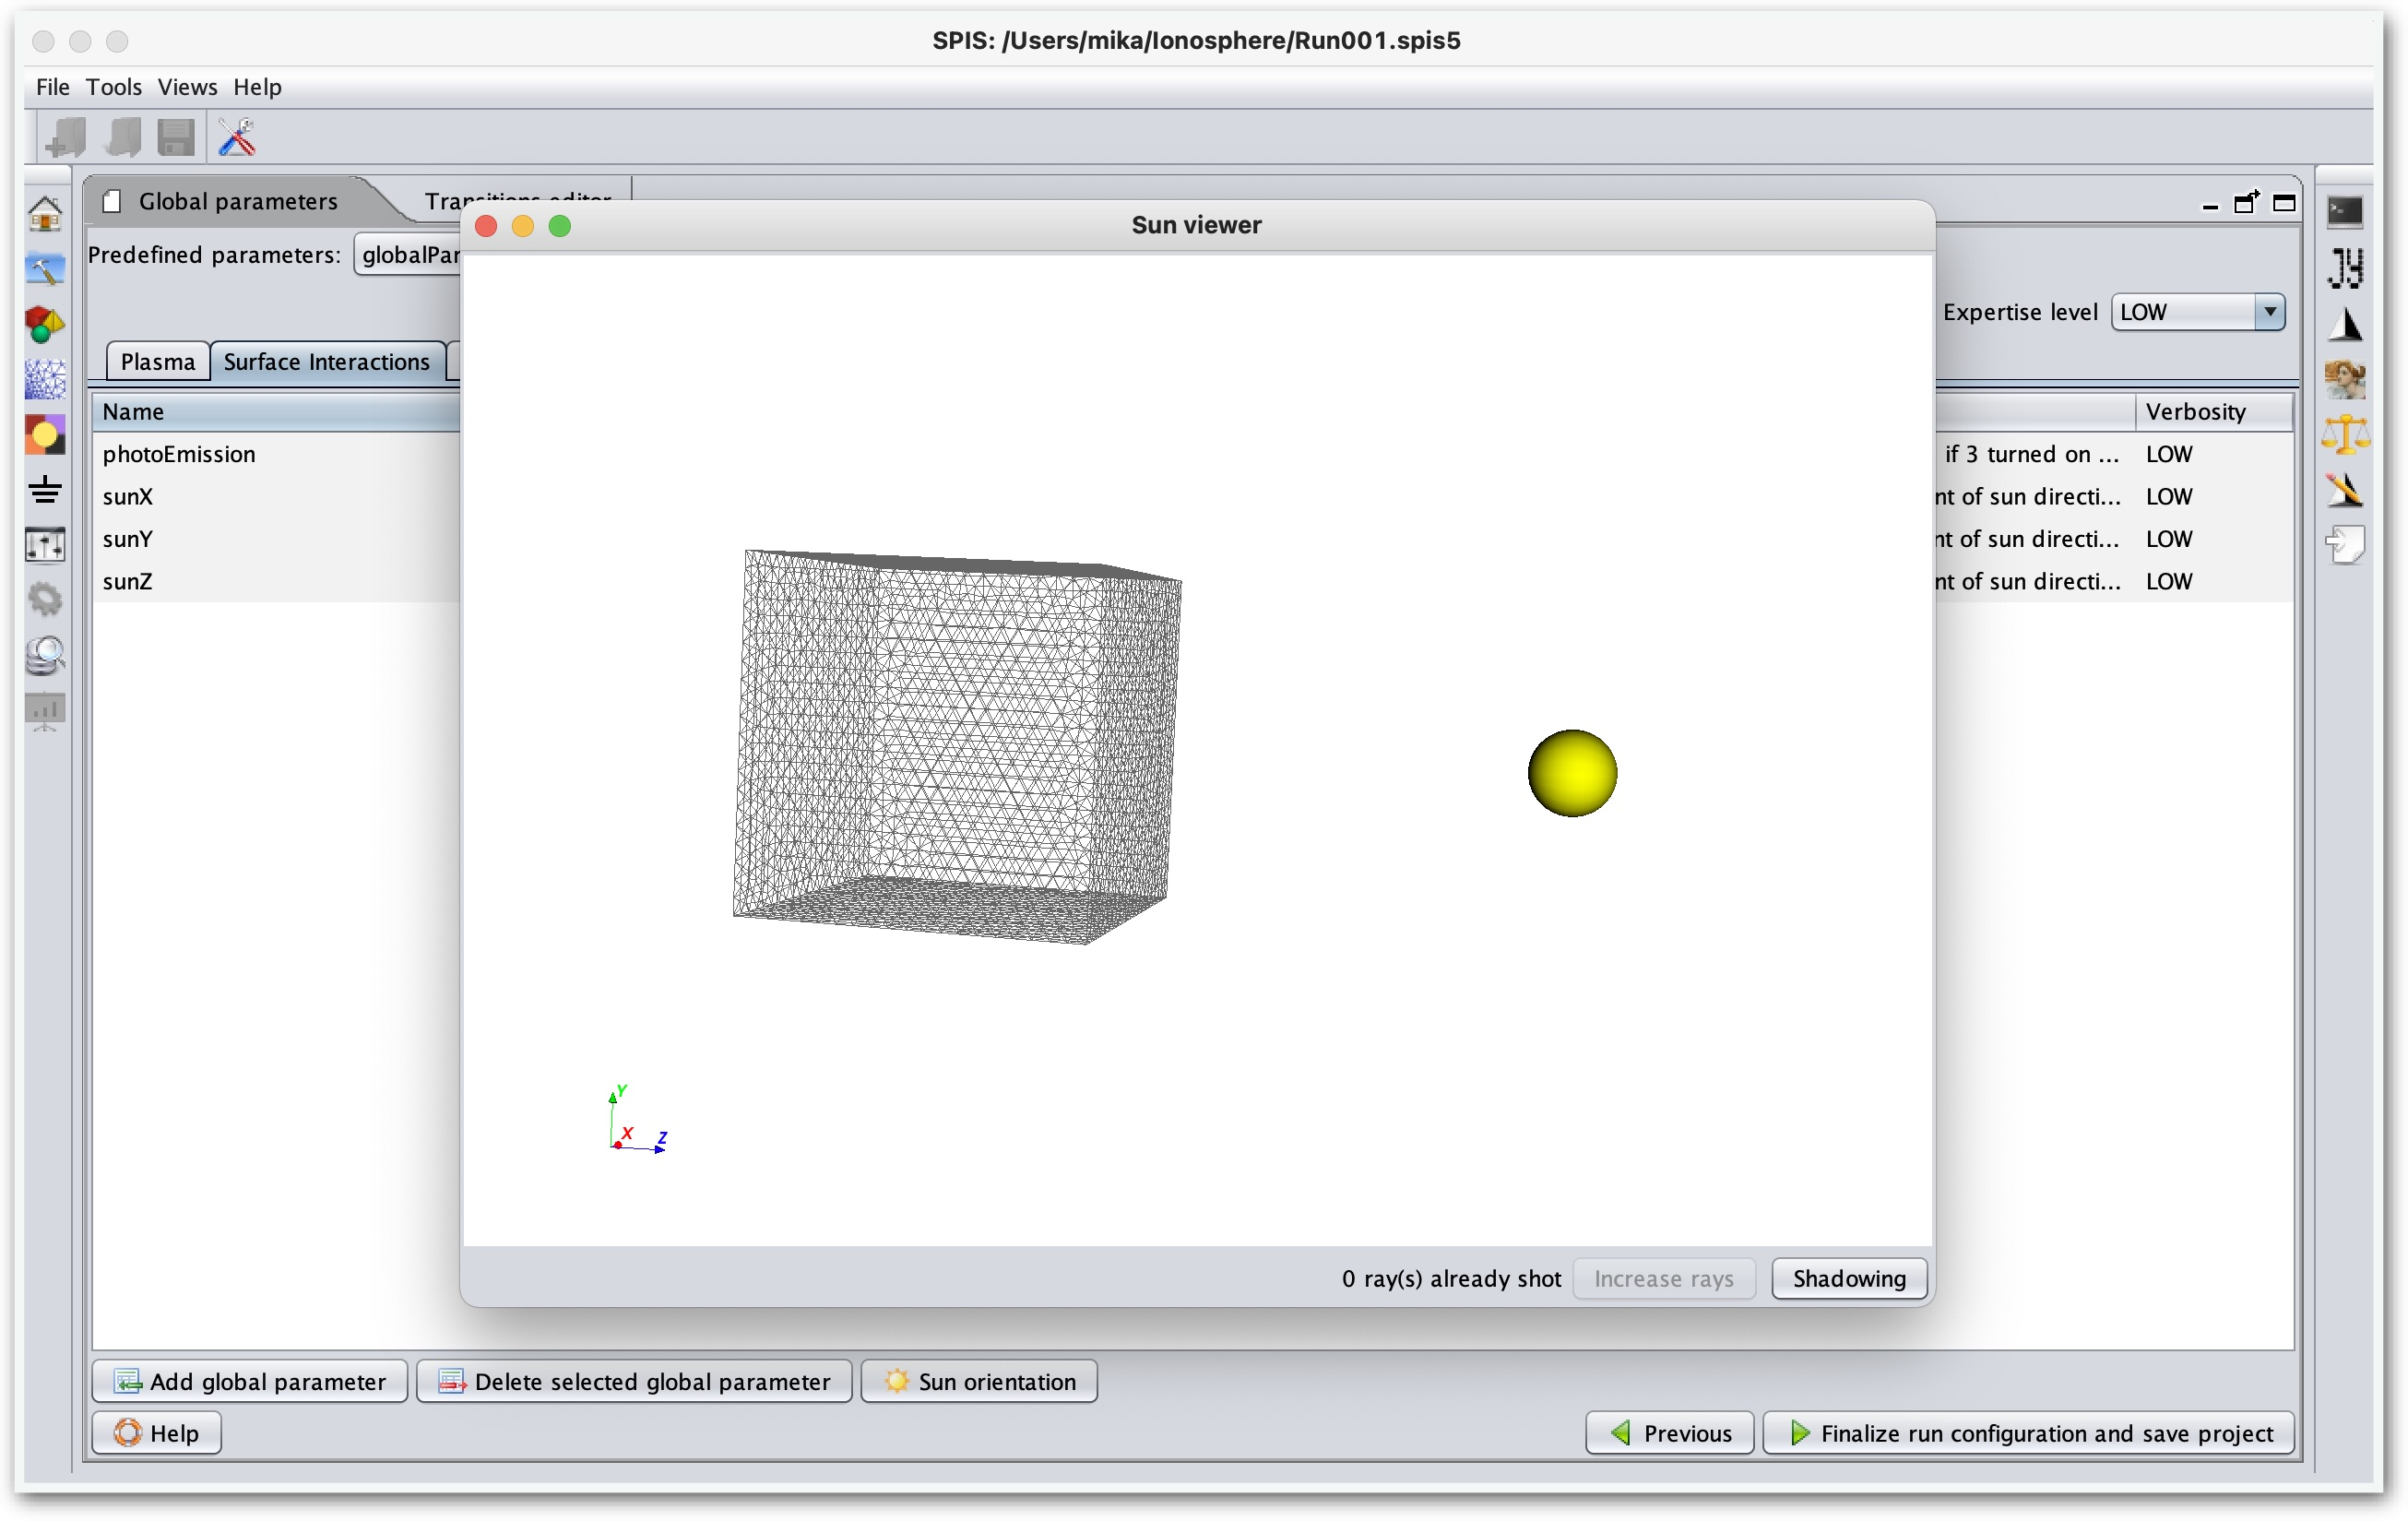
\includegraphics[width=0.45\textwidth]{fig19.jpg}
    \caption{The group editor where the material properties are defined.}
\end{figure}

Select the surface material and click "OK". The different material properties will then be added to this specific surface as shown in Figure 20. When "Kapton Black (2K) material properties" is selected and expanded, a list of associated properties appears, as shown in Figure 21. These properties can be modified if needed. The definition of the different properties are listed in Appendix B. For example, to explore how the spacecraft charging will change with a less conductive version of black kapton, the bulk conductivity parameter called BUC can be adjusted. For black kapton this value is set to -1, which means that it is simulated as a perfect conductor. To test an alternative conductivity value, click on the parameter "BUC" and change the value in the right window, as shown in Figure 22.

\begin{figure}[!ht]
    \centering
    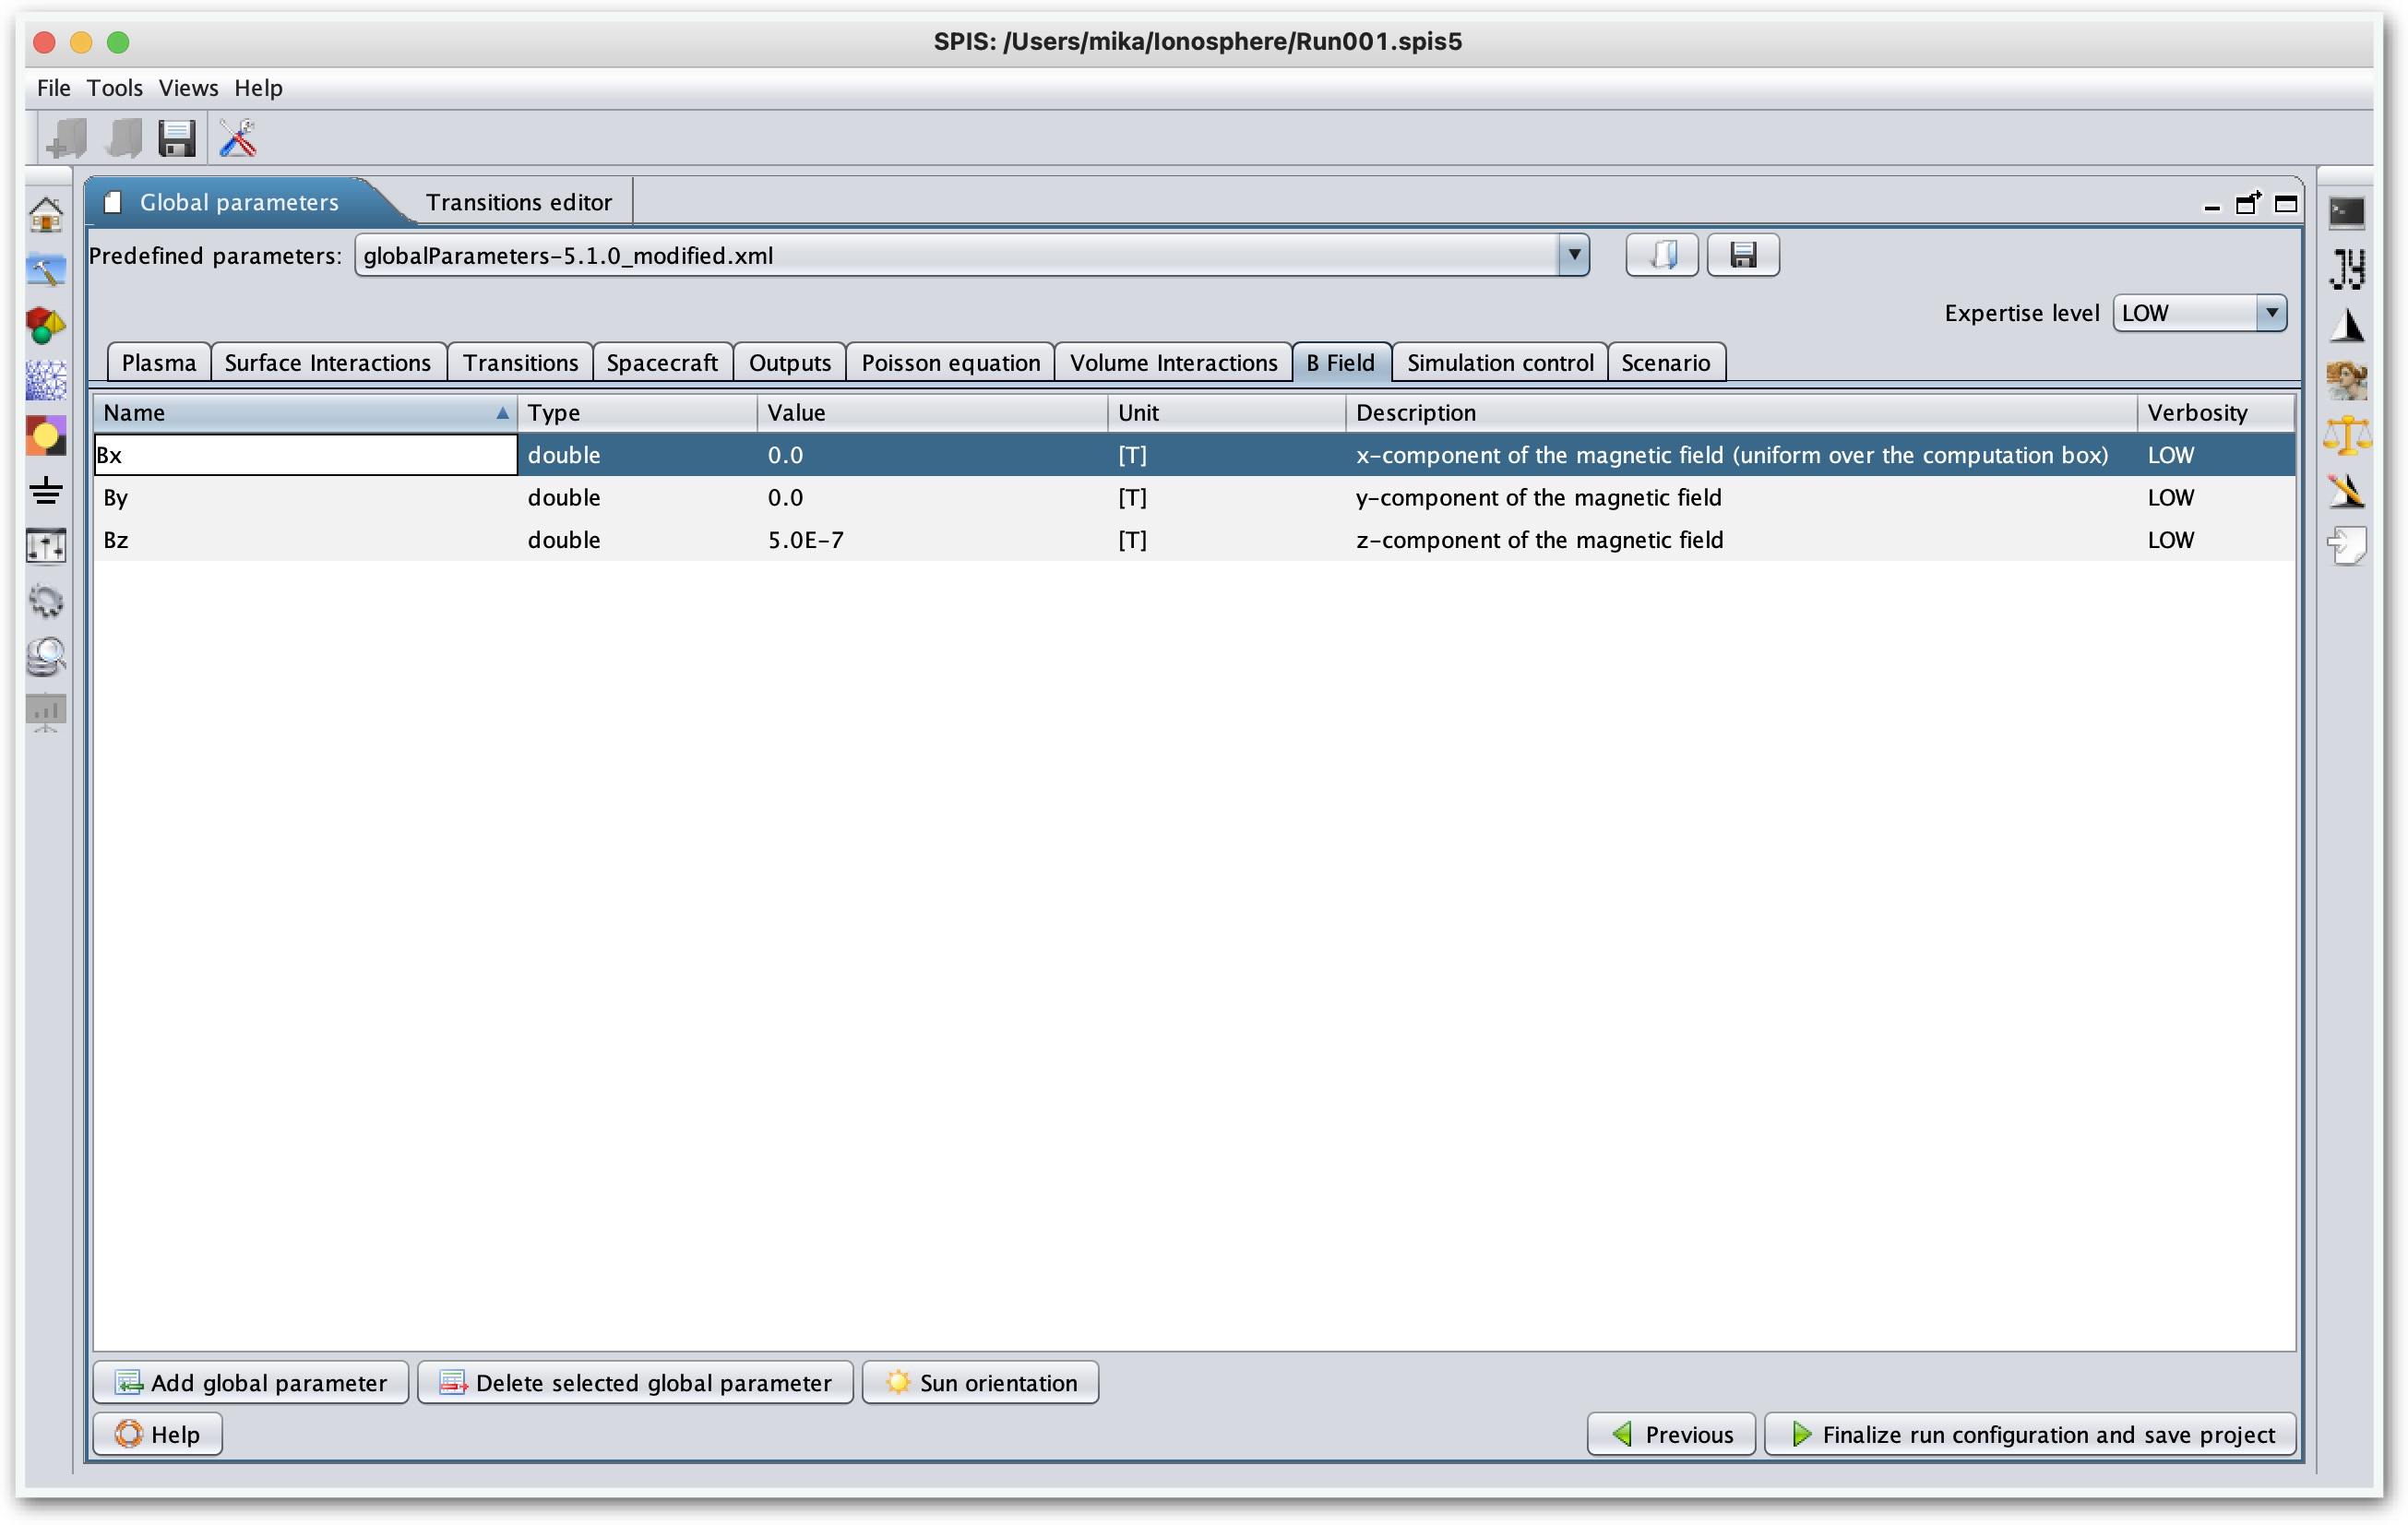
\includegraphics[width=0.45\textwidth]{fig20.jpg}
    \caption{Choose the spacecraft surface material.}
\end{figure}

\begin{figure}[!ht]
    \centering
    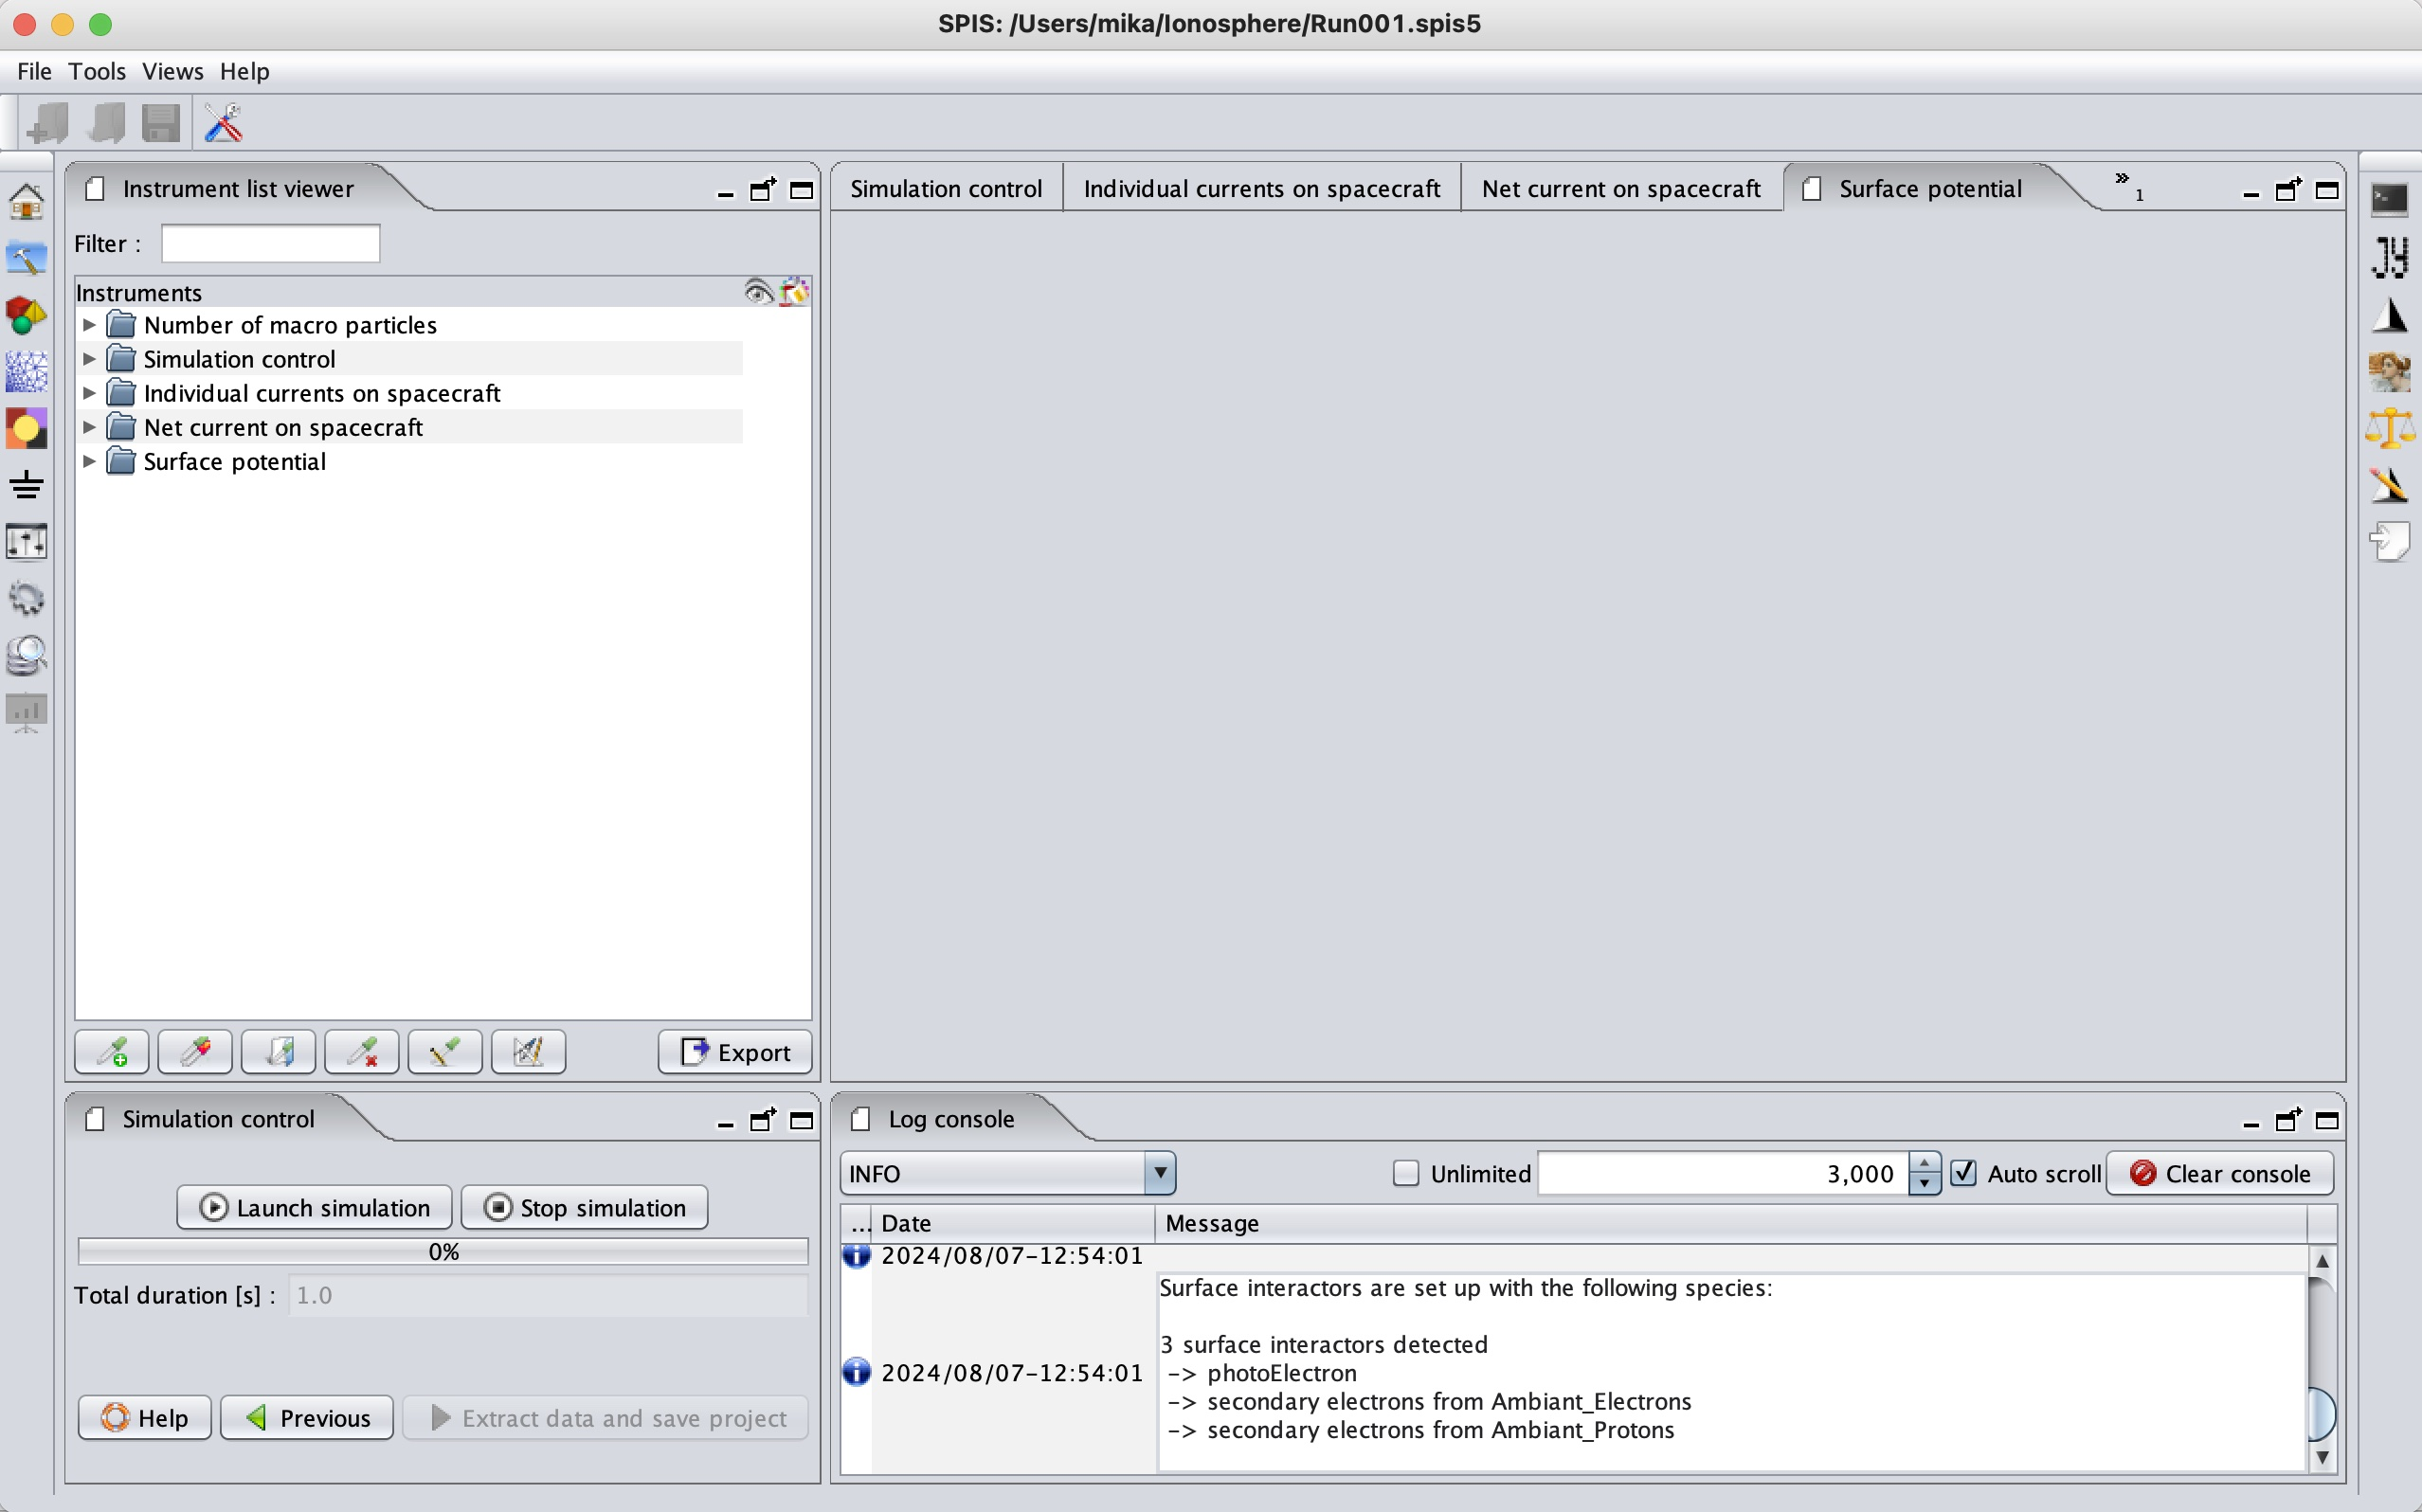
\includegraphics[width=0.45\textwidth]{fig21.jpg}
    \caption{The material properties are listed in the left menu.}
\end{figure}

\begin{figure}[!ht]
    \centering
    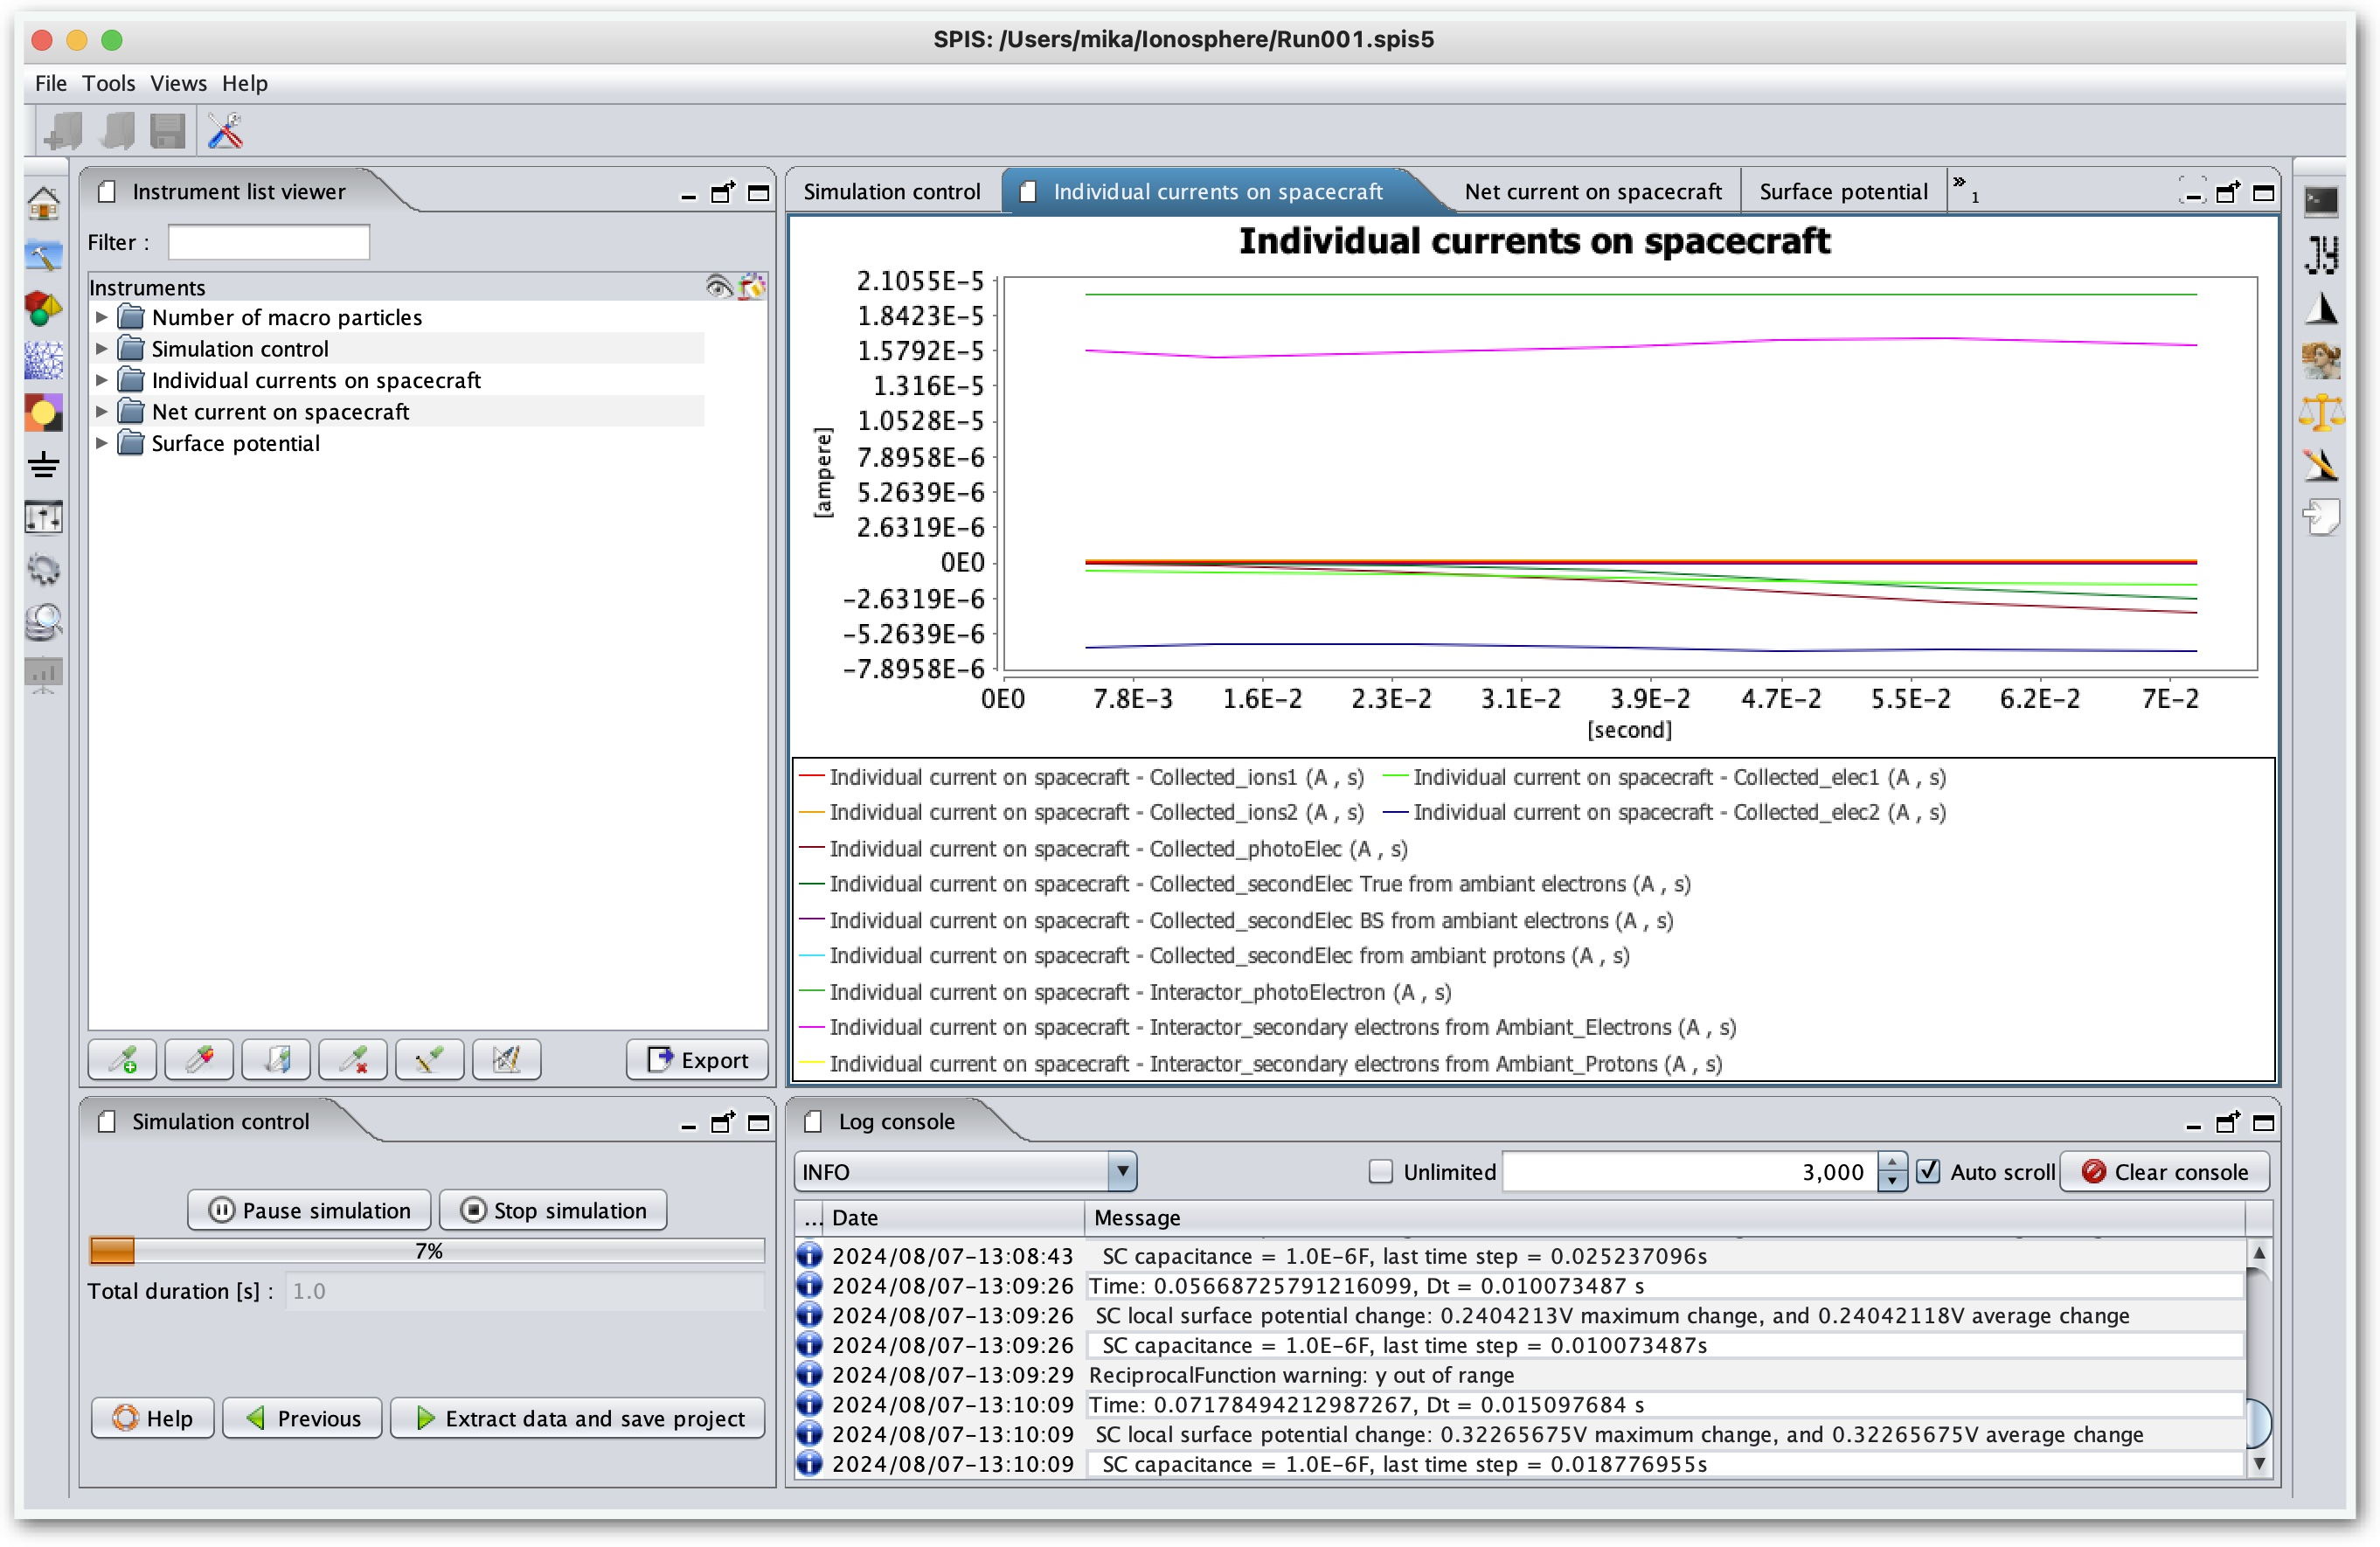
\includegraphics[width=0.45\textwidth]{fig22.jpg}
    \caption{To change a material property.}
\end{figure}

The next group is the external boundary with ID 601. Click on "FaceGroup - 601",  choose "External boundary group" and "OK". Then Click on "VolumeGroup -700", choose ""Computational volume group" and "OK". The group editor should then look like in Figure 23. Then click "Next".

\begin{figure}[!ht]
    \centering
    \includegraphics[width=0.45\textwidth]{fig23.jpg}
    \caption{The group editor after all groups have been defined.}
\end{figure}

\subsection{The circuitry}

The next step is to define the electrical circuit. This is where to specify how the various parts of the spacecraft are electrically connected. The different parts can be connected using resistors (called R), capacitors (C), or voltage generators (V). An example would be\par

V  0  1  -10
R  0  2  1.e6

which mean that a biased voltage of -10 V would be imposed between surface 0 and 1, and a resistor of 1.e6 Ohm is set between surface 0 and 2. Since we only have one spacecraft surface we can leave this section blank, as shown in Figure 24, and just press "Next".

\begin{figure}[!ht]
    \centering
    \includegraphics[width=0.45\textwidth]{fig24.jpg}
    \caption{The electric circuit editor.}
\end{figure}

\subsection{The environment}

The final step before starting the simulations is to define the environment in which the spacecraft is located. When issues arise during simulations, they are most often caused by poorly defined spacecraft geometry or mesh, or a badly defined environment. It is therefore especially important to have a solid understanding of the space environment of the spacecraft. Take the time to carefully review and double check all environmental parameters. If you are not an expert yourself, consult an expert to ensure that the parameters accurately represent the environment.\par
The window used to define the environmental parameters is named "Global parameters" and looks like the window shown in Figure 25.

\begin{figure}[!ht]
    \centering
    \includegraphics[width=0.45\textwidth]{fig25.jpg}
    \caption{Here you define your spacecraft environment.}
\end{figure}

If more parameters are displayed than those shown in Figure 25, then change the "Expertise level" to "LOW". These are the initial parameters to be configured. The different options are "Plasma", "Surface Interaction", "Transitions" etc. Begin by defining the plasma environment. Set the electron and ion densities, "electronDensity" and "ionDensity", which is given in m-3. By default, two different electron populations and two different ion populations can be defined. For example, let's use the densities found in the ionosphere of Jupiter's moon Ganymede at an altitude of around 400 km. Here the electron and ion density is around 100 cm-3. It is important to ensure that the environment is neutral, so that the total electron density equals the total ion density. Almost all natural plasma environments are quasineutral, which for the purposes of these simulations, can be treated as fully neutral.\par
Electron and ion temperatures and velocities can also be specified. For the Ganymede ionosphere typical values include an electron temperature of 2 eV and an ion temperature of 50 eV. The velocity here will mainly be due to the movement of the spacecraft, so set the plasma velocities to 0. The ion species present in the plasma can also be selected, hydrogen H+ ions are used in this example. In addition, the number of particle pushers called "pusherThreadNb" can be selected, that is the number of available processor cores, and the average number of super-particles per cell called "avPartNbPerCell", which will determine how noisy the simulations are. A larger number is better, but it is also computationally heavier, so start with a low number, like 5 and increase it for more detailed simulations once the simulation is running smoothly.\par
Proceeding to "Surface Interaction" opens a window as shown in Figure 26. Here, the location of the Sun must be set, where the shown example has the Sun at a distance of 1 AU, from the spacecraft, on the positive z axis. For a spacecraft located in Ganymede's ionosphere, the solar flux must be scaled to match conditions at Jupiter's orbit. The average distance between Jupiter and the Sun is 5.2 AU, hence the Sun's location should be scaled to $1/5.2^2 = 0.037$. The position of the Sun can be reviewed by selecting "Sun orientation", this will open up a window like the one shown in Figure 27. Please note that the location of the Sun and the spacecraft in this visualisation is, of course, not to scale.\par

\begin{figure}[!ht]
    \centering
    \includegraphics[width=0.45\textwidth]{fig26.jpg}
    \caption{Where surface interactions are defined.}
\end{figure}

\begin{figure}[!ht]
    \centering
    \includegraphics[width=0.45\textwidth]{fig27.jpg}
    \caption{The Sun orientaiton viewer.}
\end{figure}

Another option in the surface interaction window is the "photoEmission". This  parameter determines whether to include or exclude the emission of photoelectrons from the spacecraft. These are electrons that are emitted from the spacecraft surface due to the interaction with photons from the Sun (or any other photon source). If the spacecraft is in eclipse, this parameters should be set to 0, if the spacecraft is in sunlight the parameters should stay at 3.\par
For our simple example, default values are used for the following list of parameters, called "Transitions", "Spacecraft", "Outputs", "Poisson equation", "Volume Interactions", and "Scenario". The list after "Volume Interactions" defines the values of the magnetic field that the spacecraft is located in. Clicking on "B Field" will open a window like the one shown in Figure 28. %no it does not
Please be aware that the magnetic field should be given in Tesla. For our example, we use a magnetic field strength of 500 nT in the z direction.

\begin{figure}[!ht]
    \centering
    \includegraphics[width=0.45\textwidth]{fig28.jpg}
    \caption{Where to set the magnetic field values.}
\end{figure}

The final step in the set up involves specifying the simulation "duration" and the simulation time step called "simulationDt". The time step must be shorter than the duration, it is recommended that "simulationDt" is at least $<$ duration/10. For our example, we use a "duration" of 1 s and a "simulationDt" of 0.05 s. %where?\par
After setting the environmental parameters it is time to start the simulation by selecting "Finalize run configuration and save project". This opens the simulation  launch window shown in Figure 29. To start the simulation press "Launch simulation". When the simulation is running, the time steps should be continuously updated in the "Log console" and some parameters, like "Individual currents on spacecraft", should be shown in the window above the "Log console", as shown in Figure 30.

\begin{figure}[!ht]
    \centering
    \includegraphics[width=0.45\textwidth]{fig29.jpg}
    \caption{Where to launch the simulation.}
\end{figure}

\begin{figure}[!ht]
    \centering
    \includegraphics[width=0.45\textwidth]{fig30.jpg}
    \caption{The simulation is running.}
\end{figure}

\section{Appendix}
\subsection{Appendix A}

    The spacecraft geometry model used for the guide in Chapter 2.

\begin{minted}{java}

    // Simple spacecraft model
    // Mika Holmberg
    // 2024-07-31

    // Lengths

    l = 0.1;	// Characteristic length for mesh generation
    b = 2;		// Characteristic length for mesh generation on the boundary

    // The spacecraft body

    Point(100) = {-1, -1, -1, l};
    Point(101) = {-1, -1, 1, l};
    Point(102) = {-1, 1, 1, l};
    Point(103) = {-1, 1, -1, l};
    Point(104) = {1, -1, -1, l};
    Point(105) = {1, -1, 1, l};
    Point(106) = {1, 1, 1, l};
    Point(107) = {1, 1, -1, l};

    // The outer boundary

    Point(108) = {0, 0, 0, b};
    Point(109) = {30, 0, 0, b};
    Point(110) = {0, 30, 0, b};
    Point(111) = {-30, 0, 0, b};
    Point(112) = {0, -30, 0, b};
    Point(113) = {0, 0, 30, b};
    Point(114) = {0, 0, -30, b};

    // Lines for the spacecraft

    Line(200) = {100, 101};
    Line(201) = {101, 102};
    Line(202) = {102, 103};
    Line(203) = {103, 100};
    Line(204) = {104, 105};
    Line(205) = {105, 106};
    Line(206) = {106, 107};
    Line(207) = {107, 104};
    Line(208) = {105, 101};
    Line(209) = {102, 106};
    Line(210) = {103, 107};
    Line(211) = {104, 100};

    // Lines for the outer boundary

    Circle(212) = {109, 108, 110};
    Circle(213) = {110, 108, 111};
    Circle(214) = {111, 108, 112};
    Circle(215) = {112, 108, 109};
    Circle(216) = {109, 108, 113};
    Circle(217) = {113, 108, 111};
    Circle(218) = {111, 108, 114};
    Circle(219) = {114, 108, 109};
    Circle(220) = {112, 108, 113};
    Circle(221) = {113, 108, 110};
    Circle(222) = {110, 108, 114};
    Circle(223) = {114, 108, 112};

    // Defining the surfaces on the satellite

    Line Loop(300) = {200, 201, 202, 203};
    Plane Surface(301) = {300};
    Line Loop(302) = {204, 205, 206, 207};
    Plane Surface(303) = {302};
    Line Loop(304) = {204, 208, -200, -211};
    Plane Surface(305) = {304};
    Line Loop(306) = {202, 210, -206, -209};
    Plane Surface(307) = {306};
    Line Loop(308) = {205, -209, -201, -208};
    Plane Surface(309) = {308};
    Line Loop(310) = {211, -203, 210, 207};
    Plane Surface(311) = {310};

    // Defining the surfaces of the outer boundary

    Line Loop(312) = {212, -221, -216};
    Surface(313) = {312};
    Line Loop(314) = {213, -217, 221};
    Surface(315) = {314};
    Line Loop(316) = {214, 220, 217};
    Surface(317) = {316};
    Line Loop(318) = {215, 216, -220};
    Surface(319) = {318};
    Line Loop(320) = {212, 222, 219};
    Surface(321) = {320};
    Line Loop(322) = {213, 218, -222};
    Surface(323) = {322};
    Line Loop(324) = {214, -223, -218};
    Surface(325) = {324};
    Line Loop(326) = {215, -219, 223};
    Surface(327) = {326};

    // Defining the computational volume

    Surface Loop(400) = {301, 303, 305, 307, 309, 311}; // Spacecraft
    Surface Loop(401) = {313, 315, 317, 319, 321, 323, 325, 327}; // Outer boundary
    Volume(500) = {401, 400};

    // Physical groups

    Physical Surface(600) = {301, 303, 305, 307, 309, 311}; // Spacecraft
    Physical Surface(601) = {313, 315, 317, 319, 321, 323, 325, 327}; // Outer boundary

    Physical Volume(700) = {500};

\end{minted}

\subsection{Appendix B}

The table below lists the Z93C55 material properties and gives a description of the different material properties that have to be listed in the material library of a SPIS simulation.

\begin{center}
\begin{tabular}{|c|c|c|p{9cm}|}
    \hline
    \textbf{Value} & \textbf{Name} & \textbf{Unit} & \textbf{Description} \\
    \hline
    0.3 & RDC & - & Relative dielectric constant \\
    \hline
    $10^{-13}$ & BUC & $\si{ohm^{-1}.m^{-1}}$ & Bulk conductivity\\
    \hline
    5 & ATN & - & Atomic number \\ 
    \hline
    2.2 & MSEY & - & Maximum Secondary Electron Emission (SEE) yield for electron impact \\
    \hline
    0.3 & PEE & keV & Primary electron energy that produces maximum SEE yield \\ 
    \hline
    0.5 & RPN1 & $\AA$ & Range parameter $r_1$ in the range expression $r_1(E/E_0)^{n_1}+r_2(E/E_0)^{n_2}$, with $E_0=1 \si{keV}$ (or equivalently with no $E_0$ coefficient and $E$ in keV) \\ 
    \hline
    50 & RPR1 & - & Range parameter $n_1$ \\ 
    \hline
    1.55 & RPN2 & $\AA$ & Range parameter $r_1$ \\ 
    \hline
    100 & RPR2 & - & Range parameter $n_2$ \\ 
    \hline
    0.244 & SEY & - & Secondary electron yield due to impact of 1 keV protons \\ 
    \hline
    230 & IPE & keV & Incident proton energy that produces maximum seconday electron yield \\ 
    \hline
    $2 \times 10^{-5}$ & PEY & $A.m^{-2}$ at 1 AU & Photoelectron current for normally incident sunlight \\ 
    \hline
    $1.3 \times 10^{21}$ & SRE & ohms & Surface resistivity \\ 
    \hline
    $10^4$ & MAP & V & Maximum (absolute) potential attainable before a discharge occurs \\ 
    \hline
    $2,000$ & MPD & V & Maximum potential difference between surface and underlying conductor before a discharge occurs \\ 
    \hline
    $1.4 \times 10^{-13}$ & RCC & $\si{ohm^{-1}.m^{-1}}$ & Radiation induced conductivity coefficient $K$ in the law $K(rate/rate_0)^D$ with $rate_0=1 \si{rad.s^{-1}}$ \\ 
    \hline
\end{tabular}
\end{center}

\end{document}